\documentclass{book}
\usepackage[utf8]{inputenc}
\usepackage{amsmath}
\usepackage{amssymb}
\usepackage{enumitem}
\usepackage{geometry}
\usepackage{booktabs}    % \toprule, \midrule, \bottomrule
\usepackage{tabularx}    % colonne X che si adattano alla linewidth
\usepackage{ragged2e}    % \RaggedRight per testi giustificati in X
\usepackage{caption}
\geometry{a4paper, margin=1in}
\usepackage{graphicx}
\usepackage{xcolor}
\usepackage{enumitem}
\usepackage{float}
\usepackage{listings}
\usepackage{tikz}
\usetikzlibrary{positioning,arrows.meta}
\renewcommand{\contentsname}{Indice}
% Redefine the caption format to remove "Figure" and the number
\captionsetup[figure]{labelformat=empty}
\title{%
	Reti di calcolatori e internet\\
	\small Appunti}
\author{Alessandro Ferro}
\renewcommand{\chaptername}{Capitolo}
\date{}

\begin{document}

\maketitle
	
\chapter*{Introduzione}
Questi appunti, presi dal libro "Reti di Calcolatori e Internet - un approccio Top Down" (Kurose, Ross, 7th edition) sono parziali in quanto una parte sono presi a penna. La numerazione dei capitoli, sezioni e paragrafi segue quella del libro.

Questi appunti, sebbene distribuiti in pubblico dominio non commerciale (Creative Commons BY - NC), sono personali e non sono da ritenersi come unico strumento di studio. Vanno infatti coadiuvati con appunti e mappe scritte sul quaderno e sul libro.
\tableofcontents %indice
		
\chapter{Reti di calcolatori e Internet}
	
[Le sezioni 1.1 e 1.2 sono scritte a penna sul quaderno]
	
\section*{1.3 Il nucleo della rete}
	
\subsection*{1.3.2 Commutazione di circuito}
Per spostare i dati in una rete esistono due approcci: commutazione di pacchetto e commutazione di circuito. 
	
Nelle reti a commutazione di circuito, le risorse necessarie sono allocate per l'intera durata della comunicazione tra i sistemi periferici. Nelle reti a commutazione di pacchetto, invece, tali risorse non sono riservate e sono allocate in funzione della necessità della rete.
	
Le reti telefoniche sono esempi di rete a commutazione di circuito in quanto si continua a trasmettere anche in assenza di comunicazione.
	
Quando la rete stabilisce un circuito, viene riservata anche una certa larghezza di banda, pertanto, il mittente può trasferire i dai a una velocità costante garantita.
	
D'inverso, quando un host invia un pacchetto a un altro host su una rete a commutazione di pacchetto, esso viene immesso nella rete senza che vengano ad esso riservate risorse.
	
\subsubsection{Multiplexing nelle reti a commutazione di circuito}
In una rete a commutazione di circuito può essere implementato il multiplexing, ovvero l'utilizzo dello stesso mezzo trasmissivo da più utenti.
	
Il multiplexing viene implementato tramite:
	
\begin{itemize}
	\item Suddivisione di frequenza: lo spettro di frequenza di un collegamento viene suddiviso tra le connessioni stabilite. Ciò, ad esempio, è il caso di walkie-talkie che comunicano su un circuito a una frequenza diversa da altri walkie-talkie che comunicano sullo stesso circuito.
	\item Suddivisione di tempo: quando la rete stabilisce una connessione a commutazione di circuito, assegna degli slot temporali per ogni sessione.
\end{itemize}

\subsubsection{Confronto tra commutazione di pacchetto e commutazione di circuito}
I denigratori della commutazione di pacchetto sostengono che quest'ultimo mal si adatti alle applicazioni in tempo reale a causa dei suoi ritardi variabili e non deterministici. I suoi sostenitori, invece, affermano che la commutazione di pacchetto non soltanto offra una migliore condivisione della larghezza di banda, ma è anche più semplice, efficiente ed economica.
	
La commutazione di pacchetto risulta essere più efficiente perché la commutazione di circuito prealloca l'uso del collegamento trasmissivo indipendentemente dalla richiesta necessaria, con collegamenti garantiti ma potenzialmente non necessari. D'altro canto la commutazione di pacchetto alloca le risorse su richiesta.
	
\subsection*{1.3.3 Una rete di reti}
Gli ISP si distinguono per la copertura geografica: gli ISP di accesso, che forniscono Internet direttamente all'utente finale, sono connessi agli ISP regionali che a loro volta sono connessi agli ISP di primo livello (cosiddetti ISP globali). Tale configurazione permette a tutti i nodi della rete di essere in comunicazione.
	
Per ridurre i costi una coppia di ISP vicini e di pari livello gerarchico può fare uso di peering, cioè connettere direttamente le loro reti in modo tale che il traffico passi direttamente tra di loro anziché passare per un intermediario.
	
\section*{1.4 Ritardi, perdite e throughput nelle reti a commutazione di pacchetto}
Idealmente, vorremmo che i servizi Internet siano in grado di spostare dati tra due sistemi periferici istantaneamente e senza nessuna perdita dati. Ciò, ovviamente, non è fattibile nella realtà: il throughput è necessariamente limitato, ci possono essere ritardi e si potrebbero perdere pacchetti.
	
\subsection*{1.4.1 Panoramica del ritardo nelle reti a commutazione di pacchetto}
Un pacchetto parte da un host, passa una serie di router e conclude il viaggio in un altro host. In ciascun nodo lungo il percorso (inclusi sorgente e destinazione) il pacchetto subisce vari tipi di ritardo. I principali ritardi sono dovuti al ritardo di elaborazione, ritardo di accodamento, ritardo di trasmissione e ritardo di propagazione che complessivamente formano il ritardo totale di nodo. 
	
La figura 1.16 mostra un ottimo schema che riassume i tipi di ritardo.
	
\subsubsection{Ritardo di elaborazione}
Il tempo richiesto per esaminare l'intestazione del pacchetto e per determinare dove dirigerlo, nonché il tempo richiesto per controllare eventuali errori al suo interno fa parte del ritardo di elaborazione.
	
\subsubsection{Ritardo di accodamento}
Una volta in coda, il pacchetto subisce un ritardo di accodamento mentre attende la trasmissione sul collegamento. Ne abbiamo già parlato in 1.3.1 "ritardi di accodamento e perdita di pacchetti"
	
\subsubsection{Ritardo di trasmissione}
Sia $L$ la lunghezza del pacchetto in bit e $R$ la velocità di trasmissione in bps dal router A al router B, il ritardo di trasmissione è $\frac{L}{R}$ secondi e risulta essere il tempo richiesto per trasmettere tutti i bit del pacchetto sul collegamento.

\subsubsection{Ritardo di propagazione}
Una volta immesso sul collegamento, il pacchetto deve propagarsi fino al successivo nodo della rete. Questo tempo si chiama ritardo di propagazione.
Il ritardo di propagazione è dato da $d/v$ dove $d$ è la distanza tra i due router e $v$ è la velocità di propagazione nel collegamento (in $m/s$). Questo ritardo è puramente fisico: indica quanto tempo impiega un singolo bit a “viaggiare” dal mittente al destinatario una volta che è stato trasmesso. Questo ritardo solitamente è trascurabile. 
	
\subsubsection{Confronto tra ritardi di trasmissione e di propagazione}
Il ritardo di trasmissione è la quantità di tempo impiegata dal router per trasmettere in uscita il pacchetto ed è funzione della lunghezza del pacchetto e della velocità di trasmissione sul collegamento, ma non ha niente a che fare con la distanza tra i due router. Come detto poc'anzi, è il tempo richiesto per trasmettere tutti i bit del pacchetto sul collegamento.
	
Il ritardo di propagazione, invece, è il tempo richiesto per la propagazione di un solo bit da un router a quello successivo ed è funzione della distanza tra i due router e della velocità di propagazione nel mezzo trasmissivo ma non ha niente a che fare con la dimensione del pacchetto o la velocità di trasmissione.
	
Nota come velocità di trasmissione $\neq$ velocità di propagazione.

\begin{table}[ht]
	\centering
	\resizebox{\textwidth}{!}{%
		\begin{tabular}{r l p{0.6\textwidth} c}
			\hline
			& \textbf{Nome (simbolo)} & \textbf{Significato} & \textbf{Unità tipica} \\ 
			\hline
			1 & \textbf{Velocità di propagazione} ($v$) &
			Velocità con cui \textbf{un segnale elettrico/ottico} si propaga fisicamente lungo il mezzo (rame, fibra, aria, ecc.).&
			metri/secondo (m/s) \\[6pt]
			2 & \textbf{Velocità di trasmissione} (o \textit{data rate}) ($R$) &
			Velocità con cui \textbf{i bit vengono trasmessi} sul collegamento, cioè quanti bit al secondo vengono ``iniettati'' nel canale. &
			bit/secondo (bps) \\
			\hline
		\end{tabular}%
	}
	\caption{Confronto tra velocità di propagazione e velocità di trasmissione.}
\end{table}

\subsubsection{Formula}
Siano $d_{elab}$, $d_{acc}$, $d_{tra}$, $d_{prop}$, i ritardi, rispettivamente di elaborazione, accodamento, trasmissione e propagazione. Allora, il ritardo totale di un nodo è dato da:
$$ d_{elab} + d_{acc} + d_{tra} + d_{prop} $$ 

\subsection*{1.4.2 Ritardo di accodamento e perdita di pacchetti}
A differenza degli altri tre ritardi, quello di accodamento può variare da pacchetto a pacchetto. Ciò vuol dire che mentre elaborazione, trasmissione e propagazione sono costanti per ogni pacchetto che viaggia su quella specifica tratta, il ritardo di accodamento è variabile. Per tale motivo, nel caratterizzare il ritardo di accodamento si fa uso di misure statistiche quali il ritardo di accodamento medio e la sua varianza.

Denotiamo con $a$ la velocità di arrivo di pacchetti nella coda espressa in pacchetti al secondo, $R$ la velocità di trasmissione alla quale i bit vengono trasmessi in uscita alla coda espressa in bit al secondo e supponiamo che tutti i pacchetti abbiano dimensione $L$ bit. Pertanto arrivano al nodo $La$ bit/s.

Con $La/R$ si denota l'intensità di traffico e il risultato è un numero adimensionale (es. $\frac{500bps}{250bps} = 2$)
	
\begin{itemize}
	\item \textbf{(1)} Se $La/R > 1$ vuol dire che stanno entrando più pacchetti di quanti il nodo può trasferirne in uscita e la coda cresce verso $\infty$ bit. 
	
	Questo perché $\frac{La}{R} > 1$ implica che $La > R$

	\item \textbf{(2)} Se $La/R \leq 1$ succede quanto segue: Innanzitutto nota che se ogni pacchetto ha dimensione $L$ vuol dire che il nodo impiega $\frac{L}{R}$ secondi per smaltirlo. Ora ipotizziamo che $N$ pacchetti giungano simultaneamente ogni $N(\frac{L}{R})$ secondi. Se ogni pacchetto viene smaltito ogni $\frac{L}{R}$ secondi, in $N(\frac{L}{R})$ secondi ne vengono smaltiti esattamente $N$. 
	
	In questo caso il primo pacchetto inizia a uscire dalla coda immediatamente, il secondo pacchetto deve aspettare $L/R$ secondi prima che il suo primo bit esca dalla coda, il terzo deve aspettare $2 * \frac{L}{R}$, il quarto deve aspettare $3 * \frac{L}{R}$ secondi e così via. Più in generale, il pacchetto N° deve aspettare $(N-1) * \frac{L}{R}$.
	
	Per rendere più chiaro il concetto facciamo un esempio. Si supponga che arrivino 10 pacchetti all'istante 0 ognuno grande 50bit con una velocità di trasmissione $R$ pari a  1000bit/s. Il primo pacchetto inizia a uscire dalla coda subito, ma il primo bit del secondo pacchetto deve aspettare $\frac{L}{R} = \frac{50}{1000} = 0.05s$ prima che l'intero pacchetto precedente sia completamente uscito. Il decimo pacchetto deve aspettare $(9) * 0.05 = 0.45s$ e, nel momento in cui il suo trasferimento sul collegamento sarà terminato, a tempo $0.5$, ne subentrano altri 10, di cui il primo non deve aspettare nulla prima che inizia a essere trasferito.

	Ciò dimostra che la condizione $La/R \leq 1$, non garantisce assenza di attese.
	
	Ciò che abbiamo appena descritto è un classico esempio di effetto "burst", ovvero arrivano troppi pacchetti simultaneamente. Se infatti i 500 bit fossero arrivati in un tempo sufficientemente dilazionato (almeno $\frac{L}{R}$ secondi l'uno dall'altro per dare il tempo di smaltire il pacchetto precedente), allora non si sarebbero verificate code.

\end{itemize}
	
\subsubsection{Perdita di pacchetti}
La quantità di pacchetti perduti aumenta in proporzione all'intensità di traffico in quanto la coda potrebbe non essere abbastanza capiente per soddisfare la richiesta. Pertanto, le prestazioni di un nodo sono misurate non solo in termini di ritardo ma anche dalla probabilità di perdita di pacchetti.

\subsubsection{1.4.3 Ritardo end to end}
Nella sottosezione 1.3.1 (paragrafo "trasmissione store e forward") abbiamo detto che, supponendo di avere N-1 nodi tra sorgente e destinazione (e quindi N collegamenti) il ritardo end-to-end è
$$d_{e2e} = N(d_{trasmissione}) = N(\frac{L}{R})$$

ma prendevamo in considerazione solo il ritardo di trasmissione. La formula generale è 
$$d_{e2e} = N(d_{elab} + d_{accodamento} + d_{trasmissione} + d_{prop})$$

\subsubsection{Traceroute}
Traceroute è un programma eseguibile su qualsiasi host di Internet. Quando l'utente specifica il nome di un host di destinazione, il programma invia pacchetti speciali verso di essa, che, durante il loro percorso, passano attraverso una serie di router. Quando uno di questi router riceve questo pacchetto speciale, invia un messaggio che torna alla destinazione che contiene il nome e l'indirizzo del router.

Il funzionamento è il seguente: Supponiamo di avere N-1 router dalla sorgente alla destinazione. La sorgente invia N pacchetti ognuno dei quali contiene l'indirizzo della destinazione. Quando l' n-esimo router riceve il pacchetto marcato come n, anziché indirizzarlo verso la destinazione risponde al mittente come poc'anzi descritto. L'N-esimo pacchetto, che raggiunge la destinazione, invita anche quest'ultima a rispondere.

In questo modo l'origine può ricostruire il percorso intrapreso dai pacchetti ed è inoltre in grado di determinare i ritardi per ogni nodo.

\subsubsection{Sistemi periferici, applicazioni e altri ritardi}
Oltre ai ritardi descritti nelle sezioni precedenti, si potrebbero manifestare ulteriori ritardi nei sistemi periferici. A titolo esemplificativo, un sistema periferico può volontariamente ritardare la sua trasmissione in quanto condivide il mezzo trasmissivo con altri sistemi periferici.

Un altro esempio è nel VoIP: In VoIP il mittente deve prima di tutto riempire il pacchetto con conversazione digitalizzata prima di inviarlo su Internet. Questo tempo per riempire un pacchetto è detto ritardo di pacchettizzazione.

\subsection*{1.4.4 Throughput nelle reti di calcolatori}
Un'altra misura critica delle prestazioni in una rete di calcolatori è il throughput end-to-end.

Consideriamo un trasferimento di file da A a B. Il throughput istantaneo in ogni istante di tempo è la velocità di bit/s alla quale B sta ricevendo il file. È misurato in B e non in A in quanto è l'unico modo per individuare la velocità effettiva di trasferimento dopo tutti i ritardi e colli di bottiglia che intercorrono nel percorso.

Se il file consiste di F bit e il trasferimento richiede T secondi affinché la destinazione riceva tutti i bit, allora il throughput medio è $F/T$ bit/s.

Supponiamo che A e B si stiano trasferendo un file e che tra di loro ci sia un router C. Supponiamo $R_{1}$ essere il throughput da A a C e $R_{2}$ il throughput da C a B. Se $R_{1} \leq R_{2}$ allora la velocità di collegamento da A a B (throughput end to end) è $R_{1}$ ma se $R_{1} > R_{2} $ la velocità di collegamento è $R_{2} $ in quanto il router fa da collo di bottiglia. Quindi il throughput end to end è $MIN(R_{1}, R_{2})$ o più in generale $MIN(R_{1}, ..., R_{n+1})$
se ci sono $n$ router.

\section*{1.5 Livelli dei protocolli e loro modelli di servizio} 
\subsection*{1.5.1 Architettura a livelli}
Un'architettura a livelli consente di discutere e analizzare una parte specifica e ben definita di un sistema complesso. Ciò permette di introdurre un ulteriore vantaggio: la modularità, che rende molto più facile cambiare l'implementazione di un servizio fornito da un determinato livello. Fino a quando il livello fornisce lo stesso servizio allo strato superiore e utilizza gli stessi servizi dello strato inferiore, la parte rimanente del sistema (ovvero gli altri livelli) rimane invariata al variare dell'implementazione del livello.

\subsubsection{Stratificazione dei protocolli}
I protocolli, nonché l'hardware e il software che li implementano, sono organizzati in livelli. Ciascun protocollo appartiene a uno dei livelli. Ogni livello fornisce il suo servizio $(1)$ effettuando determinate azioni all'interno del livello stesso e $(2)$ utilizzando i servizi del livello immediatamente inferiore (se c'è).

Un livello può essere implementato via hardware, software o con una combinazione di essi.

L'insieme dei protocolli di tutti i livelli viene chiamato pila di protocolli. Internet è formato da una pila a 5 livelli. Questi livelli sono: fisico, collegamento, rete, trasporto e applicazione. In ambito accademico si studia anche la pila a 7 livelli denominata ISO/OSI.

Un protocollo, per sua natura, serve per scambiare messaggi. Pertanto, un protocollo "vive" su più sistemi di rete.

Degli svantaggi dell'architettura a strati sono la possibilità che un livello duplichi le funzionalità di un livello inferiore e che un livello possa prelevare informazioni da altri livelli bypassandone i servizi esposti. Ciò viola lo scopo della separazione tra livelli.

\subsubsection{Livello di applicazione}
Il livello di applicazione è la sede dei protocolli usati dalle applicazioni di rete. Alcuni dei protocolli a questo livello sono HTTP, SMTP e FTP. I pacchetti di informazione del livello di rete vengono denominati messaggi.

\subsubsection{Livello di trasporto}
Il livello di trasporto trasferisce i messaggi del livello di applicazione. Vi sono due protocolli di trasporto: TCP e UDP.

\begin{itemize}
	\item TCP: fornisce alle applicazioni un servizio orientato alla connessione (cioè l'utente deve stabilire una connessione, usarla e quindi rilasciarla), garantisce la consegna dei messaggi di applicazione e il loro ordine. Gestisce il controllo di flusso (ovvero la corrispondenza tra le velocità del mittente e destinatario) e ha inoltre un controllo di congestione della rete.
	
	\item UDP: questo protocollo è molto semplice. Non è orientato alla connessione e non garantisce affidabilità, controllo di flusso e controllo della congestione.
\end{itemize}
I pacchetti a livello di trasporto sono denominati segmenti.

\subsubsection{Livello di rete}
Il livello di rete si occupa di trasferire i pacchetti a livello di rete, detti datagrammi, da un host a un altro.

Il livello di trasporto passa al livello di rete il proprio segmento e un indirizzo di destinazione.

Il livello di rete comprende il protocollo IP.


\subsubsection{Livello di collegamento}
Per trasferire un pacchetto da un nodo a quello successivo sul percorso, il livello di rete si affida ai servizi del livello di collegamento. Esempi di protocolli a livello di collegamento includono Ethernet e WiFi.

Un datagramma potrebbe essere gestito da differenti protocolli a livello di collegamento lungo le diverse tratte che costituiscono il suo percorso.

Chiameremo frame i pacchetti a livello di collegamento.

\subsubsection{Livello fisico}
Mentre il compito del livello di collegamento è spostare frame tra nodi adiacenti, il ruolo del livello fisico è spostare i singoli bit. I protocolli di questo livello dipendono dall'effettivo mezzo trasmissivo.

\subsection*{1.5.2 Incapsulamento}
Dalla sorgente, i dati scendono lungo la pila dei protocolli e vi risalgono nella destinazione. Nei commutatori, i dati scendono e salgono fino a un determinato livello: per i commutatori a livello di collegamento fino al livello 2, per i router fino al livello 3. Gli host implementano tutti e cinque i livelli.

In altre parole, presso un host mittente, un messaggio a livello di applicazione viene passato al livello di trasporto. Questo livello prende il messaggio e gli concatena informazioni aggiuntive (le informazioni di intestazioni) che verranno utilizzate dal protocollo di trasporto nell'host ricevente. Messaggio livello applicazione + intestazioni del protocollo di trasporto costituiscono il segmento.

Il protocollo di trasporto passa il segmento al livello di rete, il quale gli concatena le proprie intestazioni, formando il datagramma e così via scendendo nella pila.

Quindi a ciascun livello il pacchetto ha due tipi di campi: quello di intestazione e quello di payload (il carico utile). Il payload è tipicamente un pacchetto proveniente dal livello superiore.

\chapter{Livello di applicazione}
Le applicazioni sono la ragion d'essere delle reti di calcolatori. Senza di esse predisporre una rete sarebbe inutile.

\section*{2.1 Principi delle applicazioni di rete}
I programmi che fanno uso dei protocolli a livello applicazione sono eseguiti sui sistemi periferici che comunicano tra loro via rete. Esempi di programmi sono i browser e i web server.

Un'applicazione di rete è un servizio che utilizza la rete per permettere la comunicazione o lo scambio di dati tra host diversi. È formata da uno o più programmi applicativi (es. browser, client e-mail) che comunicano tra loro tramite protocolli di livello applicazione (es. HTTP, SMTP, IMAP).

Web, posta elettronica (e-mail), messaggistica, streaming sono applicazioni di rete.

\subsection*{2.1.1 Architettura delle applicazioni di rete}
L'architettura di rete fornisce alle applicazioni uno specifico insieme di servizi. Il compito dello sviluppatore è scegliere tra utilizzare l'architettura client-server o l'architettura Peer to Peer.

Nell'architettura client-server vi è un host sempre attivo, chiamato server, che risponde alle richieste di altri host, detti client i quali sono i primi a inizializzare la comunicazione. I client non si connettono direttamente fra loro.

In un'architettura P2P si sfrutta invece la comunicazione diretta fra pari (peer), che a differenza di un server centralizzato possono (e spesso lo sono) collegati in maniera intermittente. I peer non appartengono a un fornitore di servizi ma appartengono agli utenti. Uno dei punti di forza dell'architettura P2P è la sua intrinseca scalabilità e ed è anche economicamente conveniente perché non richiede server prestanti nè una banda elevata.

Alcune applicazioni presentano un'architettura ibrida, combinando sia elementi P2P che client-server.

\subsection*{2.1.2 Processi comunicanti}
I processi su due sistemi terminali comunicano scambiandosi messaggi attraverso la rete. Il processo mittente crea e invia messaggi sulla rete e il processo destinatario li riceve e, quando previsto, invia messaggi di risposta.

\subsubsection*{Processi client e server}
Per ciascuna coppia di processi comunicanti ne etichettiamo uno come client e l'altro come server. In alcune applicazioni un processo può essere sia client che server (come ad esempio in un programma P2P). Nonostante ciò possiamo comunque etichettarli basandoci sul contesto di una specifica sessione.

Un processo che richiede il servizio e instaura la connessione è indicato come client mentre quello che eroga il servizio o procura le informazioni è detto server.

\subsubsection*{L'interfaccia tra il processo e la rete}
Ogni messaggio inviato da un processo a livello applicativo a un altro remoto deve passare attraverso la rete sottostante. Il processo presuppone l'esistenza di un'infrastruttura esterna che trasporterà il messaggio attraverso la rete.

Un processo invia messaggi nella rete e riceve messaggi dalla rete attraverso un'interfaccia software detta socket. Una socket è l'interfaccia tra il livello di applicazione e quello di trasporto all'interno di un host. Viene chiamata anche API tra l'applicazione e la rete.

\subsubsection*{Indirizzamento}
I processi devono poter avere un indirizzo per ricevere i messaggi inviati da un processo in esecuzione su un altro host. Per identificare un processo ricevente è necessario specificare due informazioni: (1) l'indirizzo dell'host e (2) un identificatore del processo ricevente sull'host di destinazione. Il punto (2) serve perché su un host potrebbero esserci più processi in esecuzione simultaneamente.

In Internet gli host vengono identificati attraverso un indirizzo IP, composto da 32 bit che per il momento possiamo pensare che identifica univocamente un host. Il processo mittente deve anche identificare il processo destinatario, più specificatamente, la socket che deve ricevere il dato. Un numero di porta di destinazione assolve questo compito. Alle applicazioni più note sono stati assegnati numeri di porta specifici.

\subsection*{2.1.3 Servizi di trasporto disponibili per le applicazioni}
Il protocollo a livello di trasporto ha la responsabilità di consegnare i messaggi alla socket del processo ricevente. I protocolli di trasporto li possiamo classificare in 4 dimensioni: trasferimento dati affidabile, throughput garantito, temporizzazione e sicurezza

\subsubsection*{Trasferimento dati affidabile}
In alcune applicazioni la perdita di informazioni potrebbe causare gravi conseguenze. Dunque, per supportare tali applicazioni occorre garantire che i dati inviati siano consegnati corretti e completi. Se un protocollo fornisce ciò si dice che fornisce un trasferimento dati affidabile.

In questo caso il processo mittente può passare alla socket i messaggi e sapere con assoluta certezza che verranno recapitati al processo ricevente.

Invece, le applicazioni che tollerano le perdite sono le applicazioni audio/video.

\subsubsection*{Throughput garantito}
Un protocollo a livello di trasporto potrebbe fornire un throughput garantito. Con tale servizio l'applicazione potrebbe chiedere che il throughput sia almeno di $r$ bps.

Le applicazioni che hanno requisiti di throughput si dicono applicazioni sensibili alla banda, che si oppongono alle cosiddette applicazioni elastiche che possono funzionare anche senza garanzia di throughput.

\subsubsection*{Temporizzazione}
Un protocollo a livello di trasporto potrebbe anche fornire garanzie di temporizzazione, ovvero garantire che ogni bit che il mittente invia venga consegnato al destinatario in non più di $t$ secondi.

\subsubsection*{Sicurezza}
Un protocollo a livello di trasporto può fornire a un'applicazione servizi di sicurezza, per esempio cifratura e decifratura dei dati così come integrità e autenticazione.

\subsection*{2.1.4 Servizi di trasporto offerti da internet}
Nelle sezioni precedenti abbiamo dato una panoramica dei servizi che un protocollo a livello di trasporto potrebbe fornire in teoria, ma Internet non fornisce tutti e 4.

In Internet ci sono due protocolli di trasporto: TCP e UDP.

\subsubsection*{Servizi di TCP}
TCP prevede un servizio orientato alla connessione e il trasporto affidabile dei dati.

\begin{itemize}
	\item Servizio orientato alla connessione: TCP fa in modo che client e server si scambino informazioni di controllo prima che i dati veri e propri comincino a fluire. Questa procedura, detta handshaking, prepara gli host alla comunicazione. Dopo la fase di handshaking c'è la connessione tra le socket full-duplex, ovvero possono scambiarsi contemporaneamente segmenti. L'applicazione deve chiudere la connessione quando il trasferimento dei dati termina.
	
	\item Servizio di trasferimento affidabile: i processi comunicanti possono contare su TCP per trasportare dati senza errori e nel giusto ordine.
\end{itemize}

TCP prevede anche un meccanismo di controllo della congestione che beneficia l'intero Internet, non solo i processi comunicanti.

\subsubsection*{Servizi di UDP}
UDP è un protocollo di trasporto leggero non orientato alla connessione e dunque non necessita di handshaking. Non offre alcun tipo di affidabilità: il protocollo non garantisce che i segmenti arrivino al destinatario, e se lo fanno, potrebbero non giungere in ordine. Non include neanche un meccanismo di controllo della congestione.

\subsubsection*{Servizi non forniti dai protocolli di trasporto di Internet}
Garanzie di throughput e temporizzazione non sono forniti dagli odierni protocolli di trasporto di Internet.

\subsection*{2.1.5 Protocolli a livello di applicazione}
Un protocollo a livello di applicazione definisce come i processi di un'applicazione in esecuzione su sistemi periferici diversi si scambiano messaggi.

Un protocollo a livello di applicazione definisce:
\begin{itemize}
	\item Quali tipi di messaggio esistono (richieste, risposte, notifiche)
	\item La sintassi dei messaggi
	\item La semantica dei messaggi
	\item Quando e in che ordine i messaggi vengono scambiati
\end{itemize}

È importante distinguere tra applicazioni di rete e protocolli a livello di applicazioni di rete. 

Un protocollo è solo una parte di un'applicazione. 

Il Web è un'applicazione di rete che consiste in uno standard per i formati dei documenti, il browser, il web server e infine il protocollo a livello di applicaione: HTTP.

\section*{2.2 Web e HTTP}
\subsection*{2.2.1 Panoramica di HTTP}
HTTP è un protocollo a livello di applicazione del Web. Questo protocollo è implementato in due programmi: client e server.

Una pagina Web è composta da uno o più oggetti.
Un oggetto è un singolo file accessibile tramite un URL, come ad esempio una pagina HTML, un’immagine, un foglio di stile CSS o uno script JavaScript.

Nella maggior parte delle pagine Web, c’è un file HTML principale che definisce la struttura della pagina e referenzia altri oggetti necessari per la visualizzazione completa della pagina (immagini, stili, script, ecc.).
L’insieme di questi oggetti, HTML principale più oggetti referenziati, costituisce la pagina Web complessiva.

Ogni URL ha almeno due componenti: il nome dell'host del server che ospita l'oggetto e il percorso dell'oggetto.

$$\underbrace{www.school.edu}_{Nome\ dell'host} / \underbrace{chemistry/lesson1.jpg}_{percorso\ dell'oggetto}$$

Un browser implementa il lato client di HTTP e un web server implementa il lato server di HTTP che ospita oggetti web indirizzabili tramite URL.

HTTP definisce in che modo i client web richiedono le pagine ai web server e come quest'ultimi le trasferiscono ai client.

HTTP utilizza TCP come protocollo di trasporto. In questo modo HTTP non si deve preoccupare dei dati smarriti, di perdite e riordinamento dei pacchetti.

Il client invia richieste e riceve risposte HTTP tramite una propria interfaccia socket. Analogamente, il server riceve richieste e invia risposte tramite una delle sue.

Il server invia i file richiesti al client senza memorizzare alcune informazione di stato su di esso. Per questo motivo viene detto protocollo senza memoria di stato (stateless).

\subsection*{2.2.2 Connessioni persistenti e non persistenti}
Ciascuna coppia richiesta/risposta deve essere inviata su una connessione TCP separata o devono essere inviate tutte sulla stessa connessione? Nel primo caso si dice che l'applicazione usa connessioni non persistenti, nel secondo caso usa connessioni persistenti.

\subsubsection*{HTTP con connessioni non persistenti}
Ecco cosa avviene quando HTTP usa connessioni non persistenti, supponendo che il client chieda la seguente pagina Web: www.school.edu/chemistry/index.html
\begin{enumerate}
	\item Il processo client HTTP inizializza una connessione TCP con il server sulla porta 80.
	\item Il client HTTP invia al server un messaggio di richiesta che include il percorso /chemistry/index.html
	\item Il processo server recupera l'oggetto /chemistry/index.html, lo incapsula in un messaggio HTTP e viene inviato al client attraverso la socket
	\item Quando il server si è assicurato che il messaggio è arrivato alla destinazione, comunica a TCP di chiudere la connessione.
	\item Il client riceve il messaggio di risposta e la connessione TCP termina
\end{enumerate}

Come abbiamo visto, ciascuna connessione TCP trasporta solo un messaggio di richiesta e uno di risposta. Se la pagina index.html avesse referenziato 10 oggetti al suo interno, avrebbe generato 11 connessioni TCP, ognuna per ciasun oggetto.

Definiamo essere Round Trip Time (RTT) il tempo che intercorre tra l'invio del primo bit della richiesta e la ricezione del primo bit della risposta. Questa scelta dà un RTT che rappresenta la latenza della rete, senza includere il ritardo di trasmissione del mittente stesso.

Quando il client vuole ottenere una risorsa HTTP, apre una connessione TCP con il server il quale risponde con una conferma. Il tempo per fare ciò è almeno 1 RTT. Dopodiché il client manda un messaggio al server che contiene (1) a sua volta una conferma di avvenuta ricezione e (2) la richiesta HTTP della risorsa. A questo punto il server risponde con il file HTML. Il tempo per fare ciò è almeno un altro RTT.

\subsubsection{HTTP con connesioni persistenti}
Le connessioni non persistenti presentano alcuni limiti: il primo è che per ogni oggetto richiesto occorre stabilire e mantenere una nuova connessione. In secondo luogo ciascun oggetto subisce un ritardo di 2 RTT. Il primo per stabilire la connessione TCP il secondo per richiedere e ricevere un oggetto.

Con HTTP a connessione persistente il server lascia la connessione TCP aperta dopo l'invio di una risposta, per cui le richieste e le risposte successive useranno la stessa connessione. In questo modo il server può anche spedire più oggetti contemporaneamente. Le richieste possono infatti essere fatte senza aspettare prima il completamento delle richieste precedenti (pipelining). Il server HTTP chiude la connessione TCP quando essa rimane inattiva per un dato lasso di tempo. La modalità di default di HTTP impiega connessioni persistenti con pipelinig.

\subsection*{2.2.3 Formato dei messaggi HTTP}
Le specifiche HTTP includono la definizione dei due formati HTTP: richiesta e risposta.

\subsubsection*{Messaggio di richiesta HTTP}
Un messaggio di richiesta HTTP è
\\ \\
\texttt{GET /somedir/index.html HTTP/1.1\textcolor{olive}{\textbackslash{r}\textbackslash{n}}}\\
\texttt{Host: www.school.edu\textcolor{olive}{\textbackslash{r}\textbackslash{n}}}\\
\texttt{Connection: close\textcolor{olive}{\textbackslash{r}\textbackslash{n}}}\\
\texttt{User-agent: Mozilla/5.0\textcolor{olive}{\textbackslash{r}\textbackslash{n}}}\\
\texttt{Accept-language: it\textcolor{olive}{\textbackslash{r}\textbackslash{n}}}\\

Notiamo fin da subito che il testo è scritto in codifica ASCII. Consiste di righe, ognuna delle quali con dei ritorni a capo. Un messaggio di richiesta può essere costituito da un numero indefinito di righe, anche una sola (la prima è obbligatoria). La prima riga è definita riga di richiesta mentre le altre sono righe di intestazione (header).

\begin{itemize}
	\item La prima riga presenta tre campi: il campo metodo, il campo URL e il campo versione di HTTP. Il campo metodo è GET quando viene richiesto un oggetto, POST quando l'utente riempie un form (l'utente sta ancora richiedendo una pagina web al server, ma i contenuti specifici della pagina dipendono da ciò che l'utente ha inserito). Si può usare GET anche per riempire un form, includendo i dati nell'URL (query string). Poi vi è il metodo HEAD, e quando un server riceve un metodo di questo tipo risponde ma tralascia gli oggetti richiesti. PUT consente di inviare un oggetto a un percorso specifico e DELETE permette di cancellare un oggetto su un server. In realtà questi metodi (o verbi) HTTP sono solo convenzioni. Il protocollo HTTP non impone al server di comportarsi in un certo modo.
	\item Host specifica l'host su cui risiede l'oggetto. Si potrebbe pensare sia superflua dato che già in corso una connessione TCP con l'host ma in realtà non è così: potremmo infatti essere collegati a un proxy intermedio (come vedremo più avanti), pertanto è necessario specificare il nome dell'host originale
	\item Con la terza linea il browser specifica che vuole che il server chiuda la connessione dopo aver inviato l'oggetto richiesto.
	\item User-agent specifica quale browser sta effettuando la richiesta
	\item Accept-language specifica la lingua richiesta.
\end{itemize}

\begin{figure}[h]
	\centering
	\includegraphics[width=0.5\textwidth]{images/http_request_message.png}
	\caption{Formato generale dei messaggi di richiesta HTTP}
	\label{fig:esempio}
\end{figure}

Il corpo è (solitamente, per convenzione) vuoto nelle richieste GET.

\subsubsection*{Messaggio di risposta HTTP}
Un esempio di messaggio di risposta HTTP è
\\\\
\texttt{HTTP/1.1 200 OK}\\
\texttt{Connection: close}\\
\texttt{Date: 18 Aug 2025}\\
\texttt{Server: Apache}\\
\texttt{Last-Modified: 11 Jun 2025}\\
\texttt{Content-Length: 3145}\\
\texttt{Content-Type: text/html}\\
\texttt{<html>...</head>}\\

Qui per prevità abbiamo omesso i caratteri di carriage return e new line. Troviamo la riga di stato, un numero variabile di intestazioni e il corpo.

\begin{itemize}
	\item La riga di stato presenta tre campi: la versione del protocollo, un codice di stato e un messaggio relativo al codice di stato
	\item Connection: close sta ad indicare che il server ha intenzione di chiudere la connessione TCP dopo l'invio del messaggio
	\item Date indica la data di invio del messaggio
	\item Server indica il tipo di server che sta fornendo il messaggio
	\item Last-Modified indica quando l'oggetto è stato modificato per l'ultima volta
	\item Content-Length indica quanti byte è il corpo
	\item Content-Type indica il tipo del corpo, in questo caso un file HTML.
\end{itemize}

\subsection*{2.2.4 Interazione utente-server: i cookie}
Abbiamo detto che HTTP è stateless. Tuttavia, è spesso auspicabile che i web server possano tener traccia degli utenti per limitare l'accesso ad alcune pagine a taluni o per fornire contenuti in funzione della loro identità.

A questo scopo HTTP adotta i cookie, che consentono ai server di tener traccia degli utenti.

Per poter utilizzare i cookie sono necessari 4 componenti:
\begin{itemize}
	\item Una riga di intestazione nel messaggio di risposta
	\item Una riga di intestazione nel messaggio di richiesta
	\item Un file mantenuto sul sistema dell'utente gestito dal browser
	\item Un database sul server
\end{itemize}

Il server crea un identificativo univoco e lo inserisce all'interno del proprio database. A questo punto il server risponde al browser inserendo nel messaggio HTTP un header chiamato Set-cookie che contiene il numero identificativo. Quando il browser riceve il messaggio, aggiunge una riga nel proprio file. Questa riga contiene il nome del server e il numero identificativo.

Ogni volta che l'utente richiede una pagina web, il suo browser consulta il suo file dei cookie, estrae il suo numero identificativo per il sito e lo pone nella richiesta HTTP. In tal modo il server può monitorare l'attività dell'utente nel sito.

\subsection*{2.2.5 Web caching}
Una web cache (o cache proxy) è un’entità di rete che, dal punto di vista del client, si comporta come il server web rispondendo alle richieste HTTP al suo posto. Il proxy ha una propria memoria in cui conserva copie di oggetti recentemente richiesti.

Ecco cosa succede:
\begin{enumerate}
	\item Il browser stabilisce una connessione TCP con il cache proxy server e gli invia una richiesta HTTP per l'oggetto specificato.
	\item Il proxy controlla la presenza di una copia dell'oggetto memorizzato localmente. Se l'oggetto viene rilevato, il proxy lo inoltra al client
	\item Se la cache non dispone dell'oggetto, apre una connessione con il server di origine, richiedendo l'oggetto in questione. Il server gli risponde
	\item Il proxy salva l'oggetto nella propria cache e lo manda al client.
\end{enumerate}

Il proxy è contemporaneamente sia client che server a seconda dei casi.

I proxy possono (1) ridurre i tempi di risposta ai client e (2) riducono il carico dei web server e dei loro collegamenti. Ciò implica che l'intero Internet ne trae beneficio.

\subsection*{GET condizionale}
L'oggetto ospitato nel web server potrebbe essere stato modificato rispetto alla copia presente nel cache proxy. HTTP presenta un meccanismo che permette alla cache di verificare se i suoi oggetti sono aggiornati. Questo meccanismo è chiamato GET condizionle.

Un messaggio di richiesta HTTP viene chiamato messaggio di GET condizionale se (1) usa il metodo GET e (2) include una riga di intestazione \texttt{If-Modified-Since}.

Vediamone il funzionamento:
\begin{enumerate}
	\item Un proxy invia un messaggio di richiesta a un web server per conto di un browser richiedente, il quale gli risponde.
	\item In cache memorizza sia l'oggetto che la data di ultima modifica presente nell'intestazione \texttt{Last-Modified}
	\item Se dopo un certo periodo di tempo un client richiede la stessa risorsa, la cache non può rispondere direttamente con quella che ha in memoria perché potrebbe essere stata modificata sul server originale. Allora la cache effettua un controllo di aggiornamento inviando una GET condizionale al server, specificando nell'header \texttt{If-Modified-Since} la data che ha in memoria precedentemente prelevata dall'header \texttt{Last-Modified}. Questo comunica al server di inviare l'oggetto solo se è stato modificato rispetto alla data specificata
	\item Se è stato modificato, il server risponde con un messaggio HTTP normale compreso di oggetto e la cache aggiorna il valore di ultima modifica. Altrimenti manda un messaggio HTTP con corpo vuoto (per non sovraccaricare inutilmente la banda) con messaggio di stato \texttt{304 Not Modified} che comunica al proxy che può procedere a inoltrare al client la copia dell'oggetto presente in cache
\end{enumerate}

\section*{2.3 Posta elettronica in Internet}
L'email rappresenta un mezzo di comunicazione asincrono.

L'email è composta da tre elementi principali: gli user agent (i programmi di posta), i server di posta e i protocolli quali SMTP, POP e IMAP.

Quando il mittente ha finito di comporre un messaggio, il suo user agent  lo invia al suo server di posta. Se il destinatario ha un altro server di posta, il primo manda il messaggio al secondo. Infine, l'user agent del destinatario recupera il messaggio dal suo server. Ogni utente ha una casella di posta (uno spazio a lui dedicato) su un server di posta su cui vengono depositate le mail a lui indirizzate.

Se il server del mittente non può consegnare la posta a quello del destinatario, la trattiene in una coda dei messaggi e riprova l'invio diverse volte. Dopo averci provato più volte e ogni volta l'invio fallisce, il server del mittente comunica al mittente la mancata consegna.

SMTP presenta il principale protocollo a livello di applicazione per la posta elettronica. Fa uso del protocollo TCP sulla porta assegnata numero 25. Esso presenta un lato client e un lato server. Un server di posta può agire sia da client che da server SMTP: quando la invia agisce come client, quando la riceve agisce come server.

\subsection*{2.3.1 SMTP}
SMTP trasferisce i messaggi dall'user agent del mittente al proprio server, nonché dal server del mitente a quello del destinatario.

Vediamo cosa accade nel dettaglio:
\begin{enumerate}
	\item Il mittente invoca il proprio user agent per la posta elettronica, fornisce l'indirizzo di posta del destinatario, compone il messaggio e dà istruzione allo user agent di inviare il messaggio.
	
	\item Lo user agent invia il messaggio al proprio server di posta tramite SMTP (vedremo più avanti che potrebbe usare anche HTTP)
	
	\item Il lato client di SMTP, eseguito sul server mittente, apre una connessione TCP verso il server SMTP in esecuzione sul mail server del destinatario (se questi usa un server diverso da quello del mittente)
	
	\item Il client SMTP (sul server mittente) invia il messaggio al server SMTP (server ricevente)
	
	\item Il server SMTP del ricevente pone il messaggio nella casella del destinatario
	
	\item Il destinatario, quando lo ritiene opportuno, invoca il proprio user agent per leggere il messaggio (usando POP, IMAP o HTTP che vedremo più avanti)
\end{enumerate}

\begin{figure}[h]
	\centering
	\includegraphics[width=0.5\textwidth]{images/SMTP_example.png}
	\caption{Esempio di funzionamento}
	\label{fig:esempio}
\end{figure}

Il client riusa la stessa connessione TCP se ha altri messaggi da inviare al server, pertanto, SMTP fa uso di connessioni persistenti.

\subsection*{2.3.2 Confronto con HTTP}
HTTP trasferisce i file da un web server a un web client, mentre SMTP trasferisce messaggi di posta elettronica (anche) da un mail server a un altro.

Sia HTTP standard che SMTP fanno uso di connessioni persistenti.

Una differenza sostanziale è che HTTP è un protocollo di tipo pull, ovvero il client "tira" le informazioni del server a sè. In altre parole chi instaura la connessione è la macchina che vuole ricevere il file. Al contrario SMTP è un protocollo di tipo push, ovvero il client "spinge" le informazioni al server. In altre parole, la connessione TCP viene inizializzata dall'host che vuole spedire i file. Ciò non vìola la definizione di client/server in quanto il client (1) avvia la comunicazione e (2) richiede il servizio di invio mail al server.

Un'altra differenza è che SMTP obbliga l'intero messaggio a essere codificato in ASCII a 7 bit mentre HTTP non pone tale restrizione.

\subsection*{2.3.3 Formati dei messaggi di posta}
Il corpo dei messaggi di posta è preceduto da degli header.
Queste righe contengono testo leggibile, costituito da una parola chiave, seguita da due punti a loro volta seguiti da un valore (esempio: Subject: this is an email). Alcune di queste righe sono obbligatorie, come From e To. Attenzione a non confondersi tra i "From/To" dei messaggi SMTP e i "From/To" degli header di messaggio. I campi From/To del protocollo SMTP servono al trasporto dell'email fisicamente e non compaiono all'interno del contenuto leggibile della mail che invece fa visualizzare i campi From/To negli header. In alcuni casi questi possono differire.

\subsection*{2.3.4 Protocolli di accesso alla posta}
Quando SMTP consegna il messaggio alla casella del destinatario, come fa quest'ultimo a recuperare il messaggio? 

Verrebbe quasi naturale rispondere "posizioniamo un server SMTP presso il computer del destinatario", ma con questo approccio il computer del destinatario dovrebbe rimanere sempre acceso e connesso a Internet al fine di ricevere la posta. Ciò non è raccomandabile, pertanto si preferisce che l'utente acceda alla propria posta che risiede sul server quando e come egli vuole. Si noti che non possiamo usare SMTP qui in quanto è un protocollo push mentre in questo caso servirebbe un protocollo pull.

Ebbene, si usano dei protocolli per richiedere e trasferire la posta dal server al client. I principali sono POP3, IMAP e HTTP.

Ricapitolando, SMTP è usato per trasferire posta dallo user agent del mittente al proprio server di posta ed è usato per trasferire la posta dal server mittente al server destinatario, ma per trasferire la posta dal server destinatario al suo user agent è necessario un protocollo di accesso alla posta.

\subsubsection*{POP3}
POP3 entra in azione quando lo user agent (il client), apre una connessione TCP verso il mail server sulla porta 110. POP3 procede in tre fasi: autorizzazione, transazione e aggiornamento.

Durante la prima fase lo user agent invia nome utente e password.

Durante la seconda fase lo user agent recupera i messaggi e può marcarne alcuni (anche quelli non scaricati) come da eliminare.

La fase di aggiornamento ha luogo quando il client conclude la sessione e in questo istante il server elimina i messaggi che sono stati marcati come da eliminare.

Uno user agent che usa POP3 può essere configurato dall'utente per "scaricare e cancellare" o per "scaricare e mantenere". Nella modalità scarica e cancella, come suggerisce il nome, il client dice al server di cancellare tutte le mail che ha scaricato. Se ciò avviene, il destinatario non può visualizzare i messaggi da un altro dispositivo.

\subsubsection*{IMAP}
Con l'accesso tramite POP3, dopo aver scaricato i messaggi sulla macchina locale, l'utente può creare cartelle nelle quali inserire i messaggi. Questo paradigma pone però problemi per gli utenti mobili in quanto la struttura delle directory non si muove insieme a loro. Serve allora un modo per mantenere la gerarchia delle cartelle sul server alla quale si può accedere da diversi calcolatori.

Per risolvere questo e altri problemi viene in soccorso il protocollo IMAP. Un server che adotta il protocollo IMAP associa ogni messaggio arrivato al server in una cartella. L'utente può crearne di altre e spostare i messaggi al loro interno. IMAP fornisce anche comandi per consentire agli utenti di effettuare ricerche in cartelle remote. Un'altra caratteristica è che consente di scaricare solo singole parti dei messaggi.

\subsubsection*{Posta basata sul Web}
Al giorno d'oggi gli utenti possono inviare e leggere posta su un browser Web. In questo caso lo user agent è un browser web e l'utente comunica con il proprio server web via HTTP.

In ogni caso, anche se gli utenti finali comunicano con i loro server via HTTP, i server tra di loro comunicano via SMTP.

\section*{2.4 DNS: il servizio di directory di Internet}
Gli host di internet possono essere indentificati in due modi: tramite il nome host (es. www.eff.org), che sono facili da ricordare per le persone ma non adatti per un sistema di routing e tramite indirizzo IP, difficili da ricordare ma adatto per il sistema di routing in quanto otteniamo informazioni più dettagliate all'interno del collocamento della macchina nella rete ad esso associato.

Ogni indirizzo IP è formato da 4 byte con un punto che divide ogni byte espresso in decimale da 0 a 255 (es. 192.168.10.255). Gli indirizzi IP sono gerarchici perché leggendoli da sinistra verso destra otteniamo informazioni sempre più specifiche sulla collocazione dell'host all'interno di Internet.

\subsection*{2.4.1 Servizi forniti da DNS}
Come poc'anzi anticipato, le persone prediligono usare un nome host mentre i router prediligono usare un indirizzo IP.

Al fine di conciliare i due approcci, ovvero far usare alle persone l'hostname e ai router l'indirizzo IP, è necessario un servizio che sia in grado di tradurre i nomi degli host nei loro indirizzi IP. Si tratta del compito del DNS. DNS è (1) un database distribuito e (2) un protocollo a livello di applicazione che consente agli host di interrogare il database.

Il DNS usa UDP sulla porta 53 e viene comunemente utilizzato da altri protocolli a livello di applicazione come HTTP e SMTP.

Questo è il funzionamento quando si richiede una pagina Web:
\begin{enumerate}
	\item Il browser estrae il nome dell'host dall'URL e lo passa al lato client dell'applicazione DNS
	\item Il client DNS invia un'interrogazione contenente l'hostname a un server DNS
	\item Il client riceve una risposta che include l'indirizzo IP corrispondente all'hostname
	\item Una volta ricevuto l'indirizzo IP dal DNS, il browser dà inizio a una connessione TCP sulla porta 80 a quell'indirizzo
\end{enumerate}

Pertanto, il sistema DNS aggiunge un ritardo aggiuntivo alle applicazioni Internet che lo utilizzano.

Oltre alla traduzione degli hostname in indirizzi IP, il DNS mette a disposizione altri servizi:
\begin{itemize}
	\item Host aliasing: Un host dal nome complicato (hostname canonico) può avere uno o più sinonimi (alias). Il DNS può essere invocato per ottenere l'hostname canonico da un alias
	\item Mail server aliasing: simile all'host aliasing ma con piccole differenze che affronteremo più avanti nella trattazione
	\item Distribuzione del carico di rete: I siti con molto traffico vengono replicati su più server, ognuno eseguito su un host diverso con un indirizzo IP diverso. Viene dunque associato un hostname a un INSIEME di indirizzi IP. Quando un client effettua una query per questo hostname, il server risponde con l'intero insieme di indirizzi, ma di volta in volta stravolgendone l'ordine. Dato che generalmente un client invia il suo messaggio al primo indirizzo IP elencato, ciò contribuisce a distribuire il traffico su server replicati.
\end{itemize}

\subsection*{2.4.2 Panoramica del funzionamento di DNS}
Tutte le query DNS e i messaggi di risposta vengono inviati all'interno di datagrammi UDP alla porta 53. Il client DNS sull'host riceve un messaggio di risposta contenente la corrispondenza desiderata che viene inoltrata all'applicazione che ne ha fatto richiesta. Pertanto, dal punto di vista dell'applicazione, la risoluzione dell'hostname è una scatola nera.

Per implementare il servizio DNS un primo approccio potrebbe essere quello di creare un DNS server contenente tutte le corrispondenze. Ciò sarebbe inappropriato per i seguenti motivi: un solo punto di fallimento, volume di traffico spropositato per un solo nodo, database geograficamente distante e manutenzione (dovrebbe essere aggiornato frequentemente per tener conto di ogni nuovo host).

\subsubsection*{Un database distribuito e gerarchico}
In realtà il servizio DNS utilizza un gran numero di server, organizzati in maniera gerarchica e distribuiti. Nessun DNS server ha tutte le corrispondenze per tutti gli host di Internet. Questa gerarchia consiste di tre classi di DNS server: i root server, i top-level domain server e i server autoritativi.

Esaminiamo più in dettaglio le varie classi di server DNS:
\begin{itemize}
	\item Root server: ne sono circa 400 in tutto il mondo e forniscono gli indirizzi IP dei TLD DNS Server
	\item TLD server: Questi server si occupano dei domini di primo livello quali org, com, edu, it, fr ecc. Sa quali server sono autoritativi per i domini sotto quel TLD
	\item Server autoritativi: Contiene gli indirizzi IP dei server per un determinato dominio.
\end{itemize}

\paragraph{Esempio} Si ipotizzi di voler risolvere www.example.com. 

\begin{enumerate}
	\item Il client chiede al root DNS server il TLD DNS che gestisce il top level domain .com
	\item Il client chiede al TLD DNS server il DNS autoritativo che gestisce il dominio example.com
	\item I client chiede al DNS autoritativo l'IP per www.example.com
\end{enumerate}

Esiste un altro tipo di server DNS detto DNS server locale, che non appartiene alla gerarchia di server sopra descritta. Ciascun ISP ha un proprio DNS server locale, fornito ai clienti che vi si connettono. Quando un host effettua una richiesta DNS, la query viene inviata al DNS server locale, che opera da proxy e inoltra la query alla gerarchia DNS.

Ora vediamo più in dettaglio cosa avviene quando si tenta di risolvere www.domain.it
\begin{enumerate}
	\item L'utente invia una richiesta DNS al server locale
	\item Il server locale inoltra la query al root server, che, vedendo che il TLD è .it, risponde con uno o più indirizzi IP appartenenti ai TLD server che si occupano di .it
	\item Il server locale, dunque, invia la richiesta a uno dei TLD server che risponde con uno o più indirizzi IP di DNS server autoritativo per domain.it
	\item Il DNS server locale, annotato ciò, invia la richiesta a uno di questi, il quale risponde con l'indirizzo IP dell'hostname finale
	\item Il DNS server locale inoltra questa informazione all'host richiedente.
\end{enumerate}

\begin{figure}[h]
	\centering
	\includegraphics[width=0.5\textwidth]{images/dns_query_example.png}
	\caption{Esempio di funzionamento}
	\label{fig:esempio}
\end{figure}


In questo esempio si fa uso sia di query ricorsive che di query iterative. La richiesta effettuata dal client al DNS server locale è ricorsiva in quanto il client chiede a quest'ultimo di ottenere l'associazione dell'hostname (cioè non rimbalza al client un risultato intermedio che ha trovato). Tutte le altre richieste sono iterative in quanto server A chiede a B di risolvere solo una parte dell'hostname. Server B gli risponde e sarà compito di A procedere nella ricerca. Ogni richiesta DNS può essere o iterativa o ricorsiva.

\subsubsection*{DNS caching}
Il server DNS che riceve una risposta da un altro server DNS può mettere in cache le informazioni ricevute, in modo che successivamente possa rispondere senza interrogare altri server e conseguentemente incrementare i ritardi. Dopo un determinato periodo di tempo i server DNS svuotano l'informazione ricevuta. Ad esempio un DNS server locale può memorizzare in cache l'indirizzo IP dei TLD DNS server, aggirando la richiesta ai root DNS server.

\subsection*{2.4.3 Record e messaggi DNS}
Un server DNS risponde con i cosiddetti resource record che sono così composti:

\texttt{(Name, TTL, Type, Value)}
\\\\
Il TTL è il time to live e indica il tempo residuo in cache prima di essere rimosso. Il significato di \texttt{Name} e \texttt{Value} dipende da \texttt{Type}.
\begin{itemize}
	\item Se \texttt{Type=A} allora \texttt{Name} è il nome dell'host e \texttt{Value} è il suo indirizzo IP. Pertando un record di tipo A fornisce la corrispondenza tra hostname e indirizzo IP. 
	
	\item Se \texttt{Type=NS} (Nameserver) allora \texttt{Name} è un dominio e \texttt{Value} è l'hostname del DNS server autoritativo o del DNS TLD per quel dominio
	
	\item Se \texttt{Type=CNAME} (Canonical Name) allora \texttt{Name} è l'alias e \texttt{Value} è il nome canonico
	
	\item Se \texttt{Type=MX} (Mail Exchange) allora \texttt{Value} è il nome canonico di un mail server che ha \texttt{Name} come alias. Può sembrare simile a \texttt{CNAME} ma ci sono importanti differenze: quest'ultimo non permette ad un alias di avere più nomi canonici, mentre \texttt{MX} lo permette per una questione di fail-over (cioè se un host identificato da un nome canonico non funziona, prova con un altro). Per questo motivo \texttt{Type=MX} permette anche di specificare una priorità di scelta.
\end{itemize}

\subsubsection*{Esempi}
\paragraph{Type=A}
\texttt{www.example.com.   3600   A     203.0.113.10} \\ (www.example.com è raggiungibile a 203.0.113.10)

\paragraph{Type=NS}
\texttt{example.com.       172800 NS    ns1.dns-host.net.} \\ (example.com è un dominio e ns1.dns-host.net è l'hostname del nameserver autoritativo per quel dominio)

\paragraph{Type=NS}
\texttt{blog.example.com.  300    CNAME  ghs.googlehosted.com.} \\ (blox.example.com è un alias per ghs.googlehosted.com)

\paragraph{Type=MX}
\texttt{example.com.       3600   MX    10  mx1.mailhost.net.} \\
(Le email inviate a example.com devono essere inviate a mx1.mailhost.net con priorità 10. Potrebbe esserci un altro record per esempio con priorità 5. In quel caso le email verrebbero inviate prima a quello)

Notare che quando interroghi un Root DNS server non ottieni di default l'indirizzo IP del TLD DNS. Allo stesso modo quando interroghi un TLD DNS non ottieni di default l'indirizzo IP del DNS autoritativo. Ciò comporta un'ulteriore query DNS per trovare l'IP di questi server. Per evitare una query aggiuntiva, nella stessa risposta i server possono includere nella sezione Additional gli A/AAAA dei nameserver indicati.

Inoltre si noti che un TLD DNS è semplicemente un DNS autoritativo per il dominio .com (ad esempio). Inoltre vi possono essere server autoritativi per east.example.com e west.example.com che restituiscono record A per www.east.example.com e www.west.example.com, ovverosia possono esserci più di 3 server DNS sul cammino.

Ogni server DNS autoritativo contiene un record A per un certo hostname ma anche un altro tipo di server DNS può contenere record A nella propria cache.

\subsubsection*{Messaggi DNS}
Sia le query che le risposte hanno lo stesso formato

\subsubsection*{Inserimento di un record nel database DNS}
Come vengono inseriti i record nel database DNS? Un utente che vuole registrare un nome di dominio deve rivolgersi presso un registrar che si occupa di verificare l'unicità del nome di dominio e di inserirlo nel database DNS. Quando l'utente registra un nome di dominio presso un registrar bisogna fornirgli anche i nomi e gli indirizzi IP dei DNS server autoritativi.

Fino a poco tempo fa i contenuti di ciascun server DNS venivano inseriti in maniera statica per mezzo di un file di confiurazione. Con le nuove versioni del protocollo DNS è stata aggiunta l'opzione UPDATE per consentire l'aggiunta o la cancellazione dinamica dei dati del database attraverso messaggi DNS.

\section*{2.5 Distribuzione di file P2P}
Nell'architettura P2P ci sono coppie di host connessi spesso in modo intermittente, chiamati peer, che comunicano direttamente l'uno con l'altro. I peer non appartengono ai fornitori di servizi, ma sono computer controllati dagli utenti.

Un'applicazione particolarmente adatta per una struttura P2P è la distribuzione di un file voluminoso. In una distribuzione di file client-server, il server deve inviare una copia del file a ciascun client, ponendo un enorme fardello sul server e consumandone un'elevata quantità di banda. In una distribuzione di file P2P ciascun peer può ridistribuire agli altri qualsiasi porzione del file abbia ricevuto. Uno fra i più diffusi protocolli di distribuzione file P2P è BitTorrent.

\subsubsection*{Scalabilità dell'architettura P2P}
Illustriamo ora la scalabilità dell'architettura P2P confrontandola con l'architettura client-server.

Definiamo il tempo di distribuzione essere il tempo richiesto affinché tutti gli $N$ client (o peer) ottengano una copia del file distribuito dall' $(N+1)$-esimo partecipante alla rete.

Facciamo dapprima un'analisi dell'architettura client-server.

Sia $u_{s}$ la banda di upload del collegamento di accesso del server, $u_{i}$ la banda di upload del collegamento di accesso dell'i-esimo client, $d_{i}$ la banda di download del collegamento di accesso dell'i-esimo client, $F$ la dimensione in bit del file da trasferire e $N$ il numero di client che vuole una copia del file. Ipotizziamo, inoltre, che il nucleo di Internet abbia banda superiore a qualunque $u$ e $d$: ciò implica che tutti i colli di bottiglia siano nelle reti di accesso.

Il tempo di distribuzione del file per l'architettura client-server la denotiamo con $D_{cs}$

Facciamo le seguenti osservazioni:

\begin{itemize}
	\item Il server deve trasmettere una copia dei file a ciascuno degli $N$ peer, cioè $NF$ bit. Dato che la banda di upload del server è $u_{s}$, il tempo per distribuire il file è almeno $\frac{NF}{u_{s}}$.
	\item Sia $d_{min}$ la banda di download più bassa tra tutti i client. Ovverosia $d_{min} = \{d_{1}, d_{2}, ..., d_{N}\}$. Allora questo client non può ricevere tutti i bit in meno di di $F/d_{min}$ secondi.
\end{itemize}

Mettendo insieme queste due osservazioni avremo che:

$$ D_{cs} \geq MAX\left\{ \frac{NF}{u_{s}}, \frac{F}{d_{min}} \right \} $$

Ciò fornisce un limite inferiore al tempo di distribuzione per l'architettura client-server ma è possbile che $D_{cs}$ sia esattamente la parte destra della disequazione? Assolutamente sì, ottenendo

$$ D_{cs} = MAX\left\{ \frac{NF}{u_{s}}, \frac{F}{d_{min}} \right \} $$

nel caso in cui nessun nodo stia occupando la propria banda per inviare/ricevere alti bit e che il cuore di Internet sia sufficientemente grande.

 Per $N$ sufficientemente grande, il tempo di distribuzione è dato dal termine $\frac{NF}{u_{s}}$ ciò implica che da un $N$ in poi, il tempo di distribuzione minimo aumenta linearmente con $N$.



Ora svolgiamo un’analisi analoga per l’architettura P2P, mantenendo le stesse ipotesi del modello client/server. La differenza è che, invece di un "server", consideriamo un peer che avvia la trasmissione ed è l’unico a possedere inizialmente il file che chiamiamo $P_{1}$.

Ora facciamo le seguenti osservazioni:
\begin{itemize}
	\item All'inizio della distribuzione solo $P_{1}$ dispone del file. Esso deve necessariamente inviare ciascun bit del file almeno una volta. Quindi il tempo di distribuzione minimo è $F/u_{s}$. Si noti che un bit inviato una volta dal server potrebbe non essere inviato di nuovo (ecco perché non è $NF/u_{s}$)
	\item Il peer con la velocità di download più bassa non può ottenere tutti i bit del file in meno di $F/d_{min}$. Quindi il tempo di distribuzione è perlomeno $F/d_{min}$
	\item Devono essere consegnati $F$ bit a ciascuno degli $N$ peer per un totale di $NF$ bit. Questi $NF$ bit non possono viaggiare sulla rete a una velocità più elevata di $u_{tot} = u_{s} + u_1 ... + u_{N}$ quindi il tempo di distribuzione minimo è almeno $NF/u_{tot}$
\end{itemize}

Mettendo insieme queste considerazioni otteniamo che
$$  D_{P2P} \geq MAX\left\{ \frac{F}{u_s}, \frac{F}{d_{min}}, \frac{NF}{u_{tot}} \right\}$$

Si può dimostrare che è una disuguaglianza stretta, ovvero è possibile schedulare il trasferimento del file in modo tale che 


$$  D_{P2P} = MAX\left\{ \frac{F}{u_s}, \frac{F}{d_{min}}, \frac{NF}{u_{tot}} \right\}$$

La dimostrazioneè in un paper denominato "Peer-Assisted File Distribution: The Minimum Distribution Time (Rakesh Kumar, Keith W. Ross)". La dimostrazione mostra che la disuguaglianza è in effetti stretta. Suddetta dimostrazione è particolarmente laboriosa da un punto in poi e si preferisce darla per buona.

Inoltre, si può dimostrare che $D_{P2P} < D_{cs}$ per ogni $N \geq x$, cioè da un numero di peer/client in poi il tempo di distribuzione minimo nell'architettura Peer to Peer è sempre minore dell'architettura Client/Server, per quanto veloce siano i calcolatori e le reti di quest'ultima.

\subsubsection*{BitTorrent}
BitTorrent è un protocollo P2P per la distirbuzione di file. L'insieme di tutti i peer che partecipano alla distribuzione di un particolare file è chiamato torrent. I peer in un torrent si scambiano l'un l'altro chunk di file di uguale dimensione.

Quando un peer entra a far parte di un torrent per la prima volta, non ha alcun chunk. Col passare del tempo accumula sempre più parti che, mentre scarica, invia agli altri peer, anche se il file non è stato ancora scaricato del tutto. Una volta che un peer ha acquisito un intero file può egoisticamente lasciare il torrent o altruisticamente rimanerci dentro e continuare ad aiutare nella distribuzione.

Qualunque peer può lasciare il torrent in qualsiasi momento, anche solo con un sottoinsieme di chunk del file completo e rientrare a far parte del torrent in seguito.

Per ciascun torrent vi è un nodo chiamato tracker. Quando un peer entra a far parte di un torrent, si registra presso il tracker e periodicamente lo informa che è ancora nel torrent. In questo modo il tracker tiene traccia dei peer che stanno partecipando al torrent.

Si supponga Alice decida di unirsi al torrent. Il tracker seleziona in modo casuale un sottoinsieme di peer dall'insieme dei peer che stanno partecipando a quel torrent e invia gli indirizzi IP di questi host ad Alice, la quale stabilisce contemporaneamente con loro delle connessioni TCP. Chiamiamo questo sottorinsieme "peer vicini". I peer vicini cambiano nel tempo perché (1) potrebbero disconnettersi e (2) dei peer potrebbero stabilire di loro iniziativa connessioni con Alice.

Periodicamente Alice chiede ai suoi peer vicini la lista del chunk del file in loro possesso e richiede quelli che ancora le mancano. La modalità con cui richiede i chunk si chiama rarest first, ovvero richiede per prima quelli con il minor numero di copie tra i peer. In questo modo si tenta di mantenere il numero di copie per ogni chunk simile.

Ora che Alice ha un algoritmo che le dica da chi e come ottenere i chunk, similmente ha bisogno di un algoritmo che le dica a chi inviare i chunk. L'idea di base è che Alice attribuisca priorità ai vicini che le stanno mandando i chunk alla velocità più alta: per ciascuno dei suoi vicini, Alice misura costantemente la velocità a cui riceve dati e determina i 4 peer che le stanno inviando i chunk alla velocità più elevata e manda a questi i chunk che le richiedono. Ogni 10 secondi ricalcola la velocità. Questi 4 peer vengono chiamati unchoked. Inoltre ogni 30 secondi, tra i propri vicini, sceglie un vicino casuale in più al quale gli invia i chunk. Questo vicino in più si chiama optimistically unchoked. Ciò consente ai nuovi peer senza alcun chunk di iniziare a ottenerne qualcuno.

Due peer continueranno a effettuare scambi tra loro finché uno non trovi un partner migliore. L'effetto è che i peer in grado di inviare dati a velocità simili tendono ad accoppiarsi.

Tutti i peer ad eccezione di quei cinque sono detti choked e quindi non ricevono nessun chunk da Alice.

Questo meccanismo di incentivazione viene detto tit-for-that.

Oltre ai tracker esistono anche le DHT (Distributed Hash Table) che assolvono lo stesso compito. Sono database distributi fra tutti i peer.

\section*{2.6 Streaming video e reti per la distribuzione di contenuti}
\subsection*{2.6.1 Video su Internet}
Un video è una sequenza di immagini visualizzate a velocità costante. La caratteristica più saliente dei video è l'elevato throughput con cui è necessario inviare bit sulla rete. Ciò può tradursi in enormi quantità di traffico e di spazio di archiviazione. Il throughput medio deve essere più alto del bitrate del video per avere una riproduzione continua.

\subsection*{2.6.2 Streaming HTTP e DASH}
Nello streaming HTTP un video viene  memorizzato in un server come un file ordinario referenziato da un URL. Il client stabilisce una connessione TCP con il server al quale invia una richiesta GET sull'URL specificato.

Istante dopo istante i byte ricevuti vengono memorizzati in un buffer. Quando il numero di byte nel buffer supera una soglia prefissata, l'applicazione client inizia la riproduzione.

Lo streaming HTTP presenta un grande svantaggio: i client ricevono sempre la stessa versione del video indipendentemente dalla larghezza di banda che hanno a disposizione. Per superare questo problema è stato sviluppato un nuovo tipo di streaming basato su HTTP chiamato DASH. In DASH, i video vengono codificati in varie versioni, ognuna a un bitrate diverso. Il client richiede segmenti in modo dinamico: quando ha più banda richiede video di maggiore qualità e viceversa. I video sono sempre memorizzati su un server HTTP, ognuno identificato da un URL diverso. Oltre ai video, però, vi è anche un file di manifesto che contiene, per ogni versione del video, il bitrate e l'URL sul quale raggiungerlo. Il client seleziona a ogni istante un blocco. Mentre scarica un blocco, il client misura la banda di ricezione e, con questa informazione, al prossimo istante seleziona il blocco più adeguato.

\subsection*{2.6.3 Reti per la distribuzione di contenuti}
L'approccio più diretto per le aziende di streaming sarebbe quello di creare un enorme server nel quale memorizzare tutti i video e mandarli in streaming a chiunque li richieda. Questo presenta tre svantaggi principali: (1) il client potrebbe essere lontano dal server. Più il cammino di un pacchetto è lungo più è probabile incontrare un collo di bottiglia, nonché i vari ritardi si accumulano; (2) un video molto popolare verrebbe inviato tante volte sullo stesso collegamento ; (3) c'è un singolo punto di rottura.

Per superare questi problemi si usano le CDN (content distribution network). Una CDN gestisce server distribuiti e memorizza copie dei video e di altri contenuti in uno o più. Quando un utente richiede una risorsa, la CDN lo redirige verso il server in grado di offrire il servizio migliore.

Vi sono due approcci alla dislocazione dei server della CDN:
\begin{itemize}
	\item Enter deep: entrare profondamente nelle reti di accesso, installando server direttamente negli ISP di accesso sparsi in tutto il mondo, in questo modo diminuendo il numero di collegamenti tra l'utente finale e il server. Il rovescio della medaglia è che richiede una forte manutenzione.
	\item Bring home: si costruiscono server in pochi punti chiave posti in luoghi ai PoP degli ISP di livello 1. Qui vi è meno manutenzione ma meno qualità del servizio.
\end{itemize}

I video raramente richiesti non vengono copiati su tutti i cluster, ma usano una strategia per cui se un client richiede un video a un cluster che non lo ha memorizzato, quest'ultimo lo recupera da un archivio centrale o da un altro cluster e ne memorizza una copia mentre lo manda in streaming al client. I video meno richiesti vengono rimossi quando lo spazio disponibile si esaurisce.

\subsubsection*{Come funziona la CDN}
Quando un browser chiede di recuperare uno specifico video, la CDN deve intercettare la richiesta in modo da poter determinare il cluster più appropriato per quel cliente a quell'istante e dirigere la richiesta in uno dei server del cluster.

Vediamo cosa succede quando l'utente chiede https://www.youtube.com/XYZABC:
\begin{itemize}
	\item Il suo host invia una richiesta DNS a www.youtube.com
	\item Il server autoritativo di YouTube risponde con un server autoritativo di KingCDN tipo kingcdn.com
	\item KingCDN rileva XYZABC e risponde al LDNS con il server più adatto
	\item Il client si collega a questo server
\end{itemize}

\subsubsection*{Strategie di selezione dei cluster}
La CDN deve selezionare un cluster adatto.

Una semplice strategia consiste nell'assegnare a un client il cluster geograficamente più vicino. Gli indirizzi IP dell'LDNS vengono assegnati a un luogo specifico e la CDN risponde con il cluster più vicino. Tuttavia, per alcuni client potrebbe non andare bene perché il cluster più vicino geograficamente potrebbe essere diverso da quello più vicino dal punto di vista della rete. Inolte, l'LDNS potrebbe trovarsi lontano dal client.

Un secondo approccio determina il cluster migliore per un client basandosi sulle condizioni di traffico correnti effettuuando misure in tempo reale delle prestazioni tra i loro cluster e i client. Per esempio, facendo sondare periodicamente dai propri cluster tutti gli LDNS del mondo. Il problema di tale approccio è che molti LDNS sono configurati per non rispondere a tali richieste per non parlare della complessità della cosa.

\chapter{Livello di trasporto}


Il livello di trasporto fornisce la funzione di fornire servizi di comunicazione tra i processi applicativi in esecuzione su host differenti. Si tratta di estendere il servizio offerto dal livello di rete che invece fornisce solo il servizio di comunicazione tra gli host.

\section*{3.1 Introduzione e servizi a livello di trasporto}
Un protocollo a livello di trasporto mette a disposizione una comunicazione logica tra processi applicativi su host differenti.

Per comunicazione logica si intende, dal punto di vista dell'applicazione, che tutto proceda come se i processi fossero direttamente connessi perché non si preoccupano dei dettagli dell'infrastruttura.

I protocolli a livello di trasporto sono implementati nei sistemi periferici e quindi non nei router della rete.

Lato mittente, il livello di trasporto converte i messaggi che riceve da un processo applicativo in pacchetti a livello di trasporto detti segmenti, spezzando (se necessario) i messaggi in parti più piccole e aggiungendo informazioni header. A sua volta passa il segmento al livello di rete.

I router agiscono solo sul datagramma senza esaminare i campi del segmento incapsulato al suo interno.

\subsection*{3.1.1  Relazione tra i livelli di trasporto e la rete}

Ribadiamo che un protocollo a livello di trasporto mette a disposizione una comunicazione logica tra processi che vengono eseguiti su host diversi mentre un protocollo a livello di rete fornisce comunicazione logica tra host. Proprio come il protocollo di rete che utilizza algoritmi di routing per trovare l'host desiderato, anche il protocollo di trasporto utilizza un algoritmo per individuare il processo destinatario e consegnargli il messaggio; suddetto algoritmo è presente negli endpoint di rete (non nei router).

Un protocollo di trasporto non fornisce alcuna indicazione su come i messaggi siano trasferiti all'interno della rete. 

Si noti che una rete può offrire più protocolli di trasporto ciascuno dei quali può offrire alle applicazioni di rete un servizio differente.

\subsection*{3.1.2 Panoramica del livello di trasporto di Internet}
Internet offre due protocolli di trasporto:
\begin{itemize}
	\item UDP (User Datagram Protocol): fornisce alle applicazioni un servizio non affidabile e non è orientato alla connessione. Fornisce un controllo degli errori molto semplice.
	\item TCP (Transmission Control Protocol): È orientato alla connessione e offre un servizio affidabile. Offre, inoltre, un servizio di controllo della congestione regolando la velocità alla quale il lato mittente della connessione TCP immette traffico in rete
\end{itemize}

TCP offre servizio di trasporto dati affidabile anche quando il sottostante protocollo di rete non è affidabile, infatti quest'ultimo prevede un servizio "best effort" ovvero fa del suo meglio per consegnare i pacchetti tra host comunicanti ma non offre alcuna garanzia: nè che i pacchetti arrivino in ordine nè che arrivino affatto.

Il principale compito di TCP e UDP è l'estensione del servizio di consegna tra sistemi periferici (offerto da IP) a quello di consegna tra processi in esecuzione su sistemi periferici. Questa funzionalità è detta multiplexing o demultiplexing a seconda della direzione.

\section*{3.2 Multiplexing e demultiplexing}
Il multiplexing e il demultiplexing sono i metodi con cui il servizio di trasporto da host a host fornito dal livello di rete diventa un servizio di trasporto da processo a processo.

Nell'host destinatario il livello di trasporto riceve segmenti dal livello di rete immediatamente sottostante. Il livello di trasporto ha il compito di consegnare i dati di questi segmenti al processo applicativo appropriato. In realtà non consegna i dati direttamente al processo ma piuttosto alla socket che funge da intermediario. Siccome a ogni dato istante possono esserci più socket sull'host di ricezione, ciascuna avrà un identificatore univoco.

Il compito di trasportare i dati dei segmenti a livello di trasporto verso la giusta socket (dati in ingresso) viene detto demultiplexing. Viceversa, il compito di radunare dati da diverse socket e incapsulare ognuno con intestazioni a livello di trasporto per creare segmenti (dati in uscita) viene detto multiplexing.

\begin{figure}[h]
	\centering
	\includegraphics[width=0.6\textwidth]{images/MultiplexingAndDemultiplexing.png}
	\caption{Multiplexing e demultiplexing}
\end{figure}

Gli identificatori univoci delle socket vengono dette porte, composti da 16 bit. I numeri da 0 a 1023 sono chiamati numeri di porta noti e sono riservati per essere usati da protocolli applicativi ben noti (es. HTTP sulla porta 80).

Quando un segmento arriva all'host di destinazione, il protocollo a livello di trasporto esamina il numero della porta di destinazione e dirige il segmento verso la socket corrispondente.

Generalmente il lato client usa un numero casuale di porta mentre lato server si assegna un numero di porta specifico. Questo si fa poiché il mittente deve conoscere dove contattare il processo con il quale vuole interagire, mentre il destinatario risponde semplicemente al numero di porta del mittente che ha iniziato la connessione. Si immagini che A voglia instaurare una connessione HTTP con B: allora A contatta B sulla porta 80 e mette nell'intestazione del segmento un numero di porta di origine casuale. Il server B, quando vuole rispondere ad A, farà assumere il valore del numero di porta di destinazione il numero di porta di origine che aveva ricevuto. 

\subsubsection*{Multiplexing e demultiplexing non orientati alla connessione (UDP)}
Una socket UDP ricevente viene identificata completamente da una coppia che consiste di un indirizzo IP ricevente e un numero di porta ricevente.

\subsubsection*{Multiplexing e demultiplexing orientati alla connessione (TCP)}
Una differenza tra una socket UDP e una TCP risiede nel fatto che quest'ultima, a differenza della socket UDP, è identificata da quattro parametri: indirizzo IP di origine, porta di origine, indirizzo IP di destinazione, porta di destinazione.
Le socket in cui solo due elementi sono noti: IP destinazione e numero di porta destinazione sono adibite a ricevere richieste di connessione. Ad esempio la porta \texttt{(IndirizzoIp, 80, null, null)} serve solo a ricevere richieste di instaurazione di connessione sulla porta 80.

Ne consegue che lato ricevente, a fronte di tutti i parametri che restano uguali tranne l'inidirzzo IP o numero di porta mittente, i pacchetti verrano rediretti a un altro processo.

L'host server può ospitare più socket TCP contemporaneamente, ognuna identificata da una specifica quaterna di valori.

Perché si fa così? Perché TCP è orientato alla connessione e deve poter distinguere connessioni diverse. Si consideri la seguente tabella:
\begin{table}[h!]
	\centering
	\begin{tabular}{|c|c|c|c|}
		\hline
		\textbf{Client IP} & \textbf{Client Porta} & \textbf{Server IP} & \textbf{Server Porta} \\
		\hline
		10.0.0.2 & 50000 & 93.184.216.34 & 80 \\
		10.0.0.3 & 50000 & 93.184.216.34 & 80 \\
		\hline
	\end{tabular}
	\caption*{}
\end{table}

Anche se Server IP e Server Porta sono identici, gli indirizzi IP dei client cambiano, pertanto il server ha due socket diverse ognuna delle quali con una connessione differente. Si noti che in TCP non c'è una corrispondenza 1:1 tra numero di porta e socket. In questo esempio, infatti, c'è un solo numero di porta ma con due socket.

Inoltre, non sempre esiste una corrispondenza 1:1 tra le socket e i processi. Infatti, si possono avere più socket collegate allo stesso processo.

Ricapitolando, un numero di porta può avere più socket. Più socket possono essere collegate allo stesso processo.

\section*{3.3 Trasporto non orientato alla connessione: UDP}
Un livello di trasporto deve quantomeno fornire un servizio di multiplexing e demultiplexing al fine di trasferire i dati tra il livello di rete e il processo corretto a livello di applicazione.

A parte questa funzionalità e un controllo molto semplice sugli errori, UDP non aggiunge nient'altro a IP. Infatti, prende i messaggi dal processo applicativo, aggiunge il numero di porta di origine e destinazione e passa il segmento risultante al livello di rete sottostante. Se il segmento arriva a destinazione, UDP utilizza il numero di porta di destinazione per consegnare i dati al processo applicativo corretto. In UDP, inoltre, non vi è handshaking.

Perché preferire UDP, che non offre molto, rispetto a TCP? La risposta è che molte applicazioni sono più adatte con UDP per i seguenti motivi:
\begin{itemize}
	\item Controllo più fine a livello di applicazione su quali dati sono inviati e quando: nonappena un processo applicativo passa dei dati a UDP, questi li impacchetta in un segmento che trasferisce immediatamente al livello di rete. TCP, invece, introduce in meccanismo di controllo della congestione che ritarda l'invio. Inoltre quest'ultimo manda continuamente segmenti sulla rete fin quando la destinazione non ha notificato l'avvenuta ricezione. TCP poi effettua un handshake, mentre UDP no e per tale motivo non introduce alcun ritardo nello stabilire una nuova connessione. Dato che le applicazioni in tempo reale spesso richiedono una velocità minima di trasmissione, non sopportano ritardi ma sopportano piccole perdite, TCP mal si adatta a quest'ultime.
	\item Nessuno stato di connessione: TCP mantiene lo stato della connessione nei sistemi periferici. Inoltre conserva anche buffer di ricezione e di invio, parametri per il controllo della congestione e parametri sul numero di sequenza e di acknowledgment. UDP, invece, non conserva lo stato della connessione e non tiene traccia di alcun parametro e pertanto risulta più leggero.
	\item Minor spazio usato per l'intestazione del segmento: l'intestazione TCP aggiunge 20 byte mentre UDP ne aggiunge 8.
\end{itemize}

È interessante notare che le applicazioni possono ottenere, volendo, un trasferimento affidabile anche su UDP se tale algoritmo è insito nel protocollo applicazione anziché quello di trasporto. Questo permette ai processi applicativi di poter comunicare in modo affidabile senza essere soggetti ai vincoli di TCP.

\subsection*{3.3.1 Struttura dei segmenti UDP}
In un segmento UDP ci sono 5 campi:
\begin{itemize}
	\item Numero di porta di origine
	\item Numero di porta di destinazione
	\item Lunghezza: numero di byte del segmento UDP (intestazione + dati)
	\item Checksum: serve per controllare se sono avvenuti errori. Più dettagli in seguito
	\item Dati: i dati dell'applicazione vengono conservati qui
\end{itemize}

\begin{figure}[h]
	\centering
	\includegraphics[width=0.5\textwidth]{images/UDP_packet_structure.png}
	\caption{Struttura di un segmento UDP}
\end{figure}

\subsection*{Checksum UDP}
Il checksum in UDP viene utilizzato per determinare se i bit del segmento sono stati alterati durante il loro trasferimento.

Il mittente effettua il complemento a 1 della somma di tutte le parole da 16 bit e conserva tale dato nel campo checksum (in altre parole suddivide l'intero segmento in porzioni da 16 bit, ne fa la somma e ne salva all'interno il complemento a uno [gli 0 diventano 1 e gli 1 diventano 0]). Il ricevente usa il complemento per verificare che il risultato della somma tra le somme delle parole che ha ricevuto e il complemento nel pacchetto faccia 111....
Se c'è almeno uno zero allora si è verificato un errore.

Ci si potrebbe chiedere perché UDP metta a disposizione un checksum se i protocolli a livello di collegamento (Ethernet, Wifi ecc) facciano lo stesso. I motivi sono sostanzialmente due: (1) non c'è garanzia che tutti i collegamenti sul percorso controllino gli errori e (2) l'errore si potrebbe verificare mentre il segmento è dentro un router (e non sul mezzo trasmissivo).

Sebbene UDP metta a disposizione tale funzionalità, non fa nulla per risolvere le situazioni di errore.

\section*{3.4 Principi del trasferimento dati affidabile}
Con un canale affidabile nessun bit dei dati trasferiti viene corrotto o va perso e tutti i bit sono consegnati nell'ordine di invio.

Il compito di un protocollo di trasferimento dati affidabile è quello di implementare questo canale anche se il protocollo al livello inferiore è inaffidabile. Ad esempio TCP è un protocollo di trasferimento affidabile implementato al di sopra di IP, notoriamente inaffidabile.

\subsection*{3.4.1 Costruzione di un protocollo di trasferimento dati affidabile}

Svilupperemo delle Finite State Machines di un protocollo di trasferimento dati affidabile. Assumeremo che i pacchetti vengano consegnati nell'ordine in cui sono stati inviati, sebbene alcuni possano venir persi o danneggiati.

Il lato mittente del protocollo verrà invocato dal livello superiore tramite una chiamata \texttt{rdt\_send} ("rdt" sta per Reliable Data Transfer) e invocherà \texttt{udt\_send} ("udt" sta per Unreliable Data Transfer) del protocollo sottostante. In altre parole il livello $n+1$ chiede al livello $n$ di inviare dati in modo affidabile. Dato che il livello $n-1$ potrebbe non esserlo, il livello $n$ deve escogitare dei meccanismi per far sì di adempire al compito richiesto.
Quando un pacchetto raggiungerà il lato ricevente, verrà invocato \texttt{rdt\_rcv} e passerà i dati al livello superiore tramite \texttt{deliver\_data}. Senza mancare di generalità ma semplificando il discorso tratteremo solo il caso di un trasferimento \textbf{dati} unidirezionale. Si noti che mittente e destinatario abbiano comunque bisogno di scambiarsi informazioni di \textbf{controllo} in entrambe le direzioni.

La teoria sviluppata in queste pagine si applica alla reti di calcolatori in generale e non solo al livello di trasporto e per tale motivo abbiamo usato il termine generale "pacchetto" anziché "segmento".

\subsubsection*{Trasferimento dati affidabile su un canale perfettamente affidabile: RDT 1.0}
Innanzitutto tratteremo il caso più semplice, in cui il canale sottostante è completamente affidabile, ovverosia \texttt{udt\_send} è già di per sè affidabile. Il protocollo che svilupperemo, denominato RDT 1.0 è banale.

Prima di procedere allo sviluppo dell'algoritmo facciamo le seguenti osservazioni:

\begin{itemize}
	\item Esistono due FSM separate, una per il mittente e una per il destinatario
	\item Lo stato iniziale di una FSM è indicato da una freccia tratteggiata
	\item L'evento che causa la transizione è scritto sopra una linea orizzontale posta sulla freccia di transizione mentre le azioni intraprese a seguito di tale evento sono scritte sotto la linea orizzontale
	\item Quando un evento non determina un'azione e quando un'azione viene scaturita senza un evento useremo la lettera $\Lambda$ sotto la linea orizzontale per denotare la mancanza di un'azione e sopra la linea orizzontale per denotare la mancanza di un evento
\end{itemize}

La FSM per RDT 1.0 è molto semplice:
\begin{figure}[H]
	\centering
	\includegraphics[width=0.5\textwidth]{images/rdt_1.0.png}
	\caption{RDT 1.0}
\end{figure}


Ciò sta a significare che quando viene invocata \texttt{rdt\_send} lato mittente, quest'ultimo crea un pacchetto con i dati (\texttt{data}) ottenuti dall'alto e invia il pacchetto sul canale dati "inaffidabile" (che in questo caso è affidabile) tramite \texttt{udt\_send(packet)}

Lato ricevente, viene invocato \texttt{rdt\_rcv}. Il destinatario non deve far altro che estrarre i dati dal pacchetto e inviarli al livello superiore.

\subsubsection*{Trasferimento dati affidabile su un canale con errori sui bit: RDT 2.0}
Adesso ipotizziamo che il canale sottostante possa corrompere i bit, ma non perdere l'intero pacchetto.

Immaginiamo cosa accadrebbe con due persone al telefono: il ricevente potrebbe dire "OK" dopo ogni messaggio che sente chiaramente, mentre dirà "puoi ripetere?" se non ha sentito chiaramente. Questo protocollo "vocale" utilizza notifiche (acknwoledgment) positive e negative che ci torneranno utili nello sviluppo nel nostro protocollo RDT 2.0.

I protocolli di trasferimento dati affidabile basati su ritrasmissioni sono noti come protocolli ARQ (automatic repeat request).

I protocolli ARQ devono avere tre funzionalità aggiuntive:
\begin{itemize}[noitemsep, topsep=0pt]
	\item Rilevamento dell'errore
	\item Feedback del destinatario: il destinatario deve dare un feedback esplicito al mittente che può essere positivo (ACK) o negativo (NAK)
	\item Ritrasmissione: Un pacchetto ricevuto con errori sarà ritrasmesso dal mittente quando quest'ultimo riceve un NAK
\end{itemize}

Ecco le FSM di RDT 2.0:
\begin{figure}[H]
	\centering
	\includegraphics[width=1\textwidth]{images/rdt_2.0.png}
	\caption{RDT 2.0}
\end{figure}

Quando il lato mittente riceve \texttt{rdt\_send(data)} costruisce un pacchetto come avviene per RDT 1.0 ma con la differenza che stavolta vi aggiunge un checksum e invia tale pacchetto tramite \texttt{udt\_send(sndpkt)} dopodiché si mette in attesa di risposta di un ACK o di un NAK. Se riceve NAK rinvia il pacchetto e rimane in attesa, altrimenti ritorna nello stato iniziale.

Il destinatario, quando riceve il pacchetto controlla la correttezza del pacchetto. Se sono presenti errori crea un pacchetto NAK e lo invia al mittente, altrimenti gli manda un ACK e trasferisce i dati al livello superiore.

Si noti come quando il mittente è in attesa di una risposta dal destinatario non può ricevere una chiamata \texttt{rdt\_send} e conseguentemente non può inviare un nuovo pacchetto. Protocolli di questo genere vengono chiamati protocolli stop-and-wait.

Il protocollo RDT 2.0 presenta però un grave problema, infatti, non si è tenuto conto della possibilità che i pacchetti ACK o NAK possano a loro volta essere alterati. Prendiamo allora in esame tre possibilità per gestire i pacchetti di acknowledgment corrotti:
\begin{enumerate}
	\item Continuando con la nostra analogia telefonica, se chi detta non comprende il messaggio "OK" o il messaggio "puoi ripetere?" da parte del destinatario, probabilmente risponderà con "che cosa hai detto?". Ma se anche quest'ultimo venisse corrotto allora il destinatario potrebbe rispondere con "che cosa hai detto TU?" che a sua volta potrebbe essere corrotto. Tale approccio risulterebbe complicato
	\item Potremmo aggiungere bit di checksum ai messaggi di acknowledgment che non solo rilevano, ma correggono anche gli errori. Questo però risolverebbe il problema di un ACK o NAK corrotto ma non perso
	\item Un terzo approccio prevede che il mittente riinvi il pacchetto dati corrente a seguito di un pacchetto ACK o NAK alterato. Questo approccio potrebbe introdurre pacchetti nella rete duplicati in quanto il destinatario potrebbe aver mandato semplicemente un ACK e quindi con tale approccio riceverebbe due pacchetti uguali di seguito, ma non può sapere se il secondo è un nuovo pacchetto o se si tratti di una ritrasmissione. Per ovviare a ciò si può numerare ogni pacchetto con un numero di sequenza.
\end{enumerate}

Creiamo quindi RDT 2.1: al destinatario sarà sufficiente controllare il numero di sequenza per capire se il pacchetto ricevuto rappresenti o meno una ritrasmissione. Nel primo caso il numero di sequenza del pacchetto avrà lo stesso valore di uno appena ricevuto, nel secondo caso sarà invece diverso. Per questo semplice protocollo stop-and-wait ci basta un solo bit per conservare il numero di sequenza.
Dato che stiamo ipotizzando che la rete non perda pacchetti, il mittente saprà sempre che un ACK o NAK (alterato oppure no) farà sempre riferimento all'ultimo pacchetto inviato

\begin{figure}[H]
	\centering
	\includegraphics[width=1\textwidth]{images/rdt_sender_2.1.png}
	\caption{RDT 2.1 Mittente}
\end{figure}

Questa FSM è molto simile a RDT 2.0 ma ha il doppio degli stati per gestire il numero di sequenza 0 e 1, che sono l'un l'altro speculari. L'unica cosa che cambia, infatti, è \texttt{make\_pkt} Dopo ogni invio di pacchetto sulla rete, reinvia lo stesso pacchetto se riceve NAK o un ACK corrotto (e lui non sa che è un ACK).

\begin{figure}[H]
	\centering
	\includegraphics[width=1\textwidth]{images/rdt_receiver_2.1.png}
	\caption{RDT 2.1 Destinatario}
\end{figure}

\begin{itemize}
	\item (A) Pacchetto corrotto; invia NAK
	\item (B) Pacchetto duplicato (has\_seq sarebbe dovuto essere 0); invia di nuovo l' ACK
	\item (C) Pacchetto numero 0 ricevuto con successo, manda ACK e manda i dati al protocollo superiore
	\item (D) Pacchetto corrotto; invia NAK
	\item (E) Pacchetto duplicato (has\_seq sarebbe dovuto essere 1); invia di nuovo l' ACK
	\item (F) Pacchetto numero 1 ricevuto con successo, manda ACK e manda i dati al protocollo superiore
\end{itemize}

\subsubsection*{Trasferimento dati affidabile su un canale con perdite ed errori sui bit: rdt 3.0}
Supponiamo ora che il canale di trasmissione, oltre a danneggiare i pacchetti, possa anche perderli.

Il protocollo deve preoccuparsi ora di due aspetti aggiuntivi: come rilevare lo smarrimento di pacchetti e cosa fare quando ciò avviene. Per gestire il primo problema assegneremo al mittente l'onere di rilevare e risolvere la perdita di pacchetti. Supponiamo che il mittente spedisca un pacchetto dati e che questo oppure l'acknowledgment di ritorno vada smarrito. In entrambi i casi il mittente non otterrà alcuna risposta da parte del destinatario. Se il mittente è disposto ad attendere un tempo sufficiente per essere certo dello smarrimento del pacchetto, può semplicemente ritrasmettere il pacchetto dati.
Notiamo che il mittente potrebbe ritrasmettere un pacchetto perché esso o l'ACK di ritorno ha sperimentato un ritardo notevolmente lungo ma non è andato perso. Ciò permette che dei pacchetti vengano duplicati. Dunque il mittente non sa se un pacchetto  dati sia andato perduto, se sia stato smarrito un ACK o se uno dei due ha semplicemente subito un ritardo. In tutti questi casi l'azione intrapresa è sempre la stessa: ritrasmettere.

Questo meccanismo richiede di introdurre quindi un timer in grado di segnalare al mittente l'avvenuta scadenza di un dato lasso di tempo. Il mittente dovrà quindi essere in grado di (1) inizializzare il contatore ogni volta che invia un pacchetto (sia che si tratti di un primo invio sia che si tratti di una ritrasmissione) (2) di rispondere a un interrupt generato dal timer con l'azione appropriata e (3) di fermare il contatore.

\subsection*{3.4.2 Protocolli per il trasferimento dati affidabile con pipeline}
RDT 3.0 funziona ma si tratta di un protocollo stop-and-wait e pertanto molto lento.

Per valutarne la velocità supponiamo l'esistenza di due host il cui RTT di andata e ritorno sia 30 millisecondi. Supponiamo, inoltre, che il canale ha un tasso trasmissivo di 1Gbps e che si vogliano trasferire 8000bit.

Il tempo per trasmettere i bit sul collegamento è
$$ \frac{L}{R} = \frac{8000 bit}{10^9 bit/s} = 8 \ microsecondi $$

L'ultimo bit entra sul canale a tempo 8 micros ed effettua un viaggio di 15ms verso il destinatario. Avremo quindi che il destinatario riceverà l'ultimo bit a tempo
$$ t = \frac{RTT}{2} + \frac{L}{R} = 15.008ms $$

Per semplicità supponiamo che il tempo di trasmissione (L/R) di un pacchetto ACK sia trascurabile. L'ACK giunge al mittente all'istante
$$t = \frac{RTT}{2} + \frac{L}{R} + \frac{RTT}{2} = 30.008ms$$

Quindi in un arco di 30.008ms il mittente ha trasmesso per soli 0.008ms. Definiamo l'utilizzo del mittente come il seguente rapporto:
$$ \frac{0.008}{30.008} = 0.00027$$

Quindi il mittente è stato attivo per un solo 0,27\% del tempo. Visto in altro modo, il mittente è stato in grado di spedire solo 1000byte in 30.008s con un throughput effettivo di soli 267kbps sebbene il canale mettesse a disposizione 1Gbps. Inoltre abbiamo trascurato i tempi di elaborazione e di accodamento sui router intermedi che avrebbero ridotto ancora di più le prestazioni.

Per tale motivo anziché operare in modalità stop and wait, si consente al mittente di inviare più pacchetti senza attendere gli acknowledgment. Questa tecnica è nota come pipelining.

Le conseguenze su un protocollo di trasporto sono le seguenti:
\begin{itemize}
	\item L'intervallo dei numeri di sequenza deve essere incrementato in quanto ci possono essere più pacchetti in transito
	\item Il mittente dovrà avere un buffer in cui memorizza i pacchetti trasmessi ma di cui non ha ancora avuto esito
	\item Si possono identificare due approcci di base: Go-Back-N e ripetizione selettiva
\end{itemize}

\subsection*{3.4.3 Go-Back-N (GBN)}
In un protocollo GBN il mittente può trasmettere più pacchetti senza dover attendere alcun acknowledgment ma non può avere più di N pacchetti in attesa di acknowledgment. N viene chiamato ampiezza della finestra. 
 
Se definiamo \texttt{base} come il numero di sequenza del pacchetto più vecchio che non ha ancora ricevuto esito e \texttt{nextseqnum} il numero di sequenza del prossimo pacchetto da inviare, possiamo identificare quattro intervalli:
\begin{enumerate}
	\item I pacchetti con numero di sequenza \texttt{[0, base-1]} sono i pacchetti già trasmessi e che hanno ricevuto acknowledgment.
	\item I pacchetti con numero di sequenza \texttt{[base, nextseqnum-1]} sono i pacchetti inviati ma che non hanno ricevuto ACK
	\item I numeri di sequenza nell'intervallo \texttt{[nextseqnum, base+N-1]} possono essere utilizzati per i pacchetti da inviare immediatamente
	\item I numeri di sequenza con un numero superiore a \texttt{base+N-1} non possono essere utilizzati fintantoché il mittente non riceva uno o più ACK dei pacchetti nella pipeline ancora privi di riscontro.
\end{enumerate}

\begin{figure}[H]
	\centering
	\includegraphics[width=1\textwidth]{images/gbn.png}
	\caption{Visione del mittente sulla pipeline GBN}
\end{figure}

Il protocollo GBN viene detto protocollo a finestra scorrevole.

Il numero di sequenza è scritto in un campo di $k$ bit e dunque sono possibili $2^k$ numeri di sequenza (da 0 a $2^k-1$). Tutte le operazioni aritmetiche che coinvolgono il numero di sequenza dovanno essere in modulo $2^k$ (ovvero dopo il valore $2^k-1$ viene $0$).

Il mittente GBN deve rispondere a tre tipi di evento:
\begin{enumerate}
	\item Invocazione dall'alto: quando dall'alto si chiama \texttt{rdt\_send()} come prima cosa controlla se la finestra sia piena, ossia se vi siano N pacchetti in sospeso senza acknowledgment. Se la finestra non è piena, invia il pacchetto e fa partire il timer.
	\item Ricezione di un ACK: nel protocollo GBN l'ACK del pacchetto con numero di sequenza n verrà considerato come un acknlowledgment cumulativo che indica che tutti i pacchetti con numero di sequenza minore o uguale a n sono stati correttamente ricevuti. A questo punto si controlla se vi siano ancora pacchetti in attesa di riscontro (e quindi \texttt{base+1} $\neq$ \texttt{nextsum}). Se così fosse, il timer viene fatto ripartire.
	\item Quando si verifica un timeout il mittente invia nuovamente tutti i pacchetti trasmessi e non riscontrati e successivamente fa ripartire il timer. 
\end{enumerate}

Le azioni del destinatario GBN sono semplici: Se un pacchetto con numero di sequenza n viene correttamente ricevuto ed è in ordine, il destinatario manda un ACK per quel pacchetto. In tutti gli altri casi il destinatario scarta i pacchetti e rimanda un ACK per il pacchetto corretto ed in ordine ricevuto più di recente. Per induzione se un pacchetto $k$ è stato ricevuto in ordine e corretto, tutti i pacchetti con numero inferiore a $k$ sono stati anch'essi ricevuti correttamente ed in ordine.

Si noti che un pacchetto senza errori ma non in ordine viene scartato e ciò può sembrare un'operazione sciocca da fare, ma vi è una buona ragione: supponiamo che sia atteso il pacchetto $n$ ma che arrivi il pacchetto $n+1$. Il destinatario potrebbe momentaneamente mettere in un buffer $n+1$ e consegnarlo al livello superiore solo dopo aver ricevuto $n$. Ma il mittente, non avendo avuto riscontro su $n$, stando alle regole di GBN, invia sia $n$ sia $n+1$ quindi il destinatario può semplicemente scartare quest'ultimo.

L'unica informazione che il destinatario deve memorizzare è il numero di sequenza del pacchetto che si aspetta.

\subsection*{3.4.4 Ripetizione selettiva (SR)}
Esistono scenari in cui GBN ha problemi di prestazioni ad esempio quando nella pipeline si trovano numerosi pacchetti e un errore su uno può provocare un elevato numero di ritrasmissioni, molte delle quali non necessarie che possono saturare la banda. I protocolli a ritrasmissione selettiva evitano le ritrasmissioni non necessarie facendo ritrasmettere al mittente solo quei pacchetti su cui esistono sospetti di errore (smarriti o alterati).

Si userà di nuovo una finestra di dimensione $N$ ma stavolta si consentirà a dei pacchetti all'interno della finestra di essere marcati come ACK'd. Inoltre, anche il destinatario avrà una sua finestra della stessa dimensione.

Il mittente ha un timer per ogni pacchetto che invia, ritrasmettendolo qualora non riceva un ACK nel tempo stabilito. La sua finestra si muove in avanti verso il primo pacchetto non ancora ACK'd o non ancora usato quando riceve un ACK per \texttt{base}

Il destinatario invia un ACK per i pacchetti ricevuti sia in ordine sia fuori sequenza (che memorizzerà in un buffer fin quando non arrivino i pacchetti con numero di sequenza minore).

Se il destinatario si aspetta il pacchetto $n$ e arriva correttamente il pacchetto $n$, la finestra si muove in avanti di 1. Se il destinatario si aspetta il pacchetto $n$ e arriva $n+t$, memorizza $n+t$ nel buffer ma non sposta avanti la finestra. La sposterà solo quando arrivano tutti gli altri pacchetti da $n$ a $n+t-1$ (\texttt{base} assumerà il valore di $n+t+1$).

Le finestre del mittente e del destinatario potrebbero non coincidere, caso in cui il destinatario invia un ACK e quindi la sua finestra si sposta, ma non arriva al mittente. È pertanto fondamentale che $N$ sia minore o uguale alla metà dei numeri possibili di sequenza in quanto se ciò non fosse il caso verrebbero immessi sulla rete pacchetti distinti ma con identico numero di sequenza, causando errori ed incomprensioni.

Nei documenti digitali allegati vi è una cartella denominata "SelectiveRepeatProtocol" nel quale è presente una simulazione interattiva.

\section*{3.5 Trasporto orientato alla connessione: TCP}
TCP si basa su molti dei principi precedentemente trattati.

\subsection*{3.5.1 Connessione TCP}
TCP viene detto orientato alla connessione in quanto prima di effettuare lo scambio di dati si effettuta un handshake, ossia i processi sugli host devono inviarsi reciprocamente alcuni segmenti preliminari per stabilire i parametri del successivo trasferimento dati.

Dato che il protocollo TCP è presente solo sui sistemi periferici, i router intermedi sono completamente ignari delle connessioni TCP: essi vedono datagrammi, non connessioni.

TCP offre un servizio full duplex: i dati a livello applicazione possono fluire dal processo A al processo B nello stesso momento in cui fluiscono nella direzione opposta. Una connessione TCP, inoltre, è anche punto-a-punto ovvero ha luogo tra un singolo mittente e un singolo destinatario. Il multicast non è possibile.

Vediamo come si instaura questo handshake: il client invia per primo uno speciale segmento TCP, il server risponde con un secondo segmento speciale TCP, infine il client risponde con un terzo segmento speciale. I primi due non trasportano payload mentre al terzo è consentito. Dato che gli host si scambiano tre segmenti, questa procedura è nota come handhsking a tre vie.

Una volta instaurata una connessione TCP, i due processi possono scambiarsi dati. Il primo manda un flusso dati verso la socket, la quale, quando riceve i dati, li dirige al buffer di invio allocato durante l'handshaking da cui preleverà blocchi dati e li passerà al livello rete.

Anche lato ricevente c'è un buffer che viene utilizzato per leggere i dati in ricezione.

La dimensione massima di segmento (MSS) è la massima quantità di dati a livello di applicazione all'interno del segmento (intestazioni TCP escluse). In altre parole è la dimensione massima di un payload TCP. L'MSS viene impostato determinado la lunghezza massima del frame più grande che può essere inviato a livello di collegamento, nota come Unità Trasmissiva Massima (MTU). Si sceglie una MSS tale per cui MSS + intestazioni TCP + intestazioni IP sia minore o uguale a MTU. Si sceglie quindi che un segmento TCP stia tutto in un datagramma IP e che un datagramma IP stia tutto in un singolo frame a livello di collegamento per questioni di efficienza e affidabilità. Quando il livello applicazione manda dati più grandi di MSS, TCP suddivide i pacchetti in modo che rispettino la dimensione massima.

\subsection*{3.5.2 Struttura dei segmenti TCP}
\begin{figure}[H]
	\centering
	\includegraphics[width=0.8\textwidth]{images/tcp_segment_structure.png}
	\caption{Struttura di un segmento TCP}
\end{figure}

Il segmento TCP consiste di campi intestazione (header) e di un campo contenente un blocco di dati proveniente dal livello applicazione (payload) di dimensione massima MSS.

L'intestazione contiene i numeri di porta di origine e destinazione, il campo checksum, il numero di sequenza e il numero di acknowledgment. Abbiamo inoltre il campo finestra di ricezione per il controllo del flusso che indica il numero di byte che il destinatario è disposto ad accettare, le opzioni che sono facoltative, il campo lunghezza dell'intestazione che indica la dimensione dell'header che al variare del numero di opzioni varia la dimensione e 6 campi flag.

\subsubsection*{Numeri di sequenza e numeri di acknowledgment}
TCP vede i dati a livello applicazione come un flusso di byte ordinati ma non strutturati.

Il numero di sequenza contenuto in un pacchetto è il numero del primo byte contenuto in esso. Facciamo un esempio: ipotizziamo ci sia un flusso da 500.000 byte e che MSS sia 1000 byte e che il primo byte sia numerato con zero. Allora TCP costruirà 500 segmenti i cui numeri di sequenza saranno 0, 1000, 2000, ...
In realtà i numeri di sequenza non partono sempre da zero, infatti, mittente e destinatario usano un numero casuale come numero iniziale per evitare che segmenti attinenti a vecchie connessioni TCP tra gli stessi host ancora in rete possano essere interpretati come segmenti validi e pertanto mandare in confusione la trasmissione.


Il numero di acknowledgment che l'host A scrive nei propri segmenti è il numero del byte successivo che attende di ricevere dall'host B

\begin{itemize}
	\item Se B manda ad A un segmento contenente i byte numerati da 0 a 999, il prossimo segmento di A avrà un numero di acknowledgment di 1000
	\item Se B banda ad A 3 segmenti: [0-999], [1000-1999], [2000-2999] ma A riceve solo il primo e l'ultimo, allora A metterà sempre 1000 nei suoi ACK fin quando non arriva [1000-1999].
\end{itemize}

Dato che TCP effettua l'acknowledgment solo dei byte fino al primo byte mancante nel flusso, si dice che tale protocollo offra acknowledgment cumulativi. Per fare un esempio, inviare ACK 5000 indica che i byte 0-4999 sono arrivati correttamente.

C'è una coppia (numero di sequenza, numero di acknowledgment) per il mittente e una coppia (numero di sequenza, numero di acknowledgment) per il destinatario.

Che cosa fa un host quando riceve segmenti fuori sequenza? RFC non impone nulla a riguardo pertanto chi implementa il protocollo TCP ha due strade:
\begin{enumerate}
	\item Il destinatario scarta immediatamente i segmenti non ordinati
	\item Il destinatario mantiene i byte non ordinati in un buffer e attende qualli mancanti per colmare i vuoti.
\end{enumerate}

\subsubsection*{Telnet: un caso studio}
Telnet è un protocollo a livello applicazione impiegato per il login remoto TCP ed è un'applicazione interattiva.

Ogni carattere immesso dall'utente client viene spedito all'host remoto il quale lo rimanda indietro e che solo alla sua ricezione sul client verrà mostrato sul monitor del mittente. Sembrerebbe un'operazione inutile ma questo "eco" permette di assicurarsi che i caratteri visibili all'utente siano stati ricevuti e processati dall'host remoto. Pertanto nel lasso di tempo che intercorre tra la digitazione di un carattere e la sua visualizzazione sul monitor, il carattere ha viaggiato nella rete due volte.

Ipotizziamo una comunicazione telnet tra Host A e Host B: quest'ultimi si acordano per usare, rispettivamente, numero di sequenza iniziale 42 e 79.
Ecco cosa avviene:
\begin{enumerate}
	\item Il mittente manda la tripla \texttt{(Seq=42, Ack=79, data='C')} che significa "il primo byte in questo messaggio ha numero di sequenza 42 e mi aspetto da te un segmento con numero di sequenza 79. Invio il carattere 'C'.
	\item Il destinatario risponde con la tripla \texttt{(Seq=79, Ack=43, data='C')}. Questo segmento ha un duplice obiettivo: confermare l'avvenuta ricezione del primo segmento (quindi si tratta di un acknowledgment) e trasportare dati al client. Per questo motivo si dice che l'acknowledgment è "piggybacked"
	\item Il mittente conferma l'avvenuta ricezione del segmento con la coppia \texttt{(Seq=43, Ack=80)}. Qui anche se l'acknowledgment non è piggybacked (ovvero non trasporta dati), Seq va avanti di uno per indicare al server che questo è un segmento nuovo.
\end{enumerate}

\subsection*{3.5.3 Timeout e stima del tempo di andata e ritorno}
TCP utilizza un meccanismo di timeout per recuperare i segmenti persi. Chiaramente, il timeout dovrebbe essere più grande del tempo di andata e ritorno sulla connessione (RTT). Ma di quanto deve essere maggiore? E come stimare RTT?

\subsubsection*{Stima del tempo di andata e ritorno}
L'RTT misurato per un segmento, denotato come \texttt{SampleRTT} è la quantità di tempo che intercorre tra l'istante in cui il segmento viene passato a IP e quello della ricezione del suo acknowledgment.

\texttt{SampleRTT} viene valutato per ogni segmento non ritrasmesso.

Per effettuare una stima dell'RTT medio si usa la seguente formula, calcolata per ogni \texttt{SampleRTT}:
$$ \texttt{EstimatedRTT} = (1-\alpha) \times \texttt{EstimatedRTT} + \alpha \times \texttt{SampleRTT} $$ dove $\alpha$ è una costante fissa il cui valore raccomandato è 0,125.

Tale media attribuisce maggiore importanza ai campioni recenti rispetto a quelli vecchi. Ciò è naturale in quanto ciò riflette la congestione attuale della rete. Tale media viene definita media mobile esponenziale ponderata.

Oltre ad avere una stima di RTT vorremmo avere anche una misura della sua variabilità che denoteremo come \texttt{DevRTT} come una stima di quanto \texttt{SampleRTT} generalmente si discosta da \texttt{EstimatedRTT}. La formula è la seguente:

$$\texttt{DevRTT} = (1 - \beta) \times \texttt{DevRTT} + \beta \times |\texttt{SampleRTT} - \texttt{EstimatedRTT}|$$

che è simile alla formula precedente: con $|\texttt{SampleRTT} - \texttt{EstimatedRTT}|$ vede quanto si discosta \texttt{SampleRTT} da \texttt{EstimatedRTT} e vi applica un fattore $\beta$ generalmente di 0,25.

\subsubsection*{Impostazione e gestione del timeout di ritrasmissione}
Dati i valori di \texttt{EstimatedRTT} e \texttt{DevRTT}, quale valore dovremmo usare per il timeout di TCP? Non può chiaramente essere minore di \texttt{EstimatedRTT} altrimenti si verrebbero a creare trasmissioni non necessarie nè tantomento dovrebbe essere molto maggiore di tale valore altrimenti TCP non ritrasmetterebbe rapidamente un segmento perduto.

Si dovrebbe pertanto impostare il timeout a \texttt{EstimatedRTT} più un certo margine che dovrebbe essere grande quando c'è molta variabilità di \texttt{EstimatedRTT}, piccolo altrimenti. La formula che si usa è:
$$ \texttt{TimeoutInterval} = \texttt{ExtimatedRTT} + 4 \times \texttt{DevRTT} $$

Il valore iniziale di \texttt{TimeoutInterval} è pari a 1.

\subsection*{3.5.4 Trasferimento dati affidabile}
Il livello rete non è affidabile: non garantisce la consegna, né la consegna in sequenza e né l'integrità dei dati.

TCP crea un servizio di trasporto dati affidabile al di sopra del servizio inaffidabile del livello di rete, assicurando che il flusso di byte che il processo ricevente leggerà dal buffer è esattamente quello spedito, ovvero senza alterazioni, buchi, duplicazioni e in sequenza.

TCP utilizza un solo timer di ritrasmissione, anche in presenza di più segmenti senza acknowledgment. Lo si può pensare come un timer associato al segmento più vecchio che non ha ancora ricevuto acknowledgment.

Esistono tre eventi che un mittente TCP deve gestire:
\begin{enumerate}
	\item Dati provenienti dall'applicazione: TCP li incapsula in uno o più segmenti che vengono successivamente passati a IP
	\item Timeout: quando si verifica un timeout, TCP risponde con il segmento che lo ha causato e successivamente resetta il timer. In altre parole ritrasmette il segmento con il più basso numero di sequenza di cui non si è ancora ricevuto l'ACK
	\item Arrivo del segmento di acknowledgment: TCP usa acknowledgment cumulativi: Pertanto un ACK \texttt{y} conferma la ricezione di tutti i byte precedenti al byte numero \texttt{y}. TCP mantiene la variabile \texttt{base} che rappresenta il numero di sequenza del più vecchio byte che non ha ancora ricevuto un acknowledgment. Conseguentemente \texttt{base - 1} è il numero di sequenza dell'ultimo byte che si sa essere stato ricevuto correttamente (Come in GBN). A questo punto se ci sono altri segmenti in attesa di acknowledgment riavvia il timer. In caso contrario lo ferma.
\end{enumerate}

\subsubsection*{Raddoppio dell'intervallo di timeout}
Ogni volta che scatta un timer, TCP imposta il successivo intervallo di timeout al doppio del tempo del precedente anziché derivarlo da \texttt{EstimatedRTT} e \texttt{DevRTT}. Il timer viene reimpostato al suo valore normale dopo uno degli altri due eventi posisbili ((1) e (3)).

Ciò consente di iniziare a creare un piccolo controllo della congestione in quanto ciascun mittente ritrasmette dopo intervalli sempre più lunghi, rispettando la rete.

\subsubsection*{Ritrasmissione rapida}
Il mittente può in molti casi rilevare la perdita dei pacchetti ben prima che si verifichi l'evento di timeout grazie agli ACK duplicati. Dobbiamo innanzitutto capire perché esistono ACK duplicati.

Quando il destinatario TCP rileva un buco nel flusso dei dati (ovvero un segmento mancante), il destinatario non può inviare un NAK esplicito per questi segmenti al mittente in quanto TCP non prevede ciò. Dunque manda invece un ACK relativo all'ultimo byte che ha ricevuto correttamente e in ordine, duplicando così un ACK. Facendo un esempio, quando riceve \texttt{[0-999]} invia \texttt{ACK(1000)}, dopodiché riceve \texttt{[2000-2999]} al quale risponde ancora una volta con \texttt{ACK(1000)}.

Nel caso in cui siano giunti tre ACK duplicati (e quindi in totale quattro ACK identici), il mittente effettua una cosiddetta ritramissione rapida, rispendendo il segmento mancante prima della scadenza del timer.

Perché proprio tre? Perché se fossero uno o due, c'è ancora una probabilità sufficiente a far pensare che quel segmento abbia semplicemente subìto un ritardo, ma se ne ricevo tre vuol dire che oltre a quello smarrito ho inviato altri tre segmenti, dei quali ho anche ricevuto un ACK. Allora è molto probabile che il segmento (o l'ACK) sia stato perso.

Queste sono le azioni intraprese da TCP:
\begin{enumerate}
	\item Arrivo di un segmento con numero di sequenza atteso. Tutti i segmenti fino a questo sono già stati riscontrati: attende 500ms per l'arrivo ordinato di un altro segmento. Se non arriva manda un ACK (ciò consente di avere un ACK cumulativo)
	\item Arrivo di un segmento con numero di sequenza atteso. C'è un segmento ordinato in attesa di trasmissione dell'ACK (caso 1): Invia immediatamente un ACK cumulativo per entrambi. Caso 1 e caso 2 insieme fanno sì che possano esistere ACK cumulativi ma al massimo per due segmenti insieme.
	\item Arrivo non ordinato di segmento con numero di sequenza superiore a quello atteso (viene rilevato un buco): Invia immediatamente un ACK duplicato relativo all'ultimo byte correttamente ricevuto.
	\item Arrivo di segmento che colma parzialmente o completamente un buco: Invia un ACK per questo segmento solo se colma l'estremo sinistro di un buco, altrimenti invia un ACK duplicato relativo all'ultimo byte ricevuto in ordine.
\end{enumerate}

\subsubsection*{GBN o SR?}
TCP è un protocollo GBN o SR? Si presenta come un ibrido tra i due.

Motivazione:
\begin{itemize}
	\item TCP usa un solo timer, come in GBN
	\item TCP invia solo il segmento associato al timer che è scattato, anziché ritrasmettere tutti i segmenti non ACK'd, come in SR. (Sebbene il timer in TCP ne sia solo uno a differenza di SR che consente un timer per segmento)
	\item TCP usa ACK cumulativi, come in GBN
\end{itemize}

\subsection*{3.5.5 Controllo di flusso}
Se l'applicazione ricevente è troppo lenta nella lettura dei dati dal buffer può accadere che il mittente mandi in overflow il buffer di ricezione del destinatario, inviando dati troppo rapidamente. Per questo motivo è necessario un servizio di controllo di flusso che fortunatamente è offerto da TCP. Gli algoritmi di controllo di flusso confrontano la velocità di invio del mittente con quella di lettura del destinatario.

Inoltre la rete Internet potrebbe essere congestionata (indipendentemente dalle condizioni del buffer del ricevente) e pertanto TCP mette a disposizione il controllo della congestione.

Benché il controllo di flusso e il controllo della congestione risultino simili, facendo in modo che il mittente rallenti, sono causate da ragioni diverse.

Trattiamo brevemente il controllo di flusso TCP, supponendo che il destinatario scarti sempre i segmenti arrivati non in ordine. L'algoritmo è implementato facendo mantenere al mittente una variabile chiamata finestra di ricezione che gli fornisce dettagli sullo spazio libero disponibile nel buffer del destinatario. Anche il destinatario per lo stesso motivo mantiene la sua finestra di ricezione.

Entrambi gli host allocheranno un buffer di ricezione di dimensione \texttt{RcvBuffer}. Inoltre avremo \texttt{LastByteRead} che è il numero dell'ultimo byte nel flusso dati che il processo applicativo ha letto dal buffer e \texttt{LastByteRcvd} rappresenta il numero dell'ultimo byte arrivato dalla rete salvato nel buffer. Avremo dunque che la seguente disuguaglianza deve essere sempre soddisfatta per evitare un overflow:
$$ \texttt{LastByteRcvd} - \texttt{LastByteRead} \leq  \texttt{RcvBuffer} $$

Facciamo un esempio:

Se l'ultimo byte che ha letto dal buffer è il 20° del flusso dati e l'ultimo byte che ha ricevuto e memorizzato nel buffer è il 30°, allora il buffer deve essere grande almeno 10 byte, altrimenti va in overflow.

La finestra di ricezione, denotata con \texttt{rwnd} rappresenta la quantità disponibile nel buffer:
$$ \texttt{rwnd} = \texttt{RcvBuffer} - (\texttt{LastByteRcvd} - \texttt{LastByteRead}) $$

Il valore di \texttt{rwnd} viene messo nel campo apposito del segmento inviato da un host all' altro.

Vengono memorizzate ulteriori variabili: \texttt{LastByteSent} che rappresenta il numero dell'ultimo byte del flusso inviato e \texttt{LastByteAcked} che rappresenta l'ultimo byte per cui si è ricevuto un acknowledgment. Ma allora $\texttt{LastByteSent} - \texttt{LastByteAcked}$ rappresenta quanti dati ci sono nel buffer dell'altro host. Per tale motivo chi invia dati deve mentenere la seguente disuguaglianza sempre vera:
$$ \texttt{LastByteSent}_{\texttt{mittente}} - \texttt{LastByteAcked}_{\texttt{mittente}} \leq \texttt{rwnd}_{\texttt{destinatario}} $$

Ciò sta a significare che la differenza tra \texttt{LastByteSent} e \texttt{LastByteAcked} conservati sul mittente devono essere inferiori o uguali a \texttt{rwnd} del destinatario.

Si noti che se degli ACK vanno persi non si compormette la sicurezza del sistema. In tal caso il mittente avrà un eccesso di cautela (penserà che uno o più segmenti ACK'd siano ancora nel buffer del destinatario).

Vediamo che cosa succede quando \texttt{rwnd = 0} nell'host destinatario B e che non abbia ACK $(*)$ o altri dati da inviare al mittente A. Mano a mano il buffer di B si svuoterà ma poiché B non ha nulla da inviare ad A (e quindi non può far pervenire il nuovo valore di \texttt{rwnd}) e A non manda segmenti a B perché nota che la finestra è piena, ci troveremo in una situazione di stallo. Per ovviare a ciò le specifiche TCP impongono che sebbene \texttt{rwnd} sia zero, il mittente continui a mandare segmenti con un byte di dati. In questo caso se il buffer è pieno vengono semplicemente scartati, ma quando avrà iniziato a svuotarsi, manderà un ACK contenente il nuovo valore di \texttt{rwnd}.

$(*)$ Gli ACK vengono inviati quando si ricevono segmenti, non quando si leggono dal buffer. Quindi B continua a leggere dal suo buffer senza mandare ACK

\subsection*{3.5.6 Gestione della connessione TCP}
Vediamo come viene stabilita e rilasciata una connessione TCP. Fare ciò può aggiungere ritardi.

Quando la parte client TCP vuole aprire una connessione con la corrispondente parte server, questi sono i passi intrapresi:
\begin{enumerate}
	\item TCP lato client invia uno speciale segmento TCP al server che non contiene dati a livello applicativo, ma il bit SYN è posto a 1. Per tale motivo questo segmento viene chiamato segmento SYN. Inoltre il client sceglie a caso un numero di sequenza iniziale (\texttt{client\_isn}) e lo pone nel campo numero di sequenza
	\item Il server alloca il buffer e le variabili necessarie e invia un segmento di connessione approvata al client. Anche questo segmento ha il campo SYN impostato a 1 e non contiene dati a livello applicativo. Inoltre, sceglie il proprio numero di sequenza iniziale (\texttt{server\_isn}) e imposta ACK al valore \texttt{client\_isn+1}. Questo segmento viene chiamato SYNACK
	\item Alla ricezione del segmento SYNACK, anche il client alloca variabili e buffer e invia al server un altro segmento che contiene nel campo ACK il valore \texttt{server\_isn+1} e il valore 0 nel campo SYN (d'ora in poi assumerà sempre questo valore). Il campo dati del segmento può contenere dati del livello applicazione (piggybacking).
\end{enumerate}

Una volta completati questi tre passi, client e server possono scambiarsi segmenti contenenti dati effettivi. Dato che questo handshake richiede tre passi, viene detto handshake a tre vie.

Ciascuno dei due processi che partecipa alla connessione può terminarla. In tal caso le risorse sugli host vengono deallocate. Per far sì che la connessione termini, uno dei due host (diciamo host A) invia un segmento speciale con il bit FIN impostato a 1 a host B. Quando B riceve il segmento, invia un segmento ACK, immediatamente seguito da un ulteriore segmento con bit FIN a 1. Infine A manda a sua volta un ACK e la connessione termina.

Nell'arco di una connessione TCP, i protocolli attraversano vari stati: il client TCP parte dallo stato "closed" quando non vi è alcuna connessione TCP in esecuzione per poi passare allo stato "SYN sent" una volta spedito il segmento SYN. Ricevuto l'ACK dal server, lo stato del protocollo client passa a "estabilished", stato che permette di inviare e ricevere dati utili.
Supponendo che l'applicazione client decida di voler chiudere la connessione, esso spedisce il segmento FIN al server e passa allo stato "FIN wait 1" che diventa "FIN wait 2" quando riceve l'ACK dal server. Quando riceve FIN e invia l'ultimo ACK passa nello stato "Time wait" in cui vi si inserisce per qualche secondo prima di ritornare allo stato "closed" nel quale dealloca tutte le risorse. Lo stato "Time wait" serve affinché il client abbia abbastanza tempo per ritentare l'invio dell'ultimo ACK nel caso vada perduto.

Se un host riceve un segmento TCP la cui porta di destinazione non corrisponde ad alcuna socket in ascolto, quest'host invierà al mittente un segmento speciale con il bit RST (reset) impostato a 1 che comunica alla controparte di non rispedire lo stesso segmento.
Nel caso di UDP, invece, il destinatario manda uno speciale datagramma ICMP.

\section*{3.6 Princìpi del controllo di congestione}
La ritrasmissione dei pacchetti tratta il sintomo della congestione della rete (la perdita di quest'ultimi causati da un buffer overflow nei router) ma non la causa (il tentativo di una o più sorgenti di inviare dati a ritmi troppo elevati). Per questo motivo sono richiesti meccanismi per adeguare l'attività dei mittenti in relazione al traffico.

\subsection*{3.6.1 Cause e costi della congestione}
Il libro fa una serie di esempi che mostrano alcune cause che incrementano la congestione della rete:
\begin{itemize}
	\item Avere un throughput vicino alla velocità massima del collegamento di uscita del router potrebbe sembrare ideale dal punto di vista del throughput ma non dal punto di vista del ritardo. Infatti più ci si avvicina al limite del collegamento più saranno lunghi i ritardi di accodamento e quindi la congestione aumenta.
	\item Il mittente deve effettuare delle ritrasmissioni quando i pacchetti vengono scartati. Questa è sia una causa della congestione della rete (più pacchetti immessi = più congestione), ma anche una conseguenza (più la rete è congestionata più è probabile che alcuni pacchetti vengono persi). Inoltre se il timer del mittente scatta prematuramente, immette nella rete un pacchetto in più che non era necessario inviare. Ciò causa ulteriore congestione.
	\item Si ipotizzi un pacchetto che attraversa N router che viene scartato dall'N-esimo a causa di un buffer pieno. Allora il lavoro svolto, nonché la banda utilizzata, dei precedenti N-1 router è stata sprecata e conseguentemente aiuta ad aumentare la congestione della rete (vengono elaborati e inviati pacchetti che verranno successivamente scartati)
\end{itemize}

\subsection*{3.6.2 Approcci al controllo della congestione}
Esistono due approcci per controllare la congestione:
\begin{itemize}
	\item Controllo di congestione end-to-end: se i router intermedi non forniscono supporto esplicito al controllo della congestione, quest'ultimo deve essere gestito sui sistemi periferici, osservando il comportamento della rete. Questo è proprio il caso della rete Internet, di cui TCP si fa carico (in quanto il livello rete non offre tale supporto)
	\item Controllo di congestione assistito dalla rete: I router forniscono un feedback esplicito al mittente sullo stato della congestione della rete.
\end{itemize}

\section*{3.7 Controllo di congestione TCP}
TCP offre il meccanismo di controllo della congestione, imponendo a ciascun mittente un limite alla velocità di invio sulla propria connessione in funzione della congestione di rete percepita.

Per fare questo, TCP fa tener traccia agli estremi della connessione una variabile aggiuntiva chiamata finestra di congestione, indicata con \texttt{cwnd}. Ricordandoci della variabile \texttt{rwnd} precedentemente menzionata, si avrà che TCP mittente imporrà che la seguente diseguaglianza risulti sempre soddisfatta:
$$ \texttt{LastByteSent} - \texttt{LastByteAcked} \leq min\{\texttt{cwnd}, \texttt{rwnd}\} $$

ricordandosi che \texttt{LastByteSent} - \texttt{LastByteAcked} equivale al numero di byte inviati ma di cui non si è ricevuto alcun acknowledgment. 

In altre parole \texttt{cwnd} indica quanti segmenti inviati ma non riscontrati ("in volo") possono esserci al massimo in ogni determinato istante.

Assumiamo che \texttt{rwnd} sia sufficientemente grande da essere ignorata e assumiamo che il mittente abbia sempre dati da inviare. Notiamo dunque che possono essere inviati al massimo \texttt{cwnd} byte di cui certamente non si può ricevere l'ACK in meno di RTT secondi. Ciò implica che il massimo della velocità trasmissiva è $\frac{\texttt{cwnd}}{RTT}$ byte/s. Ciò dimostra che modificando il valore di \texttt{cwnd} il mittente può regolare la velocità di invio sulla propria connessione.

La congestione viene rilevata tramite un "evento di perdita", ovverosia l'occorrenza o di un timeout o di una ricezione di tre ACK duplicati (e quindi quattro ACK identici). Queste due condizioni sono diretta conseguenza di un congestionamento di rete perché sia il ritardo che la perdita di un segmento (quest'ultimo dovuto a un overflow del buffer di qualche router intermedio) sono dovuti a un congestionamento. TCP risponde a tale evento con una riduzione dell'ampiezza della finestra di congestione.

D'altro canto quando un mittente riceve degli ACK non duplicati, interpreta ciò come un'indicazione che tutto vada bene e che la rete non è congestionata. TCP risponde aumentando l'ampiezza della finestra di congestione.

La strategia di TCP è quello di incrementare la velocità di trasmissione in risposta all'arrivo di ACK finché non si verifica un evento di perdita che causa una riduzione della velocità di trasmissione. A questo punto la velocità di trasmissione viene nuovamente incrementata per rilevare a che tasso trasmissivo iniziano a verificarsi perdite. Cerca pertanto un punto di equilibrio tra la domanda e l'offerta della rete.

Per il comportamento di TCP sopracitato, si dice che TCP è auto-temporizzato.

L'algoritmo di congestione di TCP, chiamato Reno (RFC 2001 e RFC 5681 di cui il sottoscritto suggerisce la lettura) presenta tre componenti: (1) slow start, (2) congestion avoidance e (3) fast recovery. Supponiamo che il mittente invii continuamente segmenti.

\subsubsection*{Slow start}
Quando si stabilisce una connessione TCP, il valore di \texttt{cwnd} viene impostato a 1 MSS e si incrementa di 1 MSS ogniqualvolta un segmento trasmesso riceve un ACK  (non viene incrementato ad ACK duplicati). Questo processo ha come effetto una velocità di trasmissione iniziale lenta per poi crescere esponenzialmente.

Cresce esponenzialmente perché dopo la ricezione di un ACK del primo segmento trasmesso potrà trasmetterne due, dopodiché potrà trasmetterne 4,8,16 e così via. Ciò viene fatto per individuare velocemente la capacità della rete

Adesso vediamo cosa succede quando c'è un evento di perdita:
\begin{itemize}
	\item Se l'evento di perdita è stato causato da un timeout, TCP imposta la variabile \texttt{ssthresh} (slow start threshold) a $\texttt{cwnd}/2$ (metà del valore di quando è stata rilevata la congestione) e pone il valore di \texttt{cwnd} di nuovo pari a 1 MSS e il processo inizia da capo. Quando \texttt{cwnd} raggiunge il valore \texttt{ssthresh}, anziché raddoppiare di nuovo (e quindi raggiungere di nuovo il valore in cui si era verificato un timeout), la fase di slow start termina e TCP va in modalità congestion avoidance.
	\item Se vengono rilevati tre ACK uguali, TCP effettua una ritrasmissione rapida (subsection 3.5.4) ed entra nella modalità fast recovery.
\end{itemize}

C'è questa distinzione perché se va in timeout vuol dire che non sta ricevendo alcun ACK dalla rete (e quindi quest'ultima è molto congestionata). Invece se riceve 3 ACK duplicati è segno di una congestione non grave (infatti questi ACK hanno comunque viaggiato attraverso la rete, sebbene un segmento sia stato perso). Per tale motivo nel primo caso rallenta drasticamente, nel secondo invece rallenta in maniera più dolce.

\subsubsection*{Congestion avoidance}
Quando TCP entra in modalità congestion avoidance, il valore di \texttt{cwnd} è la metà di quello che aveva l'ultima volta in cui è stata rilevata la congestione, quindi invece di raddoppiare \texttt{cwnd} a ogni RTT, lo incrementa di 1 MSS a ogni RTT, assumendo un andamento lineare anziché esponenziale.

Congestion avoidance termina nei seguenti casi:
\begin{itemize}
	\item Se l'evento di perdita è stato causato da un timeout, si comporta allo stesso modo di Slow Start (ritornando in quest'ultimo)
	\item In caso di tre ACK duplicati, la rete continua a consegnare segmenti, pertanto la risposta di TCP è meno drastica: imposta il valore \texttt{ssthresh} a  $\texttt{cwnd}/2$ e successivamente dimezza il valore di \texttt{cwnd}, aggiungendo 3 (\texttt{cwnd} = $\frac{\texttt{cwnd}}{2}+3$), per poi effettuare una ritrasmissione rapida e successivamente entra nello stato di fast recovery.
\end{itemize}

\subsubsection*{Fast recovery}

Fast Recovery non è obbligatorio secondo le specifiche di TCP, ma ne è un miglioramento. Permette infatti di evitare di andare in Slow Start qualora la rete non sia gravemente congestionata, che causerebbe \texttt{cwnd} di nuovo a ritornare a 1 MSS.

Si noti che se arrivano ACK duplicati allora si ha una discrepanza contabile tra il numero di pacchetti "in volo" e quelli effettivamente in volo. Infatti si consideri la seguente disequazione mostrata in precedenza:

$$ \texttt{LastByteSent} - \texttt{LastByteAcked} \leq \texttt{cwnd} $$


Se \texttt{LastByteAcked} non avanza perché si ricevono ACK duplicati, allora la differenza \texttt{LastByteSent} - \texttt{LastByteAcked} aumenta sempre di più fino a raggiungere \texttt{cwnd}. Allora facciamo aumentare \texttt{cwnd} per ogni ACK duplicato. Poiché prima di entrare in Fast Recovery abbiamo ricevuto 3 ACK duplicati, \texttt{cwnd} viene "artificialmente" incrementata di 3 per tenerne conto.
Perché in questo caso un ACK duplicato è un segnale positivo? Perché si ricevono ACK duplicati solo quando il ricevente ha ricevuto un segmento, pertanto i segmenti stanno fluendo all'interno della rete sebbene si sia verificata una perdita.

Questo fa sì che la pipe resti aperta (\texttt{LastByteSent} e \texttt{cwnd} si incrementano circa all'unisono).
\\\\
Durante la fase di fast recovery il valore di \texttt{cwnd} è incrementato di 1 MSS per ogni ACK duplicato ricevuto relativamente al segmento perso che ha causato l'entrata di TCP in modalità fast recovery. Ciò implica che la congestion window cresce a ogni ACK duplicato.

\begin{itemize}
	\item Quando arriva un ACK per il segmento perso, TCP entra nello stato di congestion avoidance dopo aver impostato il valore di \texttt{cwnd} a \texttt{sshtresh} (che è la metà di \texttt{cwnd} quando è entrato in fast recovery)
	\item Se si verifica un timeout vi è invece una transizione dallo stato di fast recovery a quello di slow start, intraprendendo le stesse azioni di Congestion avoidance e Slow Start: \texttt{ssthresh} è posto a metà di \texttt{cwnd} prima che quest'ultimo venga impostato a 1 MSS
\end{itemize}

L'algoritmo di congestione TCP svolge la funzione di un algoritmo distribuito di ottimizzazione asincrona.

\subsubsection*{Descrizione macroscopica del throughput TCP}
Ignoriamo le fasi di slow start che generalmente durano poco in quanto il mittente aumenta esponenzialmente le sue trasmissioni.

Sia $W$ il numero di byte quando si verifica un evento di perdita. Allora il throughput massimo è $W/RTT$ e quello minimo è $\frac{W}{2}/RTT = W/2RTT$ e quindi il throughput medio è
$$0,75 \times \frac{W}{R}$$

\subsection*{3.7.1 Fairness}
Consideriamo $K$ connessioni TCP attraverso un collegamento con capacità trasmissiva di $R$ bps. Si dice che un meccanismo di controllo della congestione sia fair se la velocità trasmissiva media di ciascuna connessione sia $R/K$ bps. In altre parole, ciascuna connessione ottiene la stessa porzione di banda del collegamento.

TCP tende a offrire ciò (si può dimostrare), pertanto è fair.

\subsubsection*{Fairness e UDP}
La fonia e la videoconferenza non fanno uso di TCP: anche a costo di perdere qualche pacchetto, preferiscono che la loro banda non venga limitata anche se la rete è molto congestionata.

UDP pertanto non è fair e non coopera con i meccanismi anti-congestionamento di TCP. Ciò implica che il traffico UDP può soffocare il traffico TCP.

\subsubsection*{Fairness e connessioni TCP parallele}
Benché TCP sia fair, nulla impedisce a un processo di aprire più connessioni TCP parallele, di fatto aumentando il throughput medio dello stesso durante un congestionamento.

\subsection*{Notifica esplicita di congestione: controllo di congestione assistito dalla rete}
Un mittente TCP non riceve alcuna notifica esplicita di congestione dal livello di rete ma ne deduce l'esistenza osservando la perdita di pacchetti. Di recente sono state proposte estensioni per IP e TCP che permettono al livello di rete di segnalare esplicitamente una congestione a mittente e ricevente TCP. Questa forma di controllo assistito dalla rete è nota come notifica esplicita di congestione.

\chapter{Livello di rete: piano dei dati}
Il livello di rete permette la comunicazione host-to-host ed è presente in ognuno degli host e dei router della rete. I pacchetti a questo livello vengono chiamati datagrammi.

\section*{4.1 Panoramica del livello di rete}
Il ruolo del piano dei dati di ciascun router intermedio è quello di inoltrare il datagramma da link d'ingresso a link di uscita, mentre il ruolo del piano di controllo è quello di coordinare queste azioni intraprese localmente (su un solo router) affinché alla fine i datagrammi vengano trasferiti da un capo all'altro della rete.

\subsection*{4.1.1 Inoltro e instradamento: piano dei dati e piano di controllo}
È possibile identificare due funzioni effettuate dal livello di rete:
\begin{itemize}
	\item Inoltro (forwarding): Quando un router riceve un datagramma, lo deve trasferire sul collegamento di uscita appropriato. Quest'azione si chiama per l'appunto inoltro. La funzione di forwarding è implementata nel piano dei dati. L'inoltro è spesso implementato direttamente in hardware.
	\item Instradamento (routing): Il livello di rete deve determinare il percorso che i pacchetti devono seguire all'interno della rete, determinati per mezzo degli algoritmi di instradamento. La funzione di instradamento è implementata nel piano di controllo. L'instradamento è solitamente implementato in software.
\end{itemize}

I router estraggono i campi di intestazione dai datagrammi, che li usano come indice di ricerca nella tabella di inoltro. Il valore trovato indica a quale interfaccia di uscita il segmento debba essere diretto.
\begin{table}[h!]
	\centering
	\begin{tabular}{|c|c|}
		\hline
		\textbf{Valore di intestazione} & \textbf{Collegamento di uscita} \\
		\hline
		101 & 2 \\
		001 & 4 \\
		011 & 1 \\
		100 & 3 \\
		\hline
	\end{tabular}
	\caption*{Esempio di tabella di inoltro}
\end{table}

Un commutatore di pacchetto è un generico dispositivo che si occupa del trasferimento dei pacchetti da un'interfaccia di ingresso a una di uscita. Alcuni commutatori di pacchetti, chiamati commutatori a livello di collegamento stabiliscono l'inoltro in relazione alle informazioni contenute nei campi di intestazione dei frame a livello di collegamento (livello 2). Altri, chiamati router, prendono decisioni di inoltro basandosi sul valore dei campi di intestazione dei datagrammi a livello rete (il livello di questo capitolo).

\subsubsection*{Piano di controllo: l'approccio tradizionale}
Nell'approccio tradizionale l'algoritmo di routing è implementato all'interno del router il quale, come conseguenza, svolge sia funzionalità di inoltro che di instradamento. Per determinare il percorso di instradamento il router deve comunicare con gli altri affinché possa coordinarsi con loro.

\subsubsection*{L'approccio SDN}
Qui un controller remoto, fisicamente separato dagli altri router, calcola e distribuisce le tabelle di inoltro a tutti i router, facendo sì che la funzionalità di instradamento sia esterna al router a cui viene relegato solo il compito di inoltro.

Ciò è il cuore del cosiddetto "Software Defined Networking (SDN)" perché il software orchestra la rete come un’unica entità da un controllo logicamente centralizzato.

\subsection*{4.1.2 Modelli di servizio}
Consideriamo i diversi tipi di servizio che un livello di rete potrebbe offrire:
\begin{itemize}
	\item Consegna garantita
	\item Consegna garantita con ritardo limitato
	\item Consegna ordinata
	\item Banda minima garantita
	\item Cifratura
\end{itemize}

Benché possiamo dare spazio alla fantasia con i servizi che un livello di rete potrebbe offrire, IP, il protocollo di questo livello di Internet, offre solo un servizio best-effort in cui non c'è alcuna garanzia.

\section*{4.2 Che cosa c'è all'interno di un router?}
\begin{itemize}
	\item Porte di ingresso
	\item Porte di uscita
	\item Struttura di commutazione: connette fisicamente le porte di ingresso a quelle di uscita
	\item Processore di instradamento: Nella versione non SDN (versione tradizionale) esegue i protocolli di instradamento, mentre nella versione SDN è responsabile della comunicazione con il controller remoto. In entrambi i casi legge l'intestazione del datagramma e la tabella di inoltro per individuare l'interfaccia di uscita.
\end{itemize}

Le porte effettuano le dovute operazioni a livello 1 e 2 della pila TCP/IP per comunicare con l'altro capo del mezzo fisico.

L'inoltro può essere:
\begin{itemize}
	\item Basato sulla destinazione: il datagramma indica la sua destinazione finale e il router lo inoltra sull'uscita adatta in base all'informazione fornita
	\item Generalizzato: Come nel precedente, ma oltre alla destinazione finale vengono presi ulteriori fattori come l'origine. la dimensione ecc...
\end{itemize}

\subsection*{4.2.1 Elaborazione alle porte di ingresso e inoltro basato sull'indirizzo di destinazione}
Un'implementazione elementare della tabella di inoltro potrebbe essere quella di creare una riga per ogni destinazione ma poiché gli indirizzi IP sono a 32 bit, la tabella sarebbe enorme.

Una soluzione allora potrebbe essere quella di andare a intervalli, esempio:
\begin{table}[H]
	\centering
	\begin{tabular}{|c|c|c|c|}
		\hline
		\textbf{Valore di intestazione} & \textbf{Collegamento di uscita} \\
		\hline
		da 000 a 001 & 1 \\
		da 010 a 011 & 2 \\
		da 100 a 101 & 3 \\
		da 110 a 111 & 4 \\
		\hline
	\end{tabular}
	\caption*{Esempio di tabella di inoltro con intervalli}
\end{table}

Un'altra idea è quella di andare a prefisso di dimensione variabile. Con questa struttura il router confronta i primi bit dell'indirizzo di destinazione e se c'è corrispondenza inoltra il datagramma sulla porta specificata. Un datagramma potrebbe matchare più righe; in questo caso il router adotta la regola di corrispondenza a prefisso più lungo, ovverosia considera come match il prefisso più lungo che matcha l'indirizzo di destinazione.

\begin{table}[H]
	\centering
	\begin{tabular}{|l|c|}
		\hline
		\textbf{Valore di intestazione} & \textbf{Collegamento di uscita} \\
		\hline
		11001000 00010111 00010 (21 bit)   & 1 \\
		11001000 00010111 0001011 (23 bit) & 2 \\
		11010010 10010000 11011 (21 bit)   & 3 \\
		altrimenti                         & 4 \\
		\hline
	\end{tabular}
	\caption*{Esempio di tabella di inoltro con prefisso}
\end{table}

Se dovesse arrivare un datagramma la cui destinazione è \texttt{11001000 00010111 0001011010 11010111} matcherebbe sia la riga 1 che la 2, ma verrebbe inoltrato basandosi su quest'ultima dato che la chiave di ricerca è più lunga.

Sebbene la ricerca all'interno della tabella di inoltro sia l'azione più importante, il router deve anche effettuare le seguenti operazioni (1) elaborazione a livello fisico (2) controllo checksum (3) controllo TTL ecc...

\subsection*{4.2.2 Struttura di commutazione}
La struttura di commutazione può essere ottenuta in vari modi:
\begin{itemize}
	\item Commutazione in memoria: La commutazione tra porte di ingresso e di uscita viene effettuata sotto il controllo diretto della CPU con una memoria condivisa. Se la memoria ha un throughput di $s$ bit/s, impiegherà $s$ bps per scriverci su e $s$ bps per leggervi. La conseguenza è che il throughput complessivo non può superare $s/2$ bps
	\item Commutazione tramite bus: Le porte di ingresso trasferiscono un datagramma direttamente alle porte di uscita tramite un bus condiviso e senza l'ausilio della CPU: il datagramma viene consegnato a tutte le porte di output ma solo la corrispondente la raccoglierà. Se $n$ pacchetti arrivano contemporaneamente su $n$ porte di ingresso, $n-1$ dovranno aspettare in quanto sul bus si può trasferire solo un pacchetto alla volta
	\item Commutazione attraverso rete di interconnessione: Per superare la limitazione di un singolo bus condiviso si usa una rete di interconnessione più sofisticata in cui ogni porta in ingresso è collegata con un bus dedicato a ogni porta di uscita. Quando un pacchetto giunge sulla porta di ingresso A che deve essere inoltrato sulla porta di uscita X e contemporaneamente giunge un pacchetto sulla porta B che deve essere inoltrato sulla porta di uscita Y, le due operazioni possono essere fatte in contemporanea. Ma se sia su A che B arriva un pacchetto che deve essere inoltrato su X, uno dei due dovrà rimanere in coda nella porta di input.
\end{itemize}

\begin{figure}[H]
	\centering
	\includegraphics[width=0.3\textwidth]{images/CommutazioneTramiteBus.png}
	\caption{Commutazione tramite bus}
\end{figure}

\begin{figure}[H]
	\centering
	\includegraphics[width=0.3\textwidth]{images/CommutazioneReteDiInterconnessione.png}
	\caption{Commutazione tramite rete di interconnessione}
\end{figure}


\subsection*{4.2.3}
[useless]

\subsection*{4.2.4 Dove si verifica l'accodamento?}
Si possono formare code di pacchetti sia presso le porte di ingresso sia quelle di uscita. La probabilità e la lunghezza che una si verifica dipendono dal traffico di rete e dalla struttura di commutazione.

Quando queste code crescono, la memoria dei router può esaurirsi e quindi può avvenire una perdita di pacchetti in quanto non c'è memoria sufficiente per memorizzare quelli in arrivo.

Sia $R_{switch}$ il tasso al quale i pacchetti vengono trasferiti dalla porta di input a quella di output e che i pacchetti arrivino alle porte di input ed escano dalle porte di output a un tasso di $R_{line}$ e che ci siano $N$ porte da ciascun lato. Se $R_{switch} \geq N \times R_{line}$ i pacchetti verranno tutti smistati prima che ne arrivino altri. Infatti anche supponendo il caso peggiore in cui arrivino $N$ pacchetti simultaneamente alle $N$ porte di input e dovranno essere inoltrati alla medesima porta di output, avranno il tempo di essere smistati prima che ne sopraggiungano altri.

\subsubsection*{Accodamento in uscita}
Con una struttura di commutazione molto veloce, è possibile che si crei accodamento in uscita. Perché? Perché l'uscita può trasmettere solo a $R_{line}$ che è più lenta di $R_{switch}$ e quindi la coda tenderà a crescere indefinitamente.

D'altro canto se la struttura di commutazione non è sufficientemente veloce potrebbero non formarsi code alle porte di output. In questo caso ci saranno accodamenti alle porte di input.

\subsubsection*{Accodamento in ingresso}
Se la struttura di commutazione è abbastanza veloce e l'arrivo di pacchetti è adeguatamente cadenzato (no "burst" [cap. 1]), non si formeranno code nella singola porta di input, tranne nel seguente caso: È possibile che un pacchetto debba mettersi in attesa lo stesso perché sta aspettando il trasferimento di un pacchetto da un'altra porta di input verso la propria porta di output.

Facciamo un esempio: due pacchetti su due porte di ingresso diverse devono uscire sulla stessa porta di uscita. La porta di uscita non può riceverli entrambi contemporaneamente quindi uno dei pacchetti deve rimanere in attesa nella porta di input.

Questo effettuo genera il cosiddetto "blocco in testa alla coda" che vedremo più avanti.
\\\\
Che cosa avviene invece avviene se la struttura di commutazione non è sufficientemente veloce?
In questo caso sicuramente la coda aumenterebbe all'infinito

\subsubsection*{Blocco in testa alla coda}
Immaginiamo ci siano due porte di uscita: $O1$ e $O2$, una porta di ingresso, $I1$ al cui interno ci sono due pacchetti $P1$, indirizzato alla porta $O1$ e $P2$ indirizzato alla porta $O2$. $P1$ è schedulato per uscire dalla coda prima di $P2$.

Ebbene, se $P1$ è bloccato nella coda di input perché in quel momento $O1$ è incapacitato a riceverlo in quanto un' altra porta di input sta inviando a $O1$ un altro pacchetto (infatti $O1$ non può ricevere nello stesso istante più pacchetti) allora anche $P2$ è bloccato, anche se magari $O2$ è libera. Questo fenomeno è noto come "Blocco in testa alla coda", ovvero quando un pacchetto in ingresso deve comunque aspettare anche se la sua destinazione è libera.

\subsection*{4.2.5 Schedulazione di pacchetti}
Bisogna determinare in che ordine i pacchetti vengono trasmessi dalla porta di uscita verso l'esterno.

\subsubsection*{FIFO: First In First Out}
I pacchetti vengono trasmessi nello stesso ordine con cui sono arrivati in coda.

\subsubsection*{Code con priorità}
I pacchetti sono classificati in base alla loro priorità. I pacchetti con priorità più alta verranno sempre trasmessi prima rispetto a quelli con priorità più bassa. Se ci sono più pacchetti nella stessa classe di priorità, essi verranno scelti tramite la strategia FIFO.

Se un pacchetto appartenente alla classe a bassa priorità sta venendo trasmesso e nel frattempo sopraggiunge uno ad alta priorità, si aspetta che la trasmissione del primo sia completa prima di trasmettere il secondo. La trasmissione dei pacchetti non può essere interrotta una volta iniziata.

\subsubsection*{Round robin e accodamento equo ponderato}
In Round robin i pacchetti vengono suddivisi in classi ma senza una rigida priorità che differenzia una dall'altra. È infatti prevista una sequenza ciclica tra classi. Se ci sono tre classi prima viene inviato un pacchetto appartenente alla classe uno, poi uno appartenente alla classe due e infine uno appartenente alla classe 3 per poi riprendere nuovamente dall'inizio.
\\
\\
Per superare la limitazione di Round Robin che non ha priorità, si è sviluppato l'algoritmo equo ponderato. Per ciascuna classe $i$ si assegna un peso $w_i$: più il peso sarà alto maggiore banda sarà dedicata a quella specifica classe.
L'algoritmo infatti cerca di dare a ogni classe un peso di $$ \frac{w_i}{\sum_{j=1}^{numero\ di \ classi} w_j}  $$

Con un esempio probabilmente è più chiaro:
\begin{itemize}
	\item Peso classe 1 ($w_1$) = 5
	\item Peso classe 2 ($w_2$) = 8
	\item Peso classe 3 ($w_3$) = 6
\end{itemize}

La classe 2 ha un peso $\frac{8}{5+8+6}$ = 0,42 pertanto questo algoritmo darà a questa classe il $42\%$ della banda totale. Se la banda massima è 1000kbit/s allora ogni secondo la classe 2 trasmetterà 420bit.

\section*{4.3 IP, IPv4, IPv6 e indirizzamento}
Il protocollo principale del livello di rete di Internet è il protocollo IP. Attualmente sono in uso due versioni di IP: IPv4 e IPv6.

Il pacchetto a livello di rete è noto come datagramma.

\subsection*{4.3.1 Formato dei datagrammi IPv4}
I principali campi dei datagrammi IPv4 sono i seguenti:

\begin{itemize}
	\item Numero di versione di IP
	\item Lunghezza dell'intestazione: necessaria in quanto a causa delle opzioni facoltative, le intestazioni non sono tutte della stessa lunghezza
	\item Tipo di servizio: distingue i vari tipi di datagrammi, ad esempio quelli utilizzati per il traffico in tempo reale che richiedono basso ritardo, o quelli che richiedono alto throughput ecc..
	\item Lunghezza dell'intero datagramma: essendo un campo a 16 bit permette a un datagramma di essere grande potenzialmente $2^{16}$ byte ma nella realtà raramente eccede i 1500 per non superare la lunghezza massima del campo dati dei frame Ethernet.
	\item Identificatore, flag, offset di frammentazione: spiegato più nel dettaglio più avanti
	\item Tempo di vita (TTL): Ad ogni datagramma viene assegnato un Time To Live che viene decrementato ogni volta che viene elaborato da un router. Quando arriva a 0, il datagramma viene scartato. Ciò assicura che un pacchetto non rimanga nella rete per sempre.
	\item Protocollo: Indica il protocollo del livello di trasporto che dovrà ricevere i dati del datagramma. Esso è il livello di collegamento tra il livello di trasporto e di rete.
	\item Checksum dell'intestazione: Per rilevare errori. Si noti che dato che TTL cambia ogni volta, il checksum deve essere ricalcolato e aggiornato in ogni router. Perché TCP/IP effettua la verifica dell'errore sia a livello di trasporto che di rete? In primo luogo il checksum di IP è solo sulle intestazioni e secondo TCP/UDP e IP non appartengono necessariamente allo stesso stack di protocolli. Possono venire create pile di protocolli completamente diverse e pertanto è conveniente includere un piccolo controllo degli errori anche a questo livello.
	\item Indirizzi IP sorgente e destinazione
	\item Opzioni
	\item Dati
\end{itemize}

\subsection*{4.3.2 Frammentazione dei datagrammi IPv4}
La massima quantità di dati che un frame a livello di collegamento può trasportare è detta MTU. Per Ethernet è 1500 byte.

Se tra host mittente e host destinatario ci sono solo collegaenti Ethernet, allora si costruirebbero datagrammi che non eccedono mai 1500 byte, ma nella realtà dei fatti possono esserci diversi protocolli a livello di collegamento tra i due pertanto al mittente non è nota la dimensione massima che può inviare.

La soluzione consiste nel frammentare i dati del datagramma IP in due o più datagrammi  IP più piccoli, detti frammenti. Quest'ultimi dovranno però essere riassemblati prima di raggiungere il livello di trasporto nella destinazione in quanto TCP e UDP si aspettano di ricevere segmenti completi dal livello di rete. L'operazione di riassemblaggio viene fatta nei sistemi periferici (host finali).

I campi atti allo scopo della frammentazione e riassemblaggio sono i campi identificatore, flag e offset.

\begin{itemize}
	\item Identificatore: Ogni datagramma completo ha un proprio identificativo. Quando il router lo divide, ogni suo frammento avrà lo stesso numero identificativo. Il sistema periferico così potrà capire che fanno parte dello stesso datagramma
	\item Offset: Specifica l'esatto ordine che i frammenti devono avere affinché il datagramma sia ricostruito. Utile anche per determinare se un frammento è stato perduto
	\item Flag: Se esistessero solo i primi due, sarebbe impossibile determinare se l'ultimo frammento di un datagramma sia arrivato. Pertanto il campo flag dell'ultimo frammento viene impostato a \texttt{0}, mentre in tutti gli altri è posto a \texttt{1}
\end{itemize}

\subsection*{4.3.3 Indirizzamento IPv4}
Dato che il compito di un router è quello di ricevere datagrammi da un collegamento e inoltrarli su un altro, questo deve necessariamente essere connesso a due collegamenti, presentando dunque più interfacce, una per ciascun collegamento.

Tutte le interfacce hanno un proprio indirizzo IP, pertanto un indirizzo IP non è associato a uno specifico host o a uno specifico router, bensì alle loro interfacce.
Ciò è dovuto al fatto che è l'interfaccia che fa parte di una rete, non l'host in sè: si può avere un nodo su più reti se ha più interfacce. Questo è il caso dei router che fanno da ponte tra una rete e l'altra.

Un indirizzo IP è composto da 32 bit e viene espresso in forma decimale separando ogni byte dall'altro con un punto (es. \texttt{192.168.1.87}).
Gli indirizzi non privati non possono assolutamente essere scelti in modo arbitrario: una parte di esso è determinata dalla sottorete a cui appartiene.
\\\\
Ogni indirizzo IP è associato a una cosiddetta maschera di sottorete.

Indirizzo IP e maschera di sottorete insieme prendono la forma \texttt{a.b.c.d/x}. Ciò rappresenta che i primi \texttt{x} bit più a sinistra dell'indirizzo definiscono l'indirizzo della sottorete mentre i restanti \texttt{32-x} bit sono usati per identificare un dispositivo interno o un'ulteriore sottorete.

In altre parole la maschera di sottorete è un numero che, combinato con un indirizzo IP, determina la parte dell'indirizzo che identifica la rete e la parte che identifica l'host all'interno di quella rete.

Ad esempio l'indirizzo dell'host \texttt{192.168.1.52} che ha maschera di sottorete \texttt{24} viene scritto come \texttt{192.168.1.52/24} e indica che l'indirizzo della sottorete è \texttt{192.168.1.0} e tutti i dispositivi ad essa collegati dovranno avere la forma \texttt{192.168.1.xxx}. 

La dimensione della maschera di sottorete è scelta dall'amministratore del sistema, con i dovuti limiti. Ad esempio se ad un amministratore viene assegnato di gestire lo spazio \texttt{192.168.1.0/24} potrà creare al suo interno sottoreti di dimensione da 25 a 31 bit.
\\\\
Questa tecnica di assegnazione di indirizzi IP con relativa maschera di sottorete è nota come CIDR. Prima del CIDR gli indirizzi IP erano suddivisi in 3 classi: A,B e C con maschere di sottorete fisse rispettivamente di 8,16 e 24 bit. Ciò era poco flessibile.
\\\\
Le sottoreti sono parte fondamentale di Internet: non esiste alcun host o router fuori da una sottorete. Inoltre le sottoreti permettono di effettuare il routing: i router non instradano il traffico basandosi sull'indirizzo dell'host specifico, bensì sulla sua sottorete. A titolo esemplificativo, quando si invia un pacchetto a \texttt{192.168.1.52/24} tutti i router tranne l'ultimo lo indirizzeranno alla sottorete \texttt{192.168.1.0/24}. Sarà poi l'ultimo router a indirizzarlo a \texttt{.52}.

Poiché Internet è semplicemente un insieme di sottoreti, \texttt{192.168.1.0/24} potrebbe essere una sottorete di \texttt{192.168.0.0/16} e quindi un pacchetto potrebbe essere inviato a questa sottorete, la quale si occuperà di inoltrarlo alla sottorete \texttt{192.168.1.0/24}.

Esistono diverse tipologie di Indirizzi IP:
\begin{itemize}
	\item Indirizzo di broadcast: \texttt{255.255.255.255}. Quando un host emette un datagramma con questa destinazione, il router lo inoltra a tutti gli host della sua sottorete. In teoria potrebbe inoltrarlo anche alle sottoreti confinanti (raggiungendo ogni host terrestre) ma solitamente non lo fa
	\item Indirizzo di loopback: \texttt{127.0.0.1}. Un host che emette un datagramma con questo indirizzo IP lo inoltra a sè stesso. In realtà \texttt{127.0.0.1} è solo quello più usato, ma l'intero blocco \texttt{127.0.0.0/8} (da \texttt{127.0.0.0} a \texttt{127.255.255.255}) è riservato al loopback
	\item Indirizzi IP pubblici e privati: alcune classi di indirizzi IP sono privati: un host che riceve un pacchetto con destinazione rappresentata da un indirizzo IP privato non verrà inoltrato alle sottoreti confinanti
\end{itemize}

Si noti come un router casalingo abbia solo due interfacce, benché possa avere più porte locali Ethernet. C'è una porta verso la sottorete confinate e una porta locale, la quale è connessa a uno switch di livello 2 interno che ci permette di avere più porte Ethernet.

\subsubsection*{Come ottenere un blocco di indirizzi}
Un amministratore di rete può contattare un ISP che gli fornisce un indirizzo IP di sottorete. A sua volta questo amministratore potrebbe a sua volta suddividere la rete in diverse sottoreti diventando egli stesso un ISP. È così che funzionano gli ISP: in modo gerarchico.

Ma gli ISP di primo livello da dove ottengono i loro indirizzi? Dallo ICANN, il quale si occupa anche di gestire i root DNS server.

\subsubsection*{DHCP}
Gli indirizzi degli host possono essere configurati o manualmente oppure utilizzando il protocollo DHCP (Dynamic Host Configuration Protocol) che permette agli host di ricevere un indirizzo IP automaticamente nonché informazioni aggiuntive quali la maschera di sottorete, l'indirizzo del router per uscire dalla sottorete e l'indirizzo del suo DNS locale.

DHCP è un protocollo client-server. Ogni sottorete dispone di un server DHCP.

I quattro passi per ricevere queste informazioni sono:

\begin{enumerate}
	\item Individuazione del server DHCP: Questa operazione è svolta usando un messaggio \textit{DHCP discover} che un client invia in pacchetto UDP sulla porta 67. Poiché l'host non conosce l'indirizzo IP della rete alla quale è collegato e ancor meno l'indirizzo di un server DHCP. Per questo motivo la destinazione viene impostata all'indirizzo di broadcast \texttt{255.255.255.255} e come sorgente viene impostato il valore \texttt{0.0.0.0}
	\item Offerta del server DHCP: Un server DHCP che riceve questo messaggio risponde con un \textit{DHCP offer} che contiene l'indirizzo IP proposto al client, la maschera di sottorete e la durata della connessione. Anche questo messaggio viene inviato a \texttt{255.255.255.255} in quanto il client non ha ancora un indirizzo
	\item Richiesta DHCP: Se ci sono più offerte, il client ne sceglie una e manda un \textit{DHCP Request} in broadcast che riporta i parametri di configurazione
	\item Il server risponde con un \textit{DHCP ACK}, sempre in broadcast. Da questo punto in poi il client inizierà a usare la configurazione scelta.
\end{enumerate}

Si noti che ogni volta che un nodo si connette a una sottorete, con la tecnica del DHCP avrà un indirizzo (probabilmente) sempre diverso, pertanto risulta impossibile mantenere una connessione TCP mentre si è in movimento. 

\subsection*{4.3.4 NAT}
Esistono innumerevoli host (interfacce) con lo stesso indirizzo IP privato, ma come viene gestito l'indirizzamento dei pacchetti verso l'Internet globale visto che si richiede che tutti gli indirizzi siano univoci? La risposta è il NAT (Network Address Translation). Un router abilitato al NAT nasconde i dettagli della rete domestica al mondo esterno e appare come un host finale.

Viene impiegata una tabella di traduzione NAT. Capiamo come funziona con un esempio: L'host \texttt{10.0.1.1} vuole comunicare con il mondo esterno e assegna come numero di porta di origine un numero arbitrariamente scelto, diciamo \texttt{3345}. Il router NAT, quando riceve il pacchetto, cambia il numero di porta di origine in un altro numero, diciamo \texttt{5001} e associa una corrispondenza \texttt{(10.0.1.1, 3345, 5001)} nella sua tabella di traduzione NAT. Inoltre sostituisce l'IP di origine privato con il proprio IP lato WAN, univoco. Quando il server risponde, ignaro della manipolazione fatta, invierà un pacchetto al router alla porta \texttt{5001} il quale troverà che \texttt{5001} è referenziato da \texttt{(10.0.1.1, 3345)} e pertanto lo invia a questa coppia IndirizzoIP:Porta riscrivendo i campi Indirizzo IP destinazione e porta nel pacchetto.

Questa tecnica permette di ridurre il numero di indirizzi IP univoci utilizzati, dato che ogni rete locale ne userà soltanto uno invece che uno per ogni host.

Tale tecnica rompe un po' i principi di Internet:
\begin{itemize}
	\item I router devono poter operare al livello 4 per poter leggere e scrivere le porte, violando la distinzione di responsabilità
	\item Le porte sono state concepite per far comunicare processi, non host
	\item I nodi dovrebbero poter comunicare senza manipolazione di indirizzi IP
\end{itemize}

\subsection*{4.3.5 IPv6}
Lo spazio di indirizzamento IPv4 stava cominciando ad esaurirsi. Per ovviare a ciò si è sviluppato l'IPv6. I progettisti colsero l'opportunità per apportare ulteriori migliorie rispetto alla precedente versione.

\subsubsection*{Formato dei datagrammi IPv6}
Le differenze più significative tra IPv4 e IPv6 sono:
\begin{itemize}
	\item Indirizzamento esteso: I 32 bit di IPv4 passano a 128
	\item Intestazione ottimizza: Alcuni campi di IPv4 sono stati eliminati rendendo l'intestazione a lunghezza fissa di 40 byte. La lunghezza fissa migliora le prestazioni
	\item Etichettatura dei flussi: IPv6 permette al mittente di etichettare un flusso IPv6 in modo che tutti i datagrammi dello stesso flusso ricevano lo stesso trattamento
\end{itemize}

In un datagramma IPv6 sono definiti i seguenti campi:
\begin{itemize}
	\item Versione di IP
	\item Classe di traffico: Equivale al campo "Tipo di Servizio" di IPv4
	\item Etichetta di flusso: Utilizzato per identificare un flusso di datagrammi. Identificare un flusso permette di richiedere un servizio speciale per quest'ultimo
	\item Lunghezza del payload
	\item Intestazione successiva: Identifica il protocollo del livello di trasporto al quale verranno consegnati i dati contenuti nei datagrammi
	\item Limite di hop
	\item Indirizzi sorgente e destinazione
	\item Dati (payload)
\end{itemize}

Rispetto a IPv4 notiamo che sono stati rimossi:
\begin{itemize}
	\item Informazioni di frammentazione e di riassemblaggio: IPv6 non consente la frammentazione. Se un nodo riceve un datagramma IPv6 troppo frande per essere inoltrato sul collegamento di uscita, lo elimina e comunica al mittente l'errore riscontrato. Sarà sua cura rispedire il datagramma di dimensione corretta. È stato scelto di rimuovere tale caratteristica perché consuma tempo e risorse
	\item Checksum: I progettisti la ritenevano ridondante in quanto presente a livello di collegamento e di trasporto
	\item Opzioni
\end{itemize}

\subsubsection*{Passaggio da IPv4 a IPv6}
I sistemi IPv6 sono retrocompatibili mentre i sistemi IPv4 non sono in grado di gestire datagrammi IPv6. Per ovviare a ciò esistono diverse opzioni:
Dichiarare una giornata in cui tutti i sistemi vengono spenti e aggiornati da IPv4 a IPv6, che però risulta poco realistica, oppure effettuare il cosiddetto tunneling.

Supponiamo che due nodi IPv6 vogliano comunicare ma siano connessi da router intermedi che supportano solo IPv4. Il mittente prende l'intero datagramma IPv6 e lo pone nel campo dati di un datagramma IPv4. Immette il valore \texttt{41} nel campo "Versione" in modo da far capire al ricevente che quel pacchetto IPv4 ne contiene uno IPv6 e lo manda in rete. I router intermedi lo instraderanno normalmente. Il ricevente estrarrà semplicemente il datagramma IPv6 dal campo dati.

\section*{4.4 Inoltro generalizzato e SDN}
Ricordiamo, dai paragrafi precedenti, che l'inoltro basato sulla destinazione è caratterizzato da due passi: (1) ricerca dell'indirizzo IP di destinazione e quindi (2) invio del pacchetto attraverso la struttura di commutazione a una specifica porta di uscita. Il primo passo è un evento di "match" mentre il secondo è un evento di "action".

Il paradigma match-action non è relegato alla sola azione di inoltro dei pacchetti: consideriamolo in maniera più generale dove l'operazione di match può essere effettuata su più campi dell'intestazione di un pacchetto e non soltanto a un livello nello stack dei protocolli. Ad esempio si possono controllare le intestazioni sia di IP che di TCP. L'operazione di Action è un'azione intrapresa a seguito di un match come inoltro, bilancio di carico, firewalling etc.

Nell'inoltro generalizzato una tabella match-action (anche chiamata tabella dei flussi) generalizza la tabella di inoltro trattata precedentemente. I dispositivi di inoltro che fanno uso della tabella match-action sono denominati "packet switch" (facenti parte del piano dei dati). Le tabelle match-action sono calcolate e gestite da un controller remoto (facente parte del piano di controllo).

Ogni riga in una tabella di inoltro match-action contiene (1) un insieme di valori dei campi dell'intestazione con i quali il pacchetto entrante verrà confrontato e (2) un insieme di azioni che devono essere intraprese quando un pacchetto viene associato a un'occorrenza.

\begin{table}[h!]
	\centering
	\begin{tabular}{|c|c|}
		\hline
		\textbf{Match} & \textbf{Action} \\
		\hline
		IP Source=151.21.* ; TCP Dest Port=21 & Block \\
		IP Protocol=IPv6 ; UDP Source Port=5120 & Forward on port 2 \\
		\hline
	\end{tabular}
	\caption*{Esempio di tabella match-action}
\end{table}

\subsection*{4.4.1 Match}
È possibile fare il match confrontando i campi delle intestazioni di 3 livelli (collegamento, rete, trasporto), violando così il principio di stratificazione.

Una priorità viene associata a ogni occorrenza della tabella. Se un pacchetto corrisponde a più occorrenze viene scelta quella con la priorità più alta.

\subsection*{4.4.2 Action}
Di seguito sono specificate alcune delle più importanti azioni possibili:
\begin{itemize}
	\item Inoltro: Un pacchetto in entrata può essere inoltrato ad una particolare porta di uscita oppure in broadcast
	\item Scarto del pacchetto
	\item Modifica dei campi: I valori nei campi d'intestazione dei pacchetti possono essere riscritti prima che vengano inoltrati alla porta di uscita
\end{itemize}

\chapter{Livello di rete: piano di controllo}


Il piano di controllo gestisce la logica di rete globale.

\section*{5.1 Introduzione}
Abbiamo visto che esistono due approcci su come le tabelle di inoltro vengono calcolate:
\begin{itemize}
	\item Controllo locale: L'algoritmo di instradamento viene eseguito su ogni singolo router. Dunque al suo interno vengono effettuate sia operazioni di inoltro (piano dei dati) che di instradamento (piano di controllo)
	\item Controllo logicamente centralizzato: Il controller logicamente centralizzato calcola e distribuisce le tabelle di inoltro
\end{itemize}

\section*{5.2 Algoritmi di instradamento}
Lo scopo degli algoritmi di instradamento è quello di determinare i percorsi tra una sorgente e un destinatario che ha costo minimo.

Per formulare i problemi di instradamento si utilizza un grafo $G = (N, E)$, ovvero un insieme di $N$ nodi e un insieme $E$ di archi, ove ciascun arco connette una coppia di nodi di $N$. I nodi del grafo rappresentano i router e gli archi rappresentano i collegamenti fisici tra di loro.

A un arco viene anche associato il costo per attraversalo che può rappresentare la lunghezza fisica del collegamento, la sua velocità o il prezzo per utilizzarlo.

Consideriamo sempre grafi non orientati. Dati due nodi qualsiasi, possono esistere più percorsi che li congiungono, ciascuno con il proprio costo. Il costo di un percorso è semplicemente la somma degli archi di cui è composto. Uno o più di questi percorsi ha il costo minimo. Il problema quindi è determinare quale sia questo percorso. Questo compito è affidato a un algoritmo di instradamento.

Gli algoritmi di instradamento sono classificabili in due macrocategorie:
\begin{itemize}
	\item Algoritmi di instradamento centralizzati: Calcolano il percorso a costo minimo tra una sorgente e una destinazione avendo una conoscenza globale e completa della rete. Questi algoritmi vengono definiti algoritmi Link-State (LS)
	\item Algoritmi di instradamento decentralizzati: Il percorso a costo minimo viene calcolato in modo distribuito. Inizialmente i nodi conoscono solo i costi dei collegamenti a loro incidenti. Scambiandosi informazioni con i nodi adiacenti sono in grado di calcolare il percorso minimo. Questi algoritmi vengono definiti algoritmi Distance-Vector (DV). Solitamente tali algoritmi sono direttamente implementati nei router perché hanno poco senso in un contesto con un controller centralizzato.
\end{itemize}

Un secondo criterio per classificare gli algoritmi di instradamento riguarda il fatto di essere statici o dinamici. Quest'ultimi determinano gli instradamenti automaticamente al variare della topologia o dei costi della rete, cosa che non avviene per un algoritmo statico.

Un terzo modo per classificare gli algoritmi di instradamento è il fatto di essere più o meno sensibili al carico della rete. In un algoritmo sensibile al carico i costi dei collegamenti vengono fatti variare dinamicamente per riflettere il livello corrente di congestione. I moderni algoritmi di instradamento sono insensibili al carico.

\subsection*{5.2.1 Instradamento Link-State (LS) / Algoritmo di Dijkstra}
In un algoritmo LS la topologia di rete e tutti i costi dei collegamenti sono noti.

L'algoritmo di Dijkstra permette di:
\begin{itemize}
	\item Trovare il costo del percorso minimo tra A e qualunque altro nodo all'interno del grafo.
	\item Per ogni nodo X appartenente al grafo, individua Y che è il nodo precedente a X nel percorso minimo tra A a X. Questo permette di ricostruire il percorso completo in maniera iterativa.
\end{itemize}

Affinché l'algoritmo sia corretto, i pesi devono essere non negativi.

\subsubsection*{Funzionamento}

Il sottoscritto consiglia di cercare in rete il funzionamento dell'algoritmo di Dijkstra: molto più semplice capirlo graficamente. Anche sul quaderno sono presenti degli esempi (sebbene non siano esaustivi di tutti i casi possibili, specialmente quando il grafo è sparso).

L'algoritmo ha due fasi:

\begin{itemize}
	\item Fase di inizializzazione: Si imposta la distanza tra $A$ ("nodo sorgente") e tutti gli altri nodi a $+\infty$. Si imposta la distanza tra $A$ ed $A$ a zero, si imposta $A$ come esplorato e si passa alla fase iterativa.
	\item Fase iterativa: In questo momento ci troviamo in un nodo esplorato $u$. Controlliamo tutti gli adiacenti di $u$ chiamati $adj(u)$: Per ogni $adj(u)$ chiamato $v$ si controlla la distanza tra quest'ultimo ed il nodo sorgente. Se il peso di questo percorso risultasse minore di un peso già memorizzato tra $A$ e $v$, si aggiorna il nuovo peso e si imposta il precedente di $v$ a $u$. Dopodiché ci si sposta in uno degli $adj(u)$ non esplorati che ha distanza minima da $A$, lo si imposta come esplorato e si ripete la fase iterativa. Quando il nodo $x$ non ha più adiacenti da esplorare si torna al nodo che ha "chiamato" $x$ cosicché possa esplorare il 2° nodo che ha distanza minima da $A$.
	Ogni volta che si imposta un nodo come esplorato, la distanza tra quest'ultimo e $A$ risulta definitivamente nota. Più formalmente, a ogni $k$-esima iterazione, i percorsi a costo minimo sono noti per $k$ destinazioni. 
\end{itemize}

Nota: In questa descrizione abbiamo impostato come "esplorato" un nodo prima di averne analizzato gli adiacenti. Nel libro di testo invece imposta come esplorato un nodo dopo averne visitato gli adiacenti. Non cambierebbe nulla.

Il costo di questo algoritmo è $O(n^2)$ ma se si una un heap il tempo è $O(log(n))$
\subsubsection*{Esempio banale}
\begin{figure}[h]
	\centering
	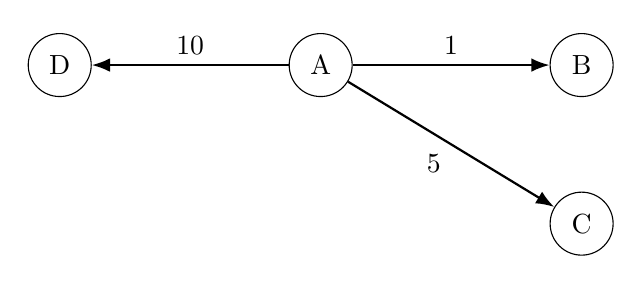
\begin{tikzpicture}[
		node/.style={circle,draw,minimum size=8mm},
		edge/.style={-Latex,thick}
		]
		\node[node] (A) {A};
		\node[node, right=2.5cm of A] (B) {B};
		\node[node, below=1.2cm of B] (C) {C};
		\node[node, left=2.5cm of A] (D) {D};
		
		\draw[edge] (A) -- node[above] {1} (B);
		\draw[edge] (A) -- node[below left] {5} (C);
		\draw[edge] (A) -- node[above] {10} (D);
	\end{tikzpicture}
	\caption{Dopo $A$ vado in $B$. Dopodiché non essendoci altri adiacenti analizzabili torno in $A$ (come se fosse uno stack) e vado al 2° nodo che ha distanza minima da $A$, ovvero $C$}
	\label{fig:grafo-dijkstra}
\end{figure}



\subsection*{5.2.2 Instradamento Distance Vector (DV) / Algoritmo Bellman-Ford}
Se l'instradamento LS usa informazioni globali, quello DV usa solo informazioni locali. DV è distribuito, asincrono e auto-terminante.
\begin{itemize}
	\item Distribuito perché il calcolo viene effettuato su ogni router
	\item Asincrono perché non richiede che tutti i nodi operino al passo con gli altri
	\item Auto-terminante perché non c'è un messaggio chiaro di terminazione: semplicemente quando nota che non c'è più nulla da fare si blocca.
\end{itemize}

Prima di presentare l'algoritmo è bene dapprima presentare la legge di Bellman-Ford.
\\\\
\subsubsection*{Definizioni}
\begin{itemize}
	\item $\delta(x,y)$: costo del percorso minimo da $x$ a $y$
	\item $adj(x)$: insieme dei nodi adiacenti a $x$
	\item $w(x,v)$: peso dell'arco che connette direttamente $x$ e $v$
\end{itemize}

\subsubsection*{Legge}
$$\delta(x,y) = MIN(\forall v \in adj(x), w(x,v) + \delta(v,y))$$

\subsubsection*{Spiegazione della legge}
La formula sta a indicare che il costo minimo da $x$ a $y$ è il minimo $(w(x,v) + \delta(v,y))$ calcolato su tutti i nodi $v$ adiacenti a $x$. Si noti come questa sia una formula ricorsiva in quando $\delta(v,y)$ sarà calcolata allo stesso modo.
\\
\\
La formula di Bellman-Ford fornisce le righe della tabella di inoltro del nodo che la esegue.

\subsubsection*{Algoritmo eseguito dal nodo $x$}
\begin{lstlisting}[escapeinside={(*}{*)}]
BellmanFord()
	
	foreach y in N:
		if y is adjacent:
			(*$\Delta(x,y)$*) = w(x,y)
		else:
			(*$\Delta(x,y)$*) = (*$\infty$*)
	
	foreach v (*$\in$*) adj(x)
		Send(v, (*$\Delta_x$*))
	
	
	wait until either I receive a distance vector 
	from an adjacent or I see a weight changing on 
	the edge connecting me to an adjacent:
		foreach y in N:
			(*$\Delta(x, y)$*) = MIN((*$\forall v \in adj(x), w(x,v) + \Delta(v,y)$*))
		if (*$\Delta_x$*) has changed:
			foreach v (*$\in$*) adj(x)
				Send(v, (*$\Delta_x$*))
\end{lstlisting}

L'algoritmo estende le definizioni con:
\begin{itemize}
	\item $\Delta(x,y)$: \textbf{Stima} della distanza tra $x$ e $y$. Tende a convergere verso $\delta(x,y)$
	\item $\Delta_x$: Vettore che contiene tutti i $\Delta(x,y)$ per ogni $y \in N$ chiamato vettore delle distanze
\end{itemize}

L'algoritmo funziona in questo modo: nella fase di inizializzazione aggiunge al vettore delle distanze i costi verso i suoi vicini e invia a questi ultimi il proprio vettore. Vi è poi una fase di loop perpetuo in cui entra se almeno una delle due condizioni è vera: (1) il costo di un arco verso un proprio vicino cambia oppure (2) riceve il vettore delle distanze da uno dei suoi vicini. Calcola dunque le proprie distanze e se $\Delta_x$ cambia, lo invia ai propri vicini. Questo fa sì che i vicini ottengano una stima più corretta, e, come un effetto domino, tutti i nodi otterranno una stima via via sempre più vicina alla realtà fin quando non si arriva allo stato in cui l'algoritmo si ferma su tutti i nodi, indicando che $\Delta_x = \delta_x \ \forall x \in N$

In alcune situazioni questo algoritmo può portare a instradamenti ciclici.

\subsubsection*{Confronto tra gli istradamenti LS e DV}
Nel DV ciascun nodo dialoga solo con i vicini direttamente connessi, informandoli delle stime da sè stesso a tutti gli altri nodi.

In LS ciascun nodo dialoga con tutti gli altri nodi della rete (nella fase di discovery della topologia della rete), ma comunica loro solo i costi dei collegamenti ad esso direttamente connessi.

Nessuno dei due è Pareto-superior all'altro.

\section*{5.3 Sistemi autonomi e OSPF}
Fino ad ora abbiamo visto i router come unità che eseguono tutti lo stesso algoritmo di instradamento. Questa visione omogenea dei router risulta problematica per i seguenti motivi:
\begin{itemize}
	\item Scalabilità: Al crescere del numero dei router il tempo richiesto per calcolare, memorizzare e comunicare le informazioni di instradamento diventa proibitivo. Inoltre archiviare le informazioni di instradamento su ognuno di essi richiederebbe un'enorme quantità di memoria
	\item Autonomia amministrativa: se si richiedesse che tutti i router del mondo eseguano lo stesso algoritmo di instradamento, significherebbe che gli ISP non avrebbero autonomia amministrativa e libertà di scegliere di utilizzare un algoritmo di instradamento piuttosto che un altro
\end{itemize}

Questi problemi possono essere risolti organizzando i router in sistemi autonomi (AS), composti da gruppi di router sotto lo stesso controllo amministrativo.

Un ISP può scegliere di non utilizzare AS, di unire sotto un unico sistema autonomo tutti i propri router o di partizionare la propria rete in più sistemi autonomi. Ogni sistema autonomo ha un numero identificativo univoco assegnato dallo ICANN (come gli indirizzi IP).

I router di un AS eseguono tutti lo stesso algoritmo di instradamento ma router posti in AS differenti possono usare differenti algoritmi di instradamento.

\subsubsection*{Instradamento intra-AS: OSPF}
In nessun caso è possibile usare direttamente gli algoritmi di Dijkstra e di Bellman-Ford nel mondo reale. Essi sono infatti concettuali in quanto non risolvono problemi pratici come 
\begin{itemize}
	\item Come scopro i vicini?
	\item Che metriche uso?
	\item Come memorizzo le informazioni?
	\item Che protocolli sottostanti uso per comunicare?
	\item Ogni quanto invio informazioni?
	\item Come autentico gli altri router?
	\item ...
\end{itemize}

per questo motivo esistono algoritmi quali OSPF, ISIS, RIP e EIGRP che risolvono questi problemi nella pratica, usando internamente talvolta l'algoritmo LS talvolta DV. Questi algoritmi sono intra-AS, ovverosia funzionano solo all'interno di un sistema autonomo.

Sofferiamoci su OSPF: è un algoritmo di tipo Link-State che utilizza la tecnica del flooding (inondamento di informazioni) affinché tutti i router dell'AS abbiano una mappa della rete aggiornata e completa in modo che l'algoritmo di Dijkstra possa operare efficacemente.

OSPF permette di creare delle partizioni all'interno dell'AS: Ogni sotto-AS (chiamata Area) esegue l'algoritmo Link-State localmente e comunica con altre aree mediante router di confine. Ciò permette più flessibilità e scalabilità in grandi reti, evitando frequenti flooding in tutta l'AS.

\section*{5.4 Instradamento inter-AS: BGP}
Per determinare i percorsi per le coppie sorgente-destinazione che passano per più sistemi autonomi è necessario un algoritmo inter-AS, come BGP. Si tratta di un protocollo di tipo Distance-Vector decentealizzato e asincrono.

\subsection*{5.4.1 Il ruolo di BGP}
BGP determina le tabelle di inoltro esterne all'AS. BGP non instrada però verso uno specifico indirizzo, bensì verso delle sottoreti, come ad esempio \texttt{138.16.68.0/22}. Un sistema autonomo può anche avere più sottoreti ma non è obbligatorio che debbano essere tutte annunciate.

BGP
\begin{itemize}
	\item Consente a ciascuna sottorete di comunicare la propria esistenza al resto di Internet
	\item Determina il percorso migliore verso una sottorete
\end{itemize}

\subsection*{5.4.2 Distribuzione delle informazioni dei cammini in BGP}
Ogni router in ogni sistema autonomo funge o da router gateway, ovvero direttamente connesso a uno o più router di altri sistemi autonomi o da router interno, vale a dire connesso solo a host e altri router interni allo stesso sistema autonomo.

Come viene comunicata l'esistenza di una sottorete verso tutti i sistemi autonomi? In modo molto semplice: una sottorete si annuncia a un AS il quale provvede a comunicarlo a tutti gli AS con cui confina, ripetendo fintantoché tutti i sistemi autonomi non hanno registrato la nuova sottorete. 

Un AS comunica con altri AS tramite i router di bordo: possono esserci anche più router di bordo in uno stesso Sistema Autonomo e possono anche essere non direttamente connessi; in tal caso essi dovranno comunicare mandando messaggi BGP all'interno dell Sistema Autonomo denominati messaggi BGP interni (iBGP). 

I messaggi BGP scambiati tra due router gateway di due AS diversi prendono il nome di messaggi eBGP (external).

\begin{figure}[h]
	\centering
	\includegraphics[width=1\textwidth]{images/eBPG_and_iBGP.png}
	\caption{Connessioni eBGP e iBGP}
	\label{fig:esempio}
\end{figure}

\texttt{1c, 2a, 2c, 3a} e \texttt{3d} sono router di bordo. A titolo di esempio, \texttt{2a} e \texttt{2c} comunicano scambiandosi messaggi BGP interni, mentre \texttt{2c} e \texttt{3a} comunicano scambiandosi messaggi BGP esterni.

\subsection*{5.4.3 Selezione delle rotte migliori}
Quando un router annuncia un prefisso CIDR, aggiunge anche degli attributi BGP:
\begin{itemize}
	\item AS-PATH: Elenca i sistemi autonomi attraverso i quali è passato l'annuncio del prefisso. I router utilizzano tale attributo per evitare annunci ripetuti (se già vedono il loro identificativo al suo interno non lo inoltrano)
	\item NEXT-HOP: Quando un router di bordo di un AS (\textit{x}) riceve un messaggio eBGP da un router di bordo (\textit{y}) di un altro AS  che gli indica l'esistenza di una sottorete, memorizza l'indirizzo IP di \textit{y} come attributo NEXT-HOP che gli permette di sapere a chi inoltrare i pacchetti per raggiungere quel prefisso annunciato. Per un solo prefisso possono esserci più NEXT-HOP. L'indirizzo NEXT-HOP viene poi comunicato a tutti i router interni.
\end{itemize}

\subsubsection*{Instradamento Hot Potato}
Nell'instradamento a patata bollente si cerca di uscire dall'AS il prima possibile, ovverosia si inoltra il pacchetto sul percorso più breve che gli permette di uscire dal Sistema Autonomo. Equivalentemente, si utilizza il percorso verso il NEXT-HOP più vicino che permette di inoltrare il pacchetto alla sottorete desiderata.

Questo algoritmo viene considerato egoista in quanto non garantisce affatto che sia il percorso globalmente migliore per quella destinazione. Se infatti ci si trova molto vicino a un NEXT-HOP, verrà utilizzato quest'ultimo, ma magari il suo AS è molto lontano dalla sottorete di destinazione che sarebbe stata più vicina utilizzando un altro NEXT-HOP iniziale.

\subsection*{5.4.4 Anycast IP}
In molte applicazioni si è interessati a replicare lo stesso contenuto su server differenti sparsi in diverse aree geografiche e che un utente acceda al contenuto dal server che gli è più vicino.

La funzionalità Anycast IP di BGP ci viene in soccorso. Ad esempio una CDN assegna lo stesso indirizzo IP su due o più server fisici differenti i quali annunciano la stessa sottorete al "mondo" BGP. Quando un router BGP riceve annunci da più percorsi li tratta come se fossero percorsi diversi verso la stessa area fisica, anche se sono percorsi verso luoghi diversi.

Il risultato è che gli utenti vengono instradati automaticamente verso l’istanza "più vicina".

Anycast IP è però sconsigliabile in contesti stateful in quanto un cambiamento delle tabelle di routing potrebbe far indirizzare il client a un diverso server fisico durante una sessione di comunicazione, interrompendola. Per questo AnycastIP si usa in contesti stateless, come DNS.

\section*{SDN}
Un'architettura SDN ha queste caratteristiche fondamentali:

\begin{enumerate}
	\item Inoltro basato sui flussi: L'inoltro dei pacchetti può essere fatto da un router sulla base del valore dei campi dell'intestazione a livello di trasporto, di rete o di collegamento
	\item Consente la separazione del piano dati dal piano di controllo: Il piano dei dati consiste di router che eseguono le regole \textit{match-action}. Il piano di controllo consiste di server e software che determinano e gestiscono le tabelle dei flussi dei router. Pertano la rete risulta programmabile da software
\end{enumerate}

\subsection*{5.5.1 Il piano di controllo SDN: controller SDN e applicazioni di controllo}
Il piano di controllo si divide in due componenti: il controller SDN e le applicazioni di controllo SDN.

Le funzionalità del controller SDN possono essere divise in tre livelli:
\begin{enumerate}
	\item Livello di comunicazione: effettua le comunicazioni tra il controller SDN e i dispositivi di rete collegati
	\item Livello di monitoraggio dello stato della rete: Le decisioni di controllo richiedono che il controller abbia informazioni aggiornate circa lo stato di host, collegamenti, router e altri dispositivi
	\item Interfaccia di comunicazione con il livello applicazione di controllo della rete: Le applicazioni sono quelle che leggono/scrivono le tabelle dei flussi
\end{enumerate}

I router inviano informazioni sul loro stato e sui collegamenti a loro connessi al controller SDN, senza scambiare tali informazioni direttamente tra loro. Inoltre, essi non eseguono autonomamente algoritmi di instradamento; è il controller SDN che lo fa. Ciò consente di poter facilmente cambiare l' algoritmo di instradamento semplicemente cambiando il software in un unico punto, anziché doverlo cambiare in ogni router.

\section*{5.6 ICMP}
Il protocollo ICMP (Internet Control Message Protocol) viene utilizzato da host e router per scambiarsi informazioni. È un protocollo a livello di rete.

I messaggi ICMP vengono trasportati come payload di IP, esattamente come segmenti TCP e UDP. Nel datagramma IP è specificato ICMP come protocollo di livello superiore.

I messaggi ICMP contengono:
\begin{itemize}
	\item Un campo "Tipo ICMP" e un campo "Codice" che insieme specificano la tipologia di messaggio ICMP
	\item Se rappresenta un messaggio di errore, contiene anche l'header del datagramma IP che ha provocato l'errore. Non è presente in messaggi informativi (come \textit{ping})
\end{itemize}

Vediamo come funziona traceroute: il programma client invia una serie di datagrammi IP il cui payload è un segmento UDP con un numero di porta improbabile e con un TTL crescente partendo da 1. Quando l'n-esimo router riceve l'n-esimo datagramma, nota che TTL è scaduto, pertanto lo scarta e invia un messaggio di errore ICMP (\textit{TTL expired}).

Ma come fa il programma client a sapere quando fermarsi? Dato che il datagramma contiene un segmento UDP con un numero di porta improbabile, quando giunge a un host (che quindi implementa lo strato di livello di trasporto) quest'ultimo restituisce un errore ICMP di tipo diverso, ovvero \textit{Destination port unreachable}. A questo punto il client smetterà di inviare datagrammi.

\section*{5.8 Riepilogo}
Abbiamo visto che esistono due approcci per la costruzione di un piano di controllo: il controllo tradizionale (nel quale ogni singolo router esegue un algoritmo di instradamento e comunica con gli altri) e il Software-Defined Networking nel quale un controller logicamente centralizzato calcola e gestisce le tabelle di inoltro che devono essere utilizzate dai router.

\chapter{Livello di collegamento e reti locali}
Se il livello di rete fornisce un servizio di comunicazione tra due nodi qualsiasi della rete, il livello di collegamento fornisce un servizio di comunicazione tra due nodi adiacenti.

\section*{6.1 Livello di collegamento: introduzione}
Due nodi adiacenti sono connessi attraverso un collegamento fisico. Per ogni collegamento un nodo trasmittente incapsula il datagramma del livello di rete in un frame del livello di collegamento e lo trasmette al ricevente.

Se il collegamento fisico è condiviso tra più di due nodi ci troviamo dinnanzi un canale broadcast (es. onde elettromagnetiche). D'inverso, se per un dato collegamento ci sono solo due nodi allora siamo in presenza di un canale punto-punto.

\subsection*{6.1.1 Servizi offerti dal livello di collegamento}
Sebbene il servizio base del livello di collegamento sia quello di trasportare datagrammi da un nodo a quello adiacente lungo un singolo canale di comunicazione, i possibili servizi che possono essere forniti dai protocolli a questo livello sono:
\begin{itemize}
	\item Accesso al collegamento: se ci si ritrova in presenza di un canale broadcast è necessario coordinare la trasmissione dei frame (vedere sezione 6.3)
	\item Rilevazione e correzione degli errori: È possibile rilevare e correggere errori nel frame grazie a bit di controllo inseriti nello stesso.
	\item Consegna affidabile: Una conseguenza della rilevazione e correzione degli errori è la consegna affidabile
\end{itemize}

\subsection*{6.1.2 Dov'è implementato il livello di collegamento?}
Per ogni tipologia di collegamento (es. rame, fibra ottica, onde radio) sono stati sviluppati uno o più protocolli di comunicazione. Questi protocolli sono implementati per la maggior parte in hardware, nelle schede di rete (NIC) dei nodi, mentre una parte è implementata in software (come la gestione degli errori e l'incapsulamento dei datagrammi). Il livello di collegamento è dunque dove il software incontra l'hardware.

\section*{6.2 Tecniche di rilevazione e correzione degli errori}
Il nodo trasmittente aggiunge ai dati $D$ che devono essere protetti, dei bit chiamati $EDC$ (Error Detection and Correction).

$D$ e $EDC$, insieme, vengono inviati al ricevente che legge $D'$ e $EDC'$. Esso deve determinare se $D'$ coincida con $D$ avendo solo su $D'$ e $EDC'$.

È importante sottolineare che anche impiegando bit di rilevazione degli errori possono esserci degli errori non rilevati, ovvero si tratta di errori di cui il nodo destinatario non riesce ad accorgersi.

Ci sono tre tecniche per rilevare errori nei dati trasmessi: controllo di parità, checksum e controllo a ridondanza ciclica.

\subsection*{6.2.1 Controllo di parità}
È la forma più semplice di controllo degli errori e utilizza un unico bit di controllo, detto "bit di parità".

Il mittente include un bit addizionale e sceglie il suo valore in modo da rendere pari i bit \texttt{1} nei $d + 1$ bit trasmessi (dove $d$ è il numero di bit in $D$).
\\\\
Esempio:

\begin{Center}
$\underbrace{\mathtt{11011001}}_{D}\;|\underbrace{\mathtt{1}}_{\text{bit di parità}}$
\end{Center}

Ciò che il ricevente deve fare è semplicemente contare il numero di bit \texttt{1} tra quelli ricevuti. Se ne nota un numero dispari allora sa che si è verificato un errore. Questo meccanismo è però molto fragile, infatti se si verifica un numero pari di alterazioni sui bit ci sarà un errore non rilevato. Inoltre può rilevare ma non correggere l'errore.

Vediamo ora un controllo di parià bidimensionale dove i $d$ bit vengono suddivisi in $i$ righe e $j$ colonne. Per ogni riga e per ogni colonna ci sarà un bit di parità, più un ulteriore bit per rilevare errori sugli stessi bit di parità.

Supponiamo ora che si verifichi un errore nei $d$ bit originali: la colonna e la riga dove si è verificato l'errore saranno ora noti e incrociando i dati sarà possibile individuare l'esatto bit corrotto, potendo quindi correggerlo.

\begin{figure}[h]
	\centering
	\includegraphics[width=0.5\textwidth]{images/bdimensional_parity_check.png}
	\label{fig:esempio}
\end{figure}

Anche gli errori sugli stessi bit di parità possono essere individuati e corretti.

\subsection*{6.2.2 Checksum}
Il checksum si basa su questo approccio: i dati sono trattati come interi a 16 bit e sommati. Il complemento a 1 di questa somma costituisce il checksum che viene immesso nell'intestazione.
Il ricevente fa la somma tra i dati ricevuti e il checksum e controlla che il risultato sia 1. Se ci sono degli 0 vuol dire che si è verificato un errore.
(N.D.A. Il libro dice che fa il complemento di questo numero e verifica che il risultato siano tutti 0, ma è un passaggio in più inutile secondo me).

Questo approccio viene però spesso fatto dagli algoritmi di livello di trasporto, mentre il livello di collegamento tende a usare CRC. Perché? Perché il livello di trasporto è implementato in software e quindi ha bisogno di algoritmi semplici e veloci, mentre il livello di collegamento permette di effettuare un controllo sugli errori direttamente nella circuitistica hardware che possono effettuare più rapidamente le complesse operazioni di CRC.

\subsection*{6.2.3 Controllo a ridondanza ciclica (CRC)}
Il controllo a Ridondanza Ciclica è un metodo per rilevare errori ma non per correggerli.

Il messaggio $M$ viene interpretato come un polinomio. Scelto un polinomio $G(x)$ fissato dallo standard di grado $r$, si ottiene $M'$ aggiungendo $r$ zero in coda a $M$.

Si esegue la divisione polinomiale modulo 2 tra $M'(x)$ e $G(x)$, ottenendo un resto $R$.

Il mittente trasmette $T = M|R$ (ovvero concatena $R$ a $M$). Per costruzione, $T$ è divisibile per $G(x)$ con resto $0$.

Il ricevente divide quindi $T(x)$ per $G(x)$ e se vede un resto, vuol dire che si è verificato un errore sui bit.

\textbf{Osservazione:} Quando scriviamo $M$ intendiamo il messaggio (es. \texttt{0110}), quando scriviamo $M(x)$ intendiamo il polinomio ivi associato (es. $x^2+x$). Si tratta dello "stesso oggetto" sotto due punti di vista diversi.

Non dimostreremo la correttezza di CRC.

È un algoritmo molto veloce da fare in hardware.

\section*{6.3 Collegamenti broadcast e protocolli di accesso multiplo}
Il collegamento punto a punto è costituito da un trasmittente posto a un capo del collegamento e da un unico ricevente all'altra

Il collegamento broadcast, invece, può avere più trasmittenti e riceventi e si contendono il collegamento condiviso. Quando un nodo diffonde un frame, tutti gli altri nodi ne ricevono una copia.

Esamineremo ora un problema fondamentale: come coordinare  l'accesso di più nodi trasmittenti e riceventi in un canale broadcast condiviso, ossia analizzeremo il problema dell'accesso multiplo che consiste nel determinare chi e quando debba trasmettere. Il problema viene risolto per mezzo di algoritmi ad accesso multiplo.

Dato che tutti i nodi sono in grado di trasmettere frame, è possibile che due o più lo facciano allo stesso momento, generando una collisione a causa della quale nessuno dei nodi riceventi riuscirà a interpretare i frame. La conseguenza di ciò è anche uno spreco di banda.

Possiamo classificare i protocolli di accesso multiplo in una di queste categorie:
\begin{itemize}
	\item Protocolli a suddivisione del canale
	\item Protocolli ad accesso casuale
	\item Protocolli a rotazione
\end{itemize}

Un protocollo di accesso multiplo per un canale broadcast con banda $R$ bit al secondo dovrebbe idealmente avere le seguenti caratteristiche:
\begin{enumerate}
	\item Quando un solo nodo deve inviare i dati, questo dispone di un throughput pari a $R$ bit al secondo
	\item Quando $N$ nodi devono inviare dati, questi dispongono ciascuno di un throughput pari a $R/N$ bit al secondo
	\item Il protocollo è decentralizzato, in modo che un fallimento di un nodo "master" non causi conseguenze
	\item Il protocollo è semplice in modo che risulti veloce ed economico
\end{enumerate}

\subsection*{6.3.1 Protocolli a suddivisione del canale}
Il multiplexing a divisione di tempo (TDM) e quello a suddivisione di frequenze (FDM) possono essere utilizzati allo scopo.

Nel TDM si assegna ogni slot di tempo a uno degli $N$ nodi in modo tale che ogni nodo abbia un tasso trasmissivo di $R/N$ bit/s.
Il problema di TDM è che anche quando non vi sono altri nodi che devono inviare un pacchetto, quello che vuole trasmettere è vincolato ad attendere il suo turno e quindi trasmetterà a un tasso di $R/N$ sebbene $R$ sia completamente disponibile.

In FDM si suddivide la banda in $N$ frequenze. Anche in questo caso, come in TDM, se non ci sono altri nodi che inviano pacchetti, quello che vuole trasmettere è vincolato a un tasso trasmissivo di $R/N$ bit/s.

Vi è un terzo protocollo a suddivisione del canale denominato accesso multiplo a divisione di codice (CDMA).
CDMA assegna a ogni nodo un codice univoco che inseriscono nei dati inviati. I riceventi, dunque, non devono far altro che leggere solo i segmenti con uno specifico codice.

\subsection*{6.3.2 Protocolli ad accesso casuale}
Qui un nodo trasmette alla massima velocità possibile ma quando si verifica una collisione i nodi riprovano (dopo un certo lasso di tempo casuale non concordato con gli altri nodi) a ritrasmettere ripetutamente i loro frame fin quando non giungono correttamente a destinazione.

Alcuni dei protocolli ad accesso casuale sono ALOHA, CSMA e Ethernet.

\subsubsection*{Slotted ALOHA}
Assumiamo che:
\begin{itemize}
	\item Tutti i frame consistono esattamente di $L$ bit
	\item Il tempo sia suddiviso in slot di $L/R$ secondi (ovverosia esattamente il tempo per trasferire un frame)
	\item I nodi cominciano la trasmissione dei frame solo all'inizio degli slot
	\item I nodi siano sincronizzati in modo che tutti sappiano quando iniziano gli slot
	\item Qualora in uno slot due o più frame collidano, tutti i nodi della rete rilevano l'evento prima del termine dello slot
\end{itemize}

Per collisione intendiamo che uno slot temporale è utilizzato contemporaneamente da almeno due nodi trasmittenti.

Le operazioni dei nodi Slotted ALOHA sono:
\begin{itemize}
	\item Quando un nodo ha un nuovo frame da spedire, attende l'inizio dello slot successivo per trasmetterlo
	\item Se non si verifica una collisione, l'operazione ha avuto successo
	\item Se si verifica una collisione, il nodo la rileva prima del termine dello slot e ritrasmette con probabilità $p$ il suo frame durante gli slot successivi, fin quando l'operazione non ha avuto successo
\end{itemize}

\begin{figure}[H]
	\centering
	\includegraphics[width=0.8\textwidth]{images/slotted_aloha.png}
	\caption{Slotted ALOHA}
\end{figure}

Slotted ALOHA consente a un nodo, qualora fosse il solo nodo attivo della rete, di trasmettere alla massima velocità del canale. Inoltre questo protocollo è anche fortemente decentralizzato anche se è comunque necessario che gli slot siano sincronizzati tra tutti i nodi.

Quando invece ci sono molti nodi attivi, una certa frazione degli slot presenterà collisioni mentre un'altra frazione di essi risulterà vuota a causa della probabilità $(1-p)$ che ogni nodo ha di non trasmettere in quello slot se si è verificata una collisione.

I soli slot non sprecati saranno quelli utilizzati da esattamente un solo nodo per trasmettere. Lo slot in cui si trasmette viene chiamato slot riuscito.

Calcoliamo ora l'efficienza di questo protocollo. Supponiamo che un nodo abbia sempre un frame da spedire e, per semplicità, trasmetta con probabilità $p$ sia un frame che ha colliso sia un nuovo frame. Ipotizziamo di avere $N$ nodi.

La probabilità che un dato slot sia vincente è data dalla probabilità che un solo nodo trasmetta mentre i restanti $N-1$ nodi rimangano inattivi. La probabilità che un solo nodo trasmetta è $p$ mentre la probabilità che $N-1$ nodi non trasmettano è $(1-p)^{N-1}$. Quindi la probabilità di successo di un dato nodo è $p(1-p)^{N-1}$.
Poiché ci sono $N$ nodi, la probabilità che un nodo arbitrario abbia successo è $Np(1-p)^{N-1}$.

Il valore $p*$ che sostituito a $p$ massimizza l'espressione è $0,37$. Pertanto, impostiamo questo valore come valore di $p$. Ne consegue che i nodi trasmetteranno informazione utile non più del $37\%$ delle volte e quindi la banda effettivamente utilizzata sarà al più del $37\%$

\subsubsection*{ALOHA}
Slotted ALOHA richiede che tutti i nodi sincronizzino le loro trasmissioni mentre ALOHA è completamente decentralizzato.

Supponiamo che tutti i frame abbiano stessa dimensione e supponiamo che la trasmissione di un frame inizi a $t_0$. Ciò implica che nessun altro nodo può cominciare la trasmissione di un frame nell'intervallo $(t_0-1 , t_0]$ né può iniziare nell'intervallo $[t_0, t_0+1]$ altrimenti i due frame si sovrapporrebbero (vedi figura)

\begin{figure}[H]
	\centering
	\includegraphics[width=0.8\textwidth]{images/aloha_interference.png}
\end{figure}

ALOHA ha un'efficienza peggiore di Slotted ALOHA, ma è il prezzo per essere completamente decentralizzato.

\subsubsection*{CSMA: Accesso multiplo con rilevamento della portante}
Nei due protocolli ALOHA i nodi prendono la decisione di parlare indipendentemente dall'attività degli altri nodi.

CSMA invece si basa sul seguente principio: Ascoltare prima di parlare. Un nodo ascolta il canale prima di trasmettere. Se un canale sta già trasmettendo un frame, il nodo aspetta. Questa caratteristica si chiama rilevamento della portante.

Nonostante ciò possono comunque verificarsi collisioni. Perché? Per capirlo si guardi il seguente grafico dove l'asse delle $x$ rappresenta lo spazio e le lettere suindicate rappresentano dei nodi. A titolo di esempio, la distanza tra $A$ e $C$ è maggiore della distanza tra $A$ e $B$. L'asse delle $y$ rappresenta il tempo. 


\begin{figure}[h]
	\centering
	\includegraphics[width=0.5\textwidth]{images/CSMA_space_time_diagram.png}
	\caption{Diagramma spazio-temporale di CSMA con collisioni}
\end{figure}

Sia il nodo B che il nodo D vogliono mandare un segmento. B lo fa a tempo $t_0$ ma poiché il tempo di propagazione del segmento da B a D è non nullo, a tempo $t_1$ il nodo D vede il canale libero (anche se non lo è) e immette nella rete i suoi segmenti, generando una collisione.

Il ritardo di propagazione da un estremo all'altro della rete è cruciale: maggiore sarà questo ritardo maggiori saranno le possibilità di collisione.

\subsubsection*{CSMA/CD: Accesso multiplo con rilevazione della portante e delle collisioni}
CSMA/CD estende CSMA in questo modo: Il nodo che trasmette rimane in ascolto del canale. Se osserva che un altro nodo sta trasmettendo un frame che interferisce col suo, cessa immediatamente la propria trasmissione.

La differenza con CSMA è che quest'ultimo non rimane in ascolto mentre invia il frame.

Grazie a CSMA/CD la durata della collisione diminuisce

\subsection*{6.3.3 Protocolli a rotazione}
Esistono diversi protocolli a rotazione ma qui ne citiamo due:

\subsubsection*{Protocollo polling}
Uno dei nodi, designato come principale, interpella a turno gli altri. Il nodo principale invia un messaggio al nodo 1 indicandogli che può trasmettere per un determinato periodo di tempo, dopodiché passa al nodo 2 e così via. Se un nodo non deve comunicare o la sua trasmissione dura meno della finestra temporale a lui assegnata, il nodo principale passa immediatamente al successivo.

Il protocollo polling elimina le collisioni e gli slot vuoti ma introduce degli svantaggi: il primo è l'introduzione del ritardo di polling, il secondo è che se il nodo principale si guasta, la rete collassa.

\subsubsection*{Protocollo token-passing}
Qui non esiste un nodo principale ma c'è un messaggio di controllo, detto token, che passa da un nodo all'altro in ordine prefissato. Solo chi ha il token è autorizzato a comunicare. Questo protocollo è completamente decentralizzato ma se un nodo si guasta o se non riesce a inoltrare il token la rete collassa.

\section*{6.4 Reti locali commutate}
Gli switch operano a livello di collegamento e commutano frame. Non riconoscono gli indirizzi a livello di rete. Affinché sia possibile commutare frame, si utilizzano indirizzi a livello di collegamento.

\subsection*{6.4.1 Indirizzi a livello di collegamento e ARP}
Host e router hanno indirizzi a livello di collegamento, detti indirizzi MAC. Inoltre analizzeremo il protocollo ARP che fornisce ai nodi un meccanismo per trasformare indirizzi IP in indirizzi MAC

\subsubsection*{Indirizzi MAC}
Gli indirizzi MAC sono composti da 6 byte, solitamente scritti in modo esadecimale. Esempio: \texttt{49-BD-D2-C7-56-2A}. Gli indirizzi MAC sono "piatti" ovvero non hanno una struttura gerarchica.

Così come gli indirizzi IP, non sono i nodi in sè ad avere un indirizzo MAC, bensì sono le loro interfacce di rete a possederli. Non esistono al mondo due NIC con lo stesso indirizzo MAC. È la IEEE che assegna a ogni casa madre un blocco. 

È importante sottolineare che gli switch NON hanno indirizzi di collegamento associati alle loro interfacce in quanto il loro compito è trasportare frame in modo trasparente. Questo significa che i nodi non devono esplicitamente inserire l'indirizzo MAC dello switch che interviene.

Quando una scheda di rete vuole inviare un frame, inserisce in quest'ultimo l'indirizzo MAC del destinatario e lo immette nella rete. Uno switch può occasionalmente fare broadcast di un frame in ingresso su tutte le sue interfacce di uscita, pertanto una scheda di rete può ricevere un frame non indirizzato a lei. In tal caso la scheda di rete scarterà il frame.

Se viene inserito l'indirizzo di broadcast \texttt{FF-FF-FF-FF-FF-FF}, tutte le schede di rete nella sottorete otterranno il frame.

\subsubsection*{Protocollo per la risoluzione degli indirizzi: ARP}
Dato che esistono sia indirizzi del livello di rete sia indirizzi a livello di collegamento, si ha la necessità di tradurre l'indirizzo IP in indirizzo MAC.

Un modulo ARP è presente su tutti i nodi (non sugli switch): riceve un indirizzo IP e determina l’indirizzo MAC associato. ARP risolve soltanto gli indirizzi IP per i nodi della stessa sottorete. È in grado di fare ciò per mezzo di una tabella ARP che contiene la corrispondenza degli indirizzi più un valore relativo al TTL che indica quando bisogna eliminare una voce dalla tabella.


\begin{table}[h!]
	\centering
	\begin{tabular}{|c|c|c|c|}
		\hline
		\textbf{Indirizzo IP} & \textbf{Indirizzo MAC} & \textbf{TTL}\\
		\hline
		10.0.0.2 & A2:A3:42:B5:58:84 & 12:48 \\
		10.0.0.3 & 7A:0F:44:27:5D:5A & 13:53 \\
		\hline
	\end{tabular}
	\caption*{Esempio di tabella ARP in un modulo ARP}
\end{table}

La tabella non contiene necessariamente una voce per ogni nodo. Ma allora che cosa succede quando arriva un indirizzo IP di cui non si conosce l'indirizzo MAC? In questo caso il nodo costruisce un pacchetto ARP, contenente l'indirizzo IP da risolvere e lo invia all'indirizzo broadcast \texttt{FF-FF-FF-FF-FF-FF}. Il suo scopo è interrogare tutti gli altri nodi della sottorete riguardo l'indirizzo MAC corrispondente all'indirizzo IP da risolvere.

Il frame contenente la richiesta ARP è ricevuto da tutte le schede di rete della sottorete che controllano se il proprio indirizzo IP coincide con quello richiesto. In caso affermativo viene inviata una risposta ARP con l'indirizzo MAC associato. Questo frame non viene inviato in un frame broadcast.

ARP è un protocollo a livello di collegamento o a livello di rete? Un pacchetto ARP è incapsulato in un frame a livello di collegamento, quindi giacerebbe sopra di esso. D'altro canto contiene anche indirizzi a livello di collegamento, pertanto apparterrebbe ad esso. Contiene inoltre indirizzi a livello di rete e quindi, in teoria, apparterrebbe anche a quest'ultimo. Alla fine possiamo considerare ARP essere un protocollo al confine tra il livello di rete e quello di collegamento.

\subsubsection*{Come inviare un datagramma a un nodo esterno alla sottorete}
Ipotizziamo che un datagramma dalla sottorete A deve viaggiare verso la sottorete B. Ipotizziamo che tra A e B ci sia esattamente un router. Quest'ultimo presenta due interfacce: una esposta verso A e una verso B.

Al datagramma viene assegnato l'indirizzo IP di destinazione dell'host nella rete B, ma quando viene incapsulato in un frame, quest'ultimo non avrà l'indirizzo MAC dell'host di destinazione, bensì avrà l'indirizzo MAC della porta del router rivolta verso A.

Il router, quando invia il frame dalla propria interfaccia rivolta verso B, inserirà l'indirizzo MAC dell'host di destinazione.

\subsection*{6.4.2 Ethernet}
Negli anni '70 Ethernet usava un cavo coassiale con topologia a bus. Questa topologia era un canale broadcast.

Alla fine degli anni '90 si era evoluta utilizzando un cavo di rame con una topologia a stella basata su hub. Un hub è un dispositivo di rete che quando riceve un bit da una delle sue interfacce, lo inoltra identico verso tutte le altre interfacce. Anche in questo caso siamo dinnanzi un canale broadcast.

All'inizio degli anni 2000 lo switch prende il posto dell'hub. Uno switch è un commutatore di pacchetti di livello di collegamento e garantisce che non ci siano collisioni grazie all'impiego di buffer.

\subsubsection*{Struttura dei frame Ethernet}
Esaminiamo i campi di un frame Ethernet:
\begin{itemize}
	\item Campo dati (da 46 a 1500 byte): Contiene il datagramma IP. Dato che l'unità massima di trasmissione (MTU) è 1500 byte, se il datagramma IP supera questo valore allora deve essere frammentato. Se invece è inferiore a 46byte deve allora essere riempito fino a raggiungere questo valore
	\item Indirizzo MAC destinazione
	\item Indirizzo MAC sorgente
	\item Tipo: Indica il protocollo superiore a cui deve essere consegnato il payload nel nodo destinatario. Questo perché IP non è l'unico protocollo superiore che esiste. Infatti troviamo ad esempio ARP.
	\item CRC
	\item Preambolo: I frame Ethernet iniziano con 7 byte tutti uguali che servono risvegliare le schede di rete e sincronizzare il loro clock mentre un altro byte, differente, indica che i dati veri e propri stanno per arrivare 
\end{itemize}

Ethernet fornisce un servizio non orientato alla connessione: i frame vengono immessi nella rete senza alcun handshake. Inoltre fornisce un servizio non affidabile, infatti, anche se il controllo CRC fallisce, non lo segnala al mittente; semplicemente lo scarta. Ciò aiuta a mantenere Ethernet semplice ed economico.

Quando Ethernet era basato su bus o a centro-stella con hub, si trattava di un canale broadcast. Pertanto veniva impiegato il protocollo CSMA/CD. Oggi, dato che ci troviamo in contesti a centro-stella con switch, non ci sono collisioni e pertanto non vi è la necessità di operare un protocolli ad accesso multiplo.

\subsection*{6.4.3 Switch}
Il ruolo dello switch è quello di ricevere frame in ingresso e inoltrarli sui collegamenti in uscita. Lo switch è "trasparente" ai nodi in quanto questi ultimi si indirizzano frame l'un l'altro senza indirizzarli direttamente allo switch. In altre parole, dal punto di vista dei nodi, lo switch non esiste. Le interfacce degli switch hanno dei buffer

\subsubsection*{Inoltro e filtraggio}
Il filtraggio è la funzionalità dello switch che determina se un frame debba essere inoltrato a una qualche interfaccia o scartato. L'inoltro consiste nell'individuazione dell'interfaccia su cui il frame debba essere diretto e dell'invio su di essa.

Le operazioni di inoltro e filtraggio su uno switch sono eseguite mediante una tabella di commutazione composta da una riga per ogni nodo, sebbene non sia necessario che tutti i nodi siano presenti nella tabella di commutazione. Le righe contengono: (1) Indirizzo MAC del nodo, (2) l'interfaccia dello switch che conduce al nodo, (3) il momento in cui quella voce è stata creata.

Ipotizziamo che un frame con indirizzo di destinazione \texttt{AA-AA-AA-AA-AA-AA} giunga allo switch sull'interfaccia $x$. Lo switch cerca nella sua tabella di commutazione l'indirizzo MAC \texttt{AA-AA-AA-AA-AA-AA}. I possibili casi sono 3:
\begin{enumerate}
	\item Non vi è una voce per l'indirizzo \texttt{AA-AA-AA-AA-AA-AA}. In questo caso lo switch inoltra il frame a tutte le interfacce tranne $x$.
	\item Vi è una voce che associa \texttt{AA-AA-AA-AA-AA-AA} all'interfaccia $x$. In questo caso la destinazione proviene dal segmento di rete da cui ha ricevuto il frame, pertanto lo scarta
	\item Una voce della tabella associa \texttt{AA-AA-AA-AA-AA-AA} a un'interfaccia $y$ con $y \neq x $. In questo caso il frame viene inoltrato su $y$.
\end{enumerate}

\subsubsection*{Autoapprendimento}
Gli switch hanno la proprietà di costruire automaticamente e dinamicamente le proprie tabelle, senza l'ausilio di un operatore o di un protocollo. Questa capacità è ottenuta nel seguente modo:

\begin{enumerate}
	\item La tabella è inizialmente vuota
	\item Di ogni frame che riceve, lo switch archivia nella sua tabella l'indirizzo MAC del campo sorgente del frame, l'interfaccia da cui è arrivato e il momento di arrivo. In tal modo registra il segmento di rete su cui risiese il nodo trasmittente. Quando tutti i nodi della sottorete avranno inviato un frame, allora la tabella sarà completa.
	\item Dopo un certo periodo di tempo in cui lo switch non riceve un frame da un determinato indirizzo sorgente, lo elimina dalla tabella	
\end{enumerate}

Gli switch sono dunque dispositivi plug-and-play

\subsubsection*{Proprietà della commutazione a livello di collegamento}
Possiamo identificare svariati vantaggi utilizzando gli switch al posto dei collegamenti broadcast come i bus o gli hub:
\begin{enumerate}
	\item Eliminazione delle collisioni: non vi è spreco di banda a causa delle collisioni. Gli switch mettono i frame nei propri buffer e non trasmettono più di un frame per ogni segmento in un certo istante
	\item Collegamenti eterogenei: Grazie agli switch i vari collegamenti possono funzionare a velocità diverse e usare cavi diversi
	\item Gestione: Se una scheda di rete ha un malfunzionamento, lo switch lo rileva e la disconnette dalla rete
\end{enumerate}

\subsubsection*{Switch e router a confronto}
Sia i router che gli switch sono commutatori store-and-forward. Il primo è a livello di rete mentre il secondo è a livello collegamento.

La topologia di una rete switch deve necessariamente essere ad albero per evitare cicli di frame broadcast. Inoltre se la rete è troppo grande richiede enormi tabelle ARP.

Nei router i datagrammi rischiano di percorrere cicli solo se le tabelle di routing sono configurate male. Anche in quel caso, però, il danno sarebbe limitato grazie al TTL. Pertanto qui non siamo limitati a una topologia ad albero. I router, però, non sono plug-and-play e a causa del fatto che devono elaborare protocolli a un livello più sopra sono generalmente più lenti.

\subsection*{6.4.4 LAN virtuali}
Immaginiamo una LAN universitaria suddivisa in dipartimenti grazie a degli switch. Con questo approccio ci sono delle problematiche:
\begin{itemize}
	\item Mancanza di isolamento del traffico: Il traffico broadcast come quello ARP, DHCP o messaggi la cui destinazione è ancora sconosciuta per gli switch attraversano l'intera rete accademica.
	\item Uso inefficiente degli switch: Per ogni nuovo dipartimento è necessario comprare un nuovo switch.
	\item Gestione inefficiente degli utenti: Se un utente si muove tra più dipartimenti, deve collegarsi di volta in volta a switch differenti.
\end{itemize}

Queste difficoltà possono essere superate grazie alle LAN Virtuali (VLAN).

Gli host all'interno di una VLAN comunicano come se fossero i tutti e i soli connessi allo switch. Inoltre, una VLAN è un dominio broadcast, il che significa che i messaggi broadcast non vengono replicati sulle altre VLAN.

In una VLAN le interfacce di uno switch vengono suddivise in gruppi, ognuno dei quali costituisce una VLAN.

Isolando le VLAN, come trasmettiamo il traffico da un dipartimento a un altro? Lo facciamo per mezzo di un router (che può essere anche integrato nello stesso apparato di rete). I due dipartimenti apparirebbero come se ognuno avesse degli switch separati interconnessi da un router.

Adesso immaginiamo di avere più switch: l'originale A suddiviso in VLAN Ingegneria e VLAN Filosofia e lo switch B appena comprato. Vogliamo fare in modo che B possa egualmente essere suddiviso in VLAN Ingegneria e VLAN Filosofia e che le VLAN dello stesso tipo, seppure su switch diversi, possano parlarsi.

Una soluzione è connettere un cavo da una porta VLAN Ingegneria di A a una porta dello switch B e fare lo stesso con la VLAN di Filosofia. Dopodiché suddividere lo switch B in 2 VLAN. (Figura 6.26a). Abbiamo sprecato 2 porte sullo switch A e 2 porte sullo switch B. Non è una soluzione scalabile.

Un altro approccio è chiamato VLAN Trunking: una porta speciale, detta porta di trunking, viene configurata sui due switch. La porta di trunking appartiene a tutte le VLAN. I frame inoltrati a una qualunque VLAN vengono inoltrati anche sulla porta di trunking. Questo fa sì che il risultato è come se fosse un unico grande switch.

Ci siamo concentrati sulle VLAN basate sulle porte, ma esistono anche VLAN basate su indirizzi MAC (un insieme di indirizzi MAC fa parte di una VLAN, un altro insieme fa parte di un'altra VLAN).

\section*{6.5 Canali virtuali: una rete come un livello di collegamento}
Abbiamo iniziato il capitolo considerando il collegamento come un cavo fisico che collega due host. In realtà, il collegamento potrebbe essere una complessa struttura commutata. Gli host continuano a vederlo come se fosse un singolo cavo.


\chapter{Network Security}
Siano Alice e Bob due entità che vogliono comunicare in modo sicuro. Cosa vuol dire ciò?

Innaizututto si vuole che solo i veri destinatari possano leggere un messaggio inviato, anche se la comunicazione avviene su un canale insicuro. Alice e Bob vogliono inoltre assicurarsi che le persone con cui stanno comunicando siano effettivamente chi dicono di essere e vogliono che i loro messaggi non vengano alterati in transito.

Dati questi presupposti, identifichiamo le seguenti proprietà desiderabili di una comunicazione sicura:
\begin{itemize}
	\item Confidenzialità: Solo Alice e Bob dovrebbero poter leggere il contenuto del messaggio
	\item Integrità: Alice e Bob vogliono che il contenuto della loro comunicazione non venga alterato in transito
	\item Autenticazione: I comunicanti devono poter confermare l'identità del loro corrispondente per accertarsi che siano effettivamente chi dicono di essere
	\item Operational Security: Firewall e sistemi anti-intrusione dovrebbero essere usati per rilevare e fermare attacchi
\end{itemize}

Senza queste caratteristiche, infatti, un malfattore potrebbe:
\begin{itemize}
	\item Intercettare e memorizzare i mesaggi sul canale
	\item Modificare o eliminare i messaggi o inserirne di nuovi
\end{itemize}
che gli consentirebbe di impersonare un'altra entità, rubare informazioni, negare l'acesso alla rete a utenti legittimi ecc...

La crittografia tornerà utile non solo per fornire confidenzialità, ma anche integrità e autenticazione.

\section*{8.2 Principi di crittografia}
Un messaggio nella sua forma originale è detto plaintext. Una volta criptato per mezzo di un algoritmo di crittografia assumerà il nome di messaggio cifrato che risulta illeggibile agli occhi di un intrusore.

Sommariamente funziona così: se Alice vuole invire un messaggio a Bob, dà $m$, il plaintext, in pasto a un algoritmo di crittografia insieme a una chiave che chiamaremo $K_A$. Denotiamo con $K_A(m)$ il messaggio cifrato. Bob darà in pasto a un algoritmo di decrittografia il messaggio cifrato che ha ricevuto e la sua chiave, $K_B$. Il messaggio così ottenuto sarà il messaggio nella sua forma originale, ovvero $K_B(K_A(m)) = m$.

In un sistema a chiave simmetrica le due chiavi saranno identiche ($K_A = K_B$) e conosciute solo ad Alice e Bob. In un sistema a chiave pubblica si utilizza una coppia di chiavi per ogni interlocutore. Una delle due chiavi è pubblica e fatta conoscere a tutti, mentre l'altra è segreta (solo l'interlocutore che l'ha generata la conosce).

\subsection*{8.2.1 Crittografia a chiave simmetrica}
Nella crittografia a chiave simmetrica i due interlocutori hanno la stessa chiave ma il problema di questo approccio è che hanno bisogno di un canale sicuro per scambiarsela. Di certo non possono inviarla su un sistema insicuro altrimenti un malfattore potrebbe intercettarla e rendere vana la crittografia

\subsubsection*{Block ciphers}
In una crittografia a block cipher, un messaggio viene suddiviso in blocchi da $k$ bit. Ogni blocco viene crittografato indipendentemente per mezzo di una tabella di corrispondenza che fa corrispondere ogni possibile valore del blocco in un altro valore. Ad esempio se $k=3$ avremo una tabella grande $8$ righe che farà corrispondere, ad esempio, il valore $110$ in $010$. Queste modalità di cifratura presenta problematiche: se $k$ è troppo piccolo allora viene facilmente bucato; se $k$ è troppo grande, i nodi devono memorizzare una tabella enorme.

Una metodologia oggi utilizzata invece consiste nel suddividere il messaggio in blocchi grandi (ad esempio) $64$ bit. Ogni blocco viene ulteriormente suddiviso in $8$ chunk grandi $8$ bit. Per ogni chunk ci sarà una tabella di corrispondenza grande $2^8$ bit (e quindi ci saranno $8$ tabelle grandi $2^8$, che è molto inferiore a $2^64$). Dopodiché gli $8$ chunk da $8$ bit vengono riassemblati in un unico blocco da $64$ bit. Per aumentare la sicurezza, un permutatore modifica il valore di questi $64$ bit e ripete il ciclo $n$ volte, dando come input all'$n$esimo ciclo il valore di output ottenuto nel $(n-1)$esimo ciclo.

La chiave di decodifica di questo algoritmo sono le 8 tabelle di corrispondenza.

Algoritmi di questo genere sono il DES e l'AES.

\subsection*{8.2.2 Public Key Encryption}
Per superare le difficoltà della crittografia a chiave simmetrica si è sviluppata la crittografia a chiave pubblica.

Invece di far condividere a Bob e Alice la stessa chiave, affinché Alice possa mandare un messaggio sicuro a Bob, adesso quest'ultimo ha due chiavi: una pubblica, visualizzabile da chiunque e una privata, conosciuta solo a Bob. La notazione $K^{+}_{B}$ si riferice alla chiave pubblica di Bob mentre $K^{-}_{B}$ si riferisce a quella privata.

Alice cifra il messaggio $m$ con la chiave pubblica di Bob, ovvero calcola $K^{+}_{B}(m)$ e gli invia il risultato. Dall'altro capo della comunicazione, Bob usa la sua chiave privata per decifrare il messaggio inviato da Alice, calcolando $K^{-}_{B}(K^{+}_{B}(m))$. In questo modo Alice può inviare un messaggio leggibile solo da Bob senza doversi scambiare alcuna chiave condivisa!

Avremo inoltre che $K^{-}_{B}(K^{+}_{B}(m))$ = $K^{+}_{B}(K^{-}_{B}(m))$ = $m$

Un messaggio cifrato con una chiave può essere decifrato solo e soltanto con l'altra chiave.

La crittografia a chiave pubblica introduce uno svantaggio: poiché la chiave di cifratura è pubblica, chiunque può inviare un messaggio a Bob, incluso qualcuno che si finge essere Alice. Pertanto Bob non ha modo di conoscere se il mittente è davvero chi dice di essere. Nella crittografia a chiave simmetrica questo non avviene perché solo il fatto che il messaggio è stato cifrato con una chiave segreta conosciuta solo ai due implicitamente garantisce che il corrispondente è davvero chi dice di essere.

\section*{8.3 Integrity and Authentication}
Affinché Bob possa fidarsi del messaggio ricevuto deve verificare
\begin{enumerate}
	\item Che il messaggio sia stato originato davvero da Alice (Authentication)
	\item Il messaggio non è stato modificato in transito (Integrity)
\end{enumerate}

\subsection*{8.3.1 Cryptographic Hash Functions}
Una funzione hash prende in input $m$ e calcola una stringa di lunghezza fissa $H(m)$. Inoltre, deve essere studiata affinché sia computazionalmente difficile trovare un $n$ tale che $n \neq m$ ma $H(m) = H(n)$.

Gli algoritmo MD5 e SHA sono le funzioni di hash crittografico più utilizzate.
\subsection*{8.3.2 Message Authentication Code (MAC)}
Vediamo come potremmo implementare un meccanismo di integrità dei messaggi:
\begin{enumerate}
	\item Alice crea un messaggio $m$ e calcola l'hash $H(m)$
	\item Alice concatena $H(m)$ al messaggio ottenendo $(m, H(m))$
	\item Bob riceve $(m,h)$ e calcola $H(m)$. Se $H(m) = h$ allora conclude che va tutto bene 
\end{enumerate}

Questo ragionamento è piuttosto fallace, infatti, un fuorilegge potrebbe creare un messaggio $m'$, calcolare $H(m')$ e mandare a Bob $(m', H(m'))$ dicendo di essere Alice. Dunque, per implementare correttamente la funzionalità di integrità dei messaggi, Alice e Bob dovrebbero scambiarsi una chiave segreta $s$ denominata chiave di autenticazione. Vediamo come funziona:
\begin{enumerate}
	\item Alice crea il messaggio $m$, concatena $s$ a $m$ e calcola la funzione hash $H(m+s)$. $H(m+s)$ viene definito Message Authentication Code (MAC)
	\item Alice invia a Bob il messaggio $m$ e il MAC, ovvero invia $(m, H(m+s))$
	\item Bob riceve $(m,h)$ e calcola $H(m+s)$. Se quest'ultimo coincide con $h$ allora conclude che va tutto bene.
\end{enumerate}

Si noti come non vi è la necessità di adoperare un algoritmo di cifratura se le parti si preoccupino solo dell'integrità ma non della confidenzialità.

Come distribuire la chiave $s$? Semplicemente si può mandare a un nodo cifrandola con la sua chiave pubblica.

\subsection*{8.3.3 Firma digitale}
Si vuole che sia possibile provare che un documento sia stato firmato da un individuo (verificabilità) e che solo quell'individuo possa averlo fatto (la firma non può essere falsificata).

Si supponga che Bob voglia firmare un documento $m$. Semplicemente usa la sua chiave privata per calcolare $K^{-}_{B}(m)$ in odo che chiunque possa usare $K^{+}_{B}$ per ottenere il documento. Qui l'obiettivo di B non è quello di offuscare il contenuto ma è quello di firmarlo in modo verificabile e infalsificabile.

Alice riceve $(m, K^{-}_{B}(m))$. Per verificare che sia stato Bob a firmare il documento, utilizza la chiave pubblica di B per ottenere $m$. Ovvero fa $K^{+}_{B}(K^{-}_{B}(m))$. Dato che solo Bob può aver utilizzato $K^{-}_{B}$, conclude che sia stato lui a firmarlo.

Si noti che se il messaggio fosse modificato in un modo da ottenere $m'$, si otterrebbe $m' \neq K^{+}_{B}(K^{-}_{B}(m))$ concludendo che la firma non è valida.

In realtà nel mondo reale non si fa davvero così: anziché fare $K^{-}_{B}(m))$ per poi fare $K^{+}_{B}(K^{-}_{B}(m))$ si fa $K^{-}_{B}(H(m)))$ per poi fare $K^{+}_{B}(K^{-}_{B}(H(m)))$, ovverosia si agisce sul risultato della funzione hash dato che è generalmente più piccola di un intero messaggio.

\subsubsection*{Public Key Certification}
Come certificare che una chiave pubblica appartenga a un'entità specifica? Un'Autorità di Certificazione (CA) si assicura che un'entità è effettivamente chi dice di essere. Una volta assicurato ciò, la CA crea un certificato che associa la chiave pubblica all'entità (identificata per mezzo di un identificatore univoco, come l'indirizzo IP). Il certificato è firmato digitalmente dalla CA.

\section*{8.4 Endpoint Authentication}
Nella sezione 8.3 abbiamo visto come Bob possa verificare che l'autore di un messaggio ricevuto in qualunque momento passato sia effettivamente Alice. 

Ora vediamo un altro aspetto: come autenticare la controparte in un contesto "in diretta". Lo si fa per mezzo di un protocollo di autenticazione (AP).

\subsubsection*{AP 1}
L'algoritmo AP1 consiste che Alice dica a Bob di essere Alice. Questo algoritmo è debole in quanto il malintenzionato può semplicemente dire a Bob di essere Alice, anche se non lo è.

\subsubsection*{AP 2}
L'algoritmo AP2 consiste che Alice dica a Bob di essere Alice. Bob conosce l'indirizzo reale di Alice e lo confronta con l'indirizzo sorgente del messaggio appena ricevuto. Se coincide considera la controparte autenticata. Anche questo protocollo è debole: un malintenzionato potrebbe creare un pacchetto malevole contenente come indirizzo sorgente l'indirizzo reale di Alice. Questa tecnica si chiama IP Spoofing.

\subsubsection*{AP 3}
AP3 introduce il concetto di password. Alice deve autenticarsi con una password ma il malintenzionato potrebbe semplicemente mettersi in ascolto sulla comunicazione (sniffing) e rilevare la password.

\subsubsection*{AP 3.1}
Adesso ipotizziamo che la password venga cifrata con una chiave simmetrica. Adesso il malintenzionato non conosce più la password in plaintext, ma cambia poco in quanto egli può effettuare il cosiddetto attacco playback. Si tartta di memorizzare la password cifrata che ha ottenuto mettendosi in ascolto sul canale, memorizzare la password cifrata e presentarla a Bob in un secondo momento. Quest'ultimo penserà incorrettamente che si tratti di Alice.

\subsubsection*{AP 4}
Introduciamo il concetto di nonce: si tratta di un numero che il protocollo userà solo una volta durante tutta la sua vita.

AP 4 funziona in questo modo:
\begin{enumerate}
	\item Alice si annuncia a Bob dicendo di essere Alice
	\item Bob sceglie un nonce, $R$, e lo invia ad Alice
	\item Alice critta $R$ usando la chiave simmetrica conosciuta tra i due e invia $K(R)$ a Bob.
	\item Bob decifra il messaggio e se coincide con $R$ allora si assicura che sta parlando con la "vera" Alice. Il fatto che Alice conosca $K$ la autentica
\end{enumerate}

Se un malintenzionato registra il pacchetto contenente $K(R)$ e lo reinvia a Bob, questi lo scarterà in quanto risulta già utilizzato.

\section*{8.5 Securing E-mail}
È possibile offrire servizi di sicurezza a qualunque dei 4 livelli più in alto dello stack. Adesso concentriamoci sul livello applicazione, in particolare sull'email. Uno degli algoritmi più utilizzati in questo contesto è Pretty Good Privacy (PGP).

Supponiamo che Alice e Bob si preoccupino solo della confidenzialità ma non dell'integrità e autenticazione. In questo caso Bob rende la sua chiave pubblica accessibile a chiunque. Alice critta il messaggio verso Bob con la chiave pubblica di Bob, dopodiché glielo invia. Quando Bob riceve il messaggio, lo decritta con la sua chiave privata.
In realtà cifrare e decifrare lunghi messaggi con le chiavi pubbliche e private è oneroso. Per tale motivo ciò che realmente accade è:
\begin{enumerate}
	\item Alice sceglie una chiave simmetrica $K_s$
	\item Cifra il messaggio $m$ con $K_s$
	\item Cifra la chiave simmetrica $K_s$ con la chiave pubblica di Bob
	\item Crea un messaggio $(K_s(m), K^{+}_{B}(K_s))$ e lo invia a Bob (ovvero manda il messaggio cifrato con la chiave simmetrica e manda la chiave simmetrica cifrata con la chiave pubblica di Bob)
	\item Bob decifra la chiave simmetrica (che è molto più semplice che decifrare $m$) e grazie ad essa decifra il messaggio
\end{enumerate}

Adesso supponiamo che Alice e Bob non si preoccupino della confidenzialità ma solo dell'autenticazione e integrità dei messaggi (il contenuto del messaggio è dunque visibile a chiunque). Allora avviene quanto segue:
\begin{enumerate}
	\item Alice crea il digest del messaggio con $H(m)$
	\item Cifra $H(m)$ con la propria chiave pubblica: $ K^{-}_{A}(H(m))$
	\item Crea un messaggio $(m, K^{-}_{A}(H(m)))$ e lo invia a Bob
	\item Quando Bob riceve il messaggio, calcola $H(m)$ e lo confronta con $K^{+}_{B}(K^{-}_{A}(H(m)))$. Se coincide, allora ha autenticato Alice.
\end{enumerate}

Adesso pogettiamo un algoritmo che offra confidenzialità, autenticazione e integrità: Alice compie gli stessi passi descritti poc'anzi per quando vuole offrire semplice autenticazione e integrità, ma anziché inviare $(m, K^{-}_{A}(H(m)))$, lo tratta come un semplice messaggio di cui assicurare confidenzialità, pertanto lo cifra con la chiave privata di Bob (in realtà, come abbiamo visto, lo cifra con $K_s$ per poi cifrare $K_s$ con la chiave privata di Bob). Alice quindi usa la crittografia a chiave pubblica/privata due volte: una volta con la propria chiave privata e una volta con la chiave pubblica di Bob. Anche Bob, similmente, la userà due volte.

Perché facciamo questo? Lo facciamo perché se relegassimo la comunicazione solo alla confidenzialità, Bob non avrebbe garanzie che quel messaggio proviene effettivamente da Alice e/o che non sia stato corrotto (sussisterebbero quindi problemi di autenticità e integrità).

\subsubsection*{PGP}
PGP permette di creare messaggi firmati (e quindi rispettando i principi di autenticità e integrità ma non di confidenzialità) e messaggi segreti (rispettando tutti e tre principi)

\section*{8.6 TLS}
La versione più avanzata di TCP è denominata TLS (Transport Layer Security) ed è il successore di SSL.

Proprio come TCP, TLS mette a disposizione delle API.

\subsection*{8.6.1 The Big Picture}
TLS ha tre fasi: handshake, derivazione della chiave e trasferimento dati.

\subsubsection*{Handshake}
Durante la fase di handshake, il client deve stabilire una connessione TCP con il server, verificare che il server sia davvero chi dice di essere e inviargli una chiave master.

Una volta che la connessione TCP viene normalmente stabilita, il client manda al server un messaggio "TLS Hello". Il server risponde con il proprio certificato che contiene la chive pubblica. Poiché il certificato è stato firmato da una CA, il client conferma che il server è davvero quello che dice di essere. Dopodiché il client genera una chiave master, la critta con la chiave pubblica del server e la invia a quest'ultimo.

\subsubsection*{Derivazione della chiave}
In teoria si potrebbe utilizzare la chiave master come chiave simmetrica sia per confidenzialità che per autenticità e integrità, ma per questioni di sicurezza di cui non entriamo nel dettaglio, ognuno dei due comunicanti genera quattro chiavi a partire dalla chiave master:
\begin{itemize}
	\item $E_A$: Chiave di confidenzialità dal server al client
	\item $M_A$: Chiave di autenticazione e integrità dal server al client
	\item $E_B$: Chiave di confidenzialità dal client al server
	\item $M_B$ Chiave di autenticazione e integrità dal client al server
\end{itemize}

\subsubsection*{Trasferimento dati}
Un approccio naturale al trasferimento dati sarebbe quello di far cifrare a TLS il flusso dati "on the fly" e passarlo poi a TCP.

Se facessimo questo, dove metteremmo l'HMAC per il controllo di integrità? Non vogliamo aspettare fino alla fine del flusso TCP per fare ciò. Per ovviare a ciò, TLS rompe il flusso dati in record e associa l'HMAC a ogni record. Successivamente cifra HMAC+record con $M_B$.

\section*{8.9 Firewalls and Intrusion Detection Systems}
Un firewall è una combinazione di hardwar e software che isola la rete interna di un'organizzazione da Internet, consentendo il passaggio di alcuni pacchetti e bloccandone altri. Tutto il traffico da e verso Internet passa attraverso il firewall. Solo il traffico autorizzato dalle politiche di sicurezza sarà autorizzato a passare. Inoltre è necessario che i firewall siano immuni alla penetrazione.

Esistono tre tipi di firewall: firewall tradizionali, firewall con informazioni di stato e gateway di applicazione.

\subsubsection*{Firewall tradizionali}
I firewall tradizionali esaminano ogni datagramma, in maniera indipendente l'uno dall'altro e determinano se il datagramma può passare.

\subsubsection*{Firewall con informazioni di stato}
Se in un firewall tradizionale le decisioni sono basate su ogni pacchetto, in modo indipendente l'uno dall'altro, i firewall con informazioni di tato tracciano le connessioni TCP e usano questa conoscenza per effettuare decisioni.

\subsubsection*{Gateway di applicazione}
Se un'organizzazione vuole offrire un servizio a uno specifico sottoinsieme di utenti che debbono prima autenticarsi, è necessario utilizzare un gateway di applicazione. Quest'ultimo è un server specifico per ogni applicazione.

\subsubsection*{8.9.2 Intrusion Detection Systems}
Per individuare alcune tipologie di attacchi è necessario sesguire un "deep packet inspection". I gateway di applicazione lo fanno, ma solo per una specifica applicazione, ma non hanno le stesse caratteristiche degli Intrusion Detection Systems. Questi ultimi, infatti, quando osservano un pacchetto (o una serie di pacchetti) sospetti, o li scartano o li lasciano comunque passare ma avvisando un amministratore.

Gli IDS possono essere categorizzati in due tipologie:
\begin{itemize}
	\item Signature-based systems: Ha un database di firme di pacchetti noti per essere sospetti o malevoli
	\item Anomaly-based systems: Non si basa su una conoscenza pregressa di attacchi ma osserva il traffico e nota quando alcune caratteristiche della rete sono statisticamente inusuali
\end{itemize}



\end{document} 